% Options for packages loaded elsewhere
\PassOptionsToPackage{unicode}{hyperref}
\PassOptionsToPackage{hyphens}{url}
%
\documentclass[
]{book}
\usepackage{lmodern}
\usepackage{amsmath}
\usepackage{ifxetex,ifluatex}
\ifnum 0\ifxetex 1\fi\ifluatex 1\fi=0 % if pdftex
  \usepackage[T1]{fontenc}
  \usepackage[utf8]{inputenc}
  \usepackage{textcomp} % provide euro and other symbols
  \usepackage{amssymb}
\else % if luatex or xetex
  \usepackage{unicode-math}
  \defaultfontfeatures{Scale=MatchLowercase}
  \defaultfontfeatures[\rmfamily]{Ligatures=TeX,Scale=1}
\fi
% Use upquote if available, for straight quotes in verbatim environments
\IfFileExists{upquote.sty}{\usepackage{upquote}}{}
\IfFileExists{microtype.sty}{% use microtype if available
  \usepackage[]{microtype}
  \UseMicrotypeSet[protrusion]{basicmath} % disable protrusion for tt fonts
}{}
\makeatletter
\@ifundefined{KOMAClassName}{% if non-KOMA class
  \IfFileExists{parskip.sty}{%
    \usepackage{parskip}
  }{% else
    \setlength{\parindent}{0pt}
    \setlength{\parskip}{6pt plus 2pt minus 1pt}}
}{% if KOMA class
  \KOMAoptions{parskip=half}}
\makeatother
\usepackage{xcolor}
\IfFileExists{xurl.sty}{\usepackage{xurl}}{} % add URL line breaks if available
\IfFileExists{bookmark.sty}{\usepackage{bookmark}}{\usepackage{hyperref}}
\hypersetup{
  pdftitle={Ageing and Sex Differences in Human Pneumococcal Carriage},
  pdfauthor={Fernando Marcon Passos},
  hidelinks,
  pdfcreator={LaTeX via pandoc}}
\urlstyle{same} % disable monospaced font for URLs
\usepackage{longtable,booktabs}
\usepackage{calc} % for calculating minipage widths
% Correct order of tables after \paragraph or \subparagraph
\usepackage{etoolbox}
\makeatletter
\patchcmd\longtable{\par}{\if@noskipsec\mbox{}\fi\par}{}{}
\makeatother
% Allow footnotes in longtable head/foot
\IfFileExists{footnotehyper.sty}{\usepackage{footnotehyper}}{\usepackage{footnote}}
\makesavenoteenv{longtable}
\usepackage{graphicx}
\makeatletter
\def\maxwidth{\ifdim\Gin@nat@width>\linewidth\linewidth\else\Gin@nat@width\fi}
\def\maxheight{\ifdim\Gin@nat@height>\textheight\textheight\else\Gin@nat@height\fi}
\makeatother
% Scale images if necessary, so that they will not overflow the page
% margins by default, and it is still possible to overwrite the defaults
% using explicit options in \includegraphics[width, height, ...]{}
\setkeys{Gin}{width=\maxwidth,height=\maxheight,keepaspectratio}
% Set default figure placement to htbp
\makeatletter
\def\fps@figure{htbp}
\makeatother
\setlength{\emergencystretch}{3em} % prevent overfull lines
\providecommand{\tightlist}{%
  \setlength{\itemsep}{0pt}\setlength{\parskip}{0pt}}
\setcounter{secnumdepth}{5}
\usepackage{booktabs}
\ifluatex
  \usepackage{selnolig}  % disable illegal ligatures
\fi
\usepackage[]{natbib}
\bibliographystyle{apalike}

\title{Ageing and Sex Differences in Human Pneumococcal Carriage}
\usepackage{etoolbox}
\makeatletter
\providecommand{\subtitle}[1]{% add subtitle to \maketitle
  \apptocmd{\@title}{\par {\large #1 \par}}{}{}
}
\makeatother
\subtitle{minimal version}
\author{Fernando Marcon Passos}
\date{March 2021}

\begin{document}
\maketitle

{
\setcounter{tocdepth}{1}
\tableofcontents
}
\hypertarget{section}{%
\chapter*{}\label{section}}
\addcontentsline{toc}{chapter}{}

\begin{quote}
Infectious disease is one of the few genuine adventures left in the world. The dragons are all dead and the lance grows rusty in the chimney corner\ldots.About the only sporting proposition that remains unimpaired by the relentless domestication of a once free living human species is the war against those ferocious little fellow creatures, which lurk in the dark corners and stalk us in the bodies of rats, mice, and all kinds of domestic animals, which fly and crawl with the insects and waylay us in our food and drink and even in our love. \emph{Hans Zinsser, 1935}
\end{quote}

\textbf{Goal}

The goal of this study is to evaluate how sex and ageing might affect the immune responses to Spn carriage development and its control, to understand intrinsic factors that may give protection for some carriers but increase susceptibility to diseases in others.

\textbf{Outline}

\begin{enumerate}
\def\labelenumi{\arabic{enumi}.}
\item
  Role of Sex in Immune Responses to Pneumococcal Carriage
\item
  Role of Ageing in Immune Responses to Pneumococcal Carriage
\item
  Role of Sex and Ageing in the Immunity to Pneumococcal Carriage
\end{enumerate}

\hypertarget{intro}{%
\chapter{Background Knowledge}\label{intro}}

\hypertarget{pneumonia-and-the-pneumococcal-diseases}{%
\section{Pneumonia and the Pneumococcal diseases}\label{pneumonia-and-the-pneumococcal-diseases}}

Pneumococcal diseases (PD)~constitutes~several infectious diseases sharing the same causal factor:~\emph{Streptococcus pneumoniae} (Spn). Examples of such illnesses can range from harmless infections in the middle ear (\emph{otitis}) and sinus (\emph{sinusitis}) to more serious and life-threatening pneumonia, meningitis and sepsis. Despite most of such infections be quite common and mild, complications may occur, increasing the severity, originating serious health problems and impairing the chances of survival. Such a scenario is more likely to occur to the parcels of the population with higher exposure to risk factors, vulnerabilities or compromised overall health. Indeed, 90\% of deaths caused by pneumonia occurs in countries with low- to middle-income levels, the worst scenario situated in African countries. This might be associated with the high number of people immunocompromised due to HIV infection.

Pneumonia is one of the most common infectious diseases worldwide, known for its significant mortality and frequent need for intensive care support, once respiratory insufficiency and involvement of multiple organs are common complications (Leoni \&~Rello, 2017) ⁠. Especially among children, elderly and patients with pre-morbid conditions, is associated with a high risk of mortality (Fine et al., 1996) ⁠.

The burden of pneumonia to the human population can be grasped by the fact that it is the leading cause of death in children worldwide, killing more children bellow 5 years than any other diseases, and that its causative agent~is enlisted as one of the 12 priority pathogens since 2017 according to the World Health Organization (WHO, 2017)⁠. Furthermore, community-acquired pneumonia (CAP), the most common type of pneumonia, is ranked as the third major cause of death and sepsis in developed countries (Niederman et al., 2001).

\hypertarget{streptococcus-pneumoniae}{%
\section{Streptococcus pneumoniae}\label{streptococcus-pneumoniae}}

\emph{Streptococcus pneumoniae}~(Spn)~is the leading causes of pneumococcal diseases, being responsible for a variety of related infections. These pathogens are Gram-positive bacteria, coated by a polysaccharide capsule which protect them from being phagocyted. More than 90 chemically and immunologically distinct types were already described (Brugger et al., 2016), several of which can cause several infections types of pneumococcal diseases (O'Brien et al.,~2009)⁠.

A significant proportion of the human population is carriers of~Spn~in their nasal mucosa, with up to 27-65\% of children and less 10\% of the adults. Even though they are opportunistic pathogens (Orihuela et al., 2009), its transmission is highly dependent on the carriage, which is a commensal type of relationship. The success of transmission requires close contact with a carrier(s), with the chances of success increase if the carriers are very young or during drier and colder seasons due to increased fluid secretions in the airways,~and also~because it's more likely to occur in conjunction with viral infections of the upper respiratory tract (URT).

Once transmitted to the airways of a new host by several possible means, they can spread by the throat to both upper and lower respiratory tracts. Depending on its spreading patterns, can be classified into noninvasive and invasive types. The first one colonizes the mucosal superficies of URTs, being less serious because it remains on the outsides of major organs or the blood. Can cause inflammation of the middle ear (otitis media) and sinus (sinusitis) (O'Brien et al., 2009). However, the second and worst type can invade major organs, causing bacteremia, inflammation of the meninges (meningitis) and even life-threatening infection responses by the body (sepsis) and lung diseases (pneumonia). Sometimes might also infect the bones (osteomyelitis) and joints (arthritis).

\hypertarget{human-protection-to-pneumococcal-diseases}{%
\section{Human Protection to Pneumococcal Diseases}\label{human-protection-to-pneumococcal-diseases}}

The host defense mechanisms against pneumococcus pulmonary infection involve both innate and adaptive immune systems, the first one being rapid but unspecific and the second one being specific but slower.

The first line of~defence~consists mostly in physical barriers, such as mucus,~and also~phagocytic and inflammatory responses elicited by the respiratory tract (Wilson et al., 2015). The pathogen is recognized through pattern recognition receptors (PRRs), which can identify important microbial structures like Pathogen Associated Molecular Patterns (PAMPs) and Danger-Associated Molecular Patterns (DAMPs) (Koppe,~Suttorp, \& Opitz,~2012)⁠. Not only the well-studied Toll-like receptors (TLRs,~Geijtenbeek~\&~Gringhuis,~2009)⁠~but also other non-TLR families of innate receptors play critical roles in innate sensing of pathogens. These are C type lectin-like receptors (Geijtenbeek~\&~Gringhuis,~2009)⁠, nucleotide-binding oligomerization domain-like receptors (Ting, Duncan, \& Lei, 2010)⁠, and retinoic acid-inducible gene I (RIG-I)-like receptors (Wilkins \& Gale, 2010)⁠.

These receptors, when activated, leads to increased production of inflammatory cytokines (e.g., TNFα, IFNα/β and IL-6) through the activation of transcription factors like NF-kB (Opitz, van Laak, Eitel, \&~Suttorp,~2010)⁠⁠. This activation, coupled with the recognition of~Spn~by macrophages, increases the inflammatory process, further recruiting other inflammatory cells (Opitz, Van Laak, Eitel, \&~Suttorp,~2010)⁠. Recruited neutrophils are also of extreme importance for the first host response to the pathogen. This inflammatory process in the lungs leads to a systemic response, with increased serum levels of components from the complement system and the ultimate activation of the adaptive system.

This activation is required to the complete clearance of~Spn~in humans given that it can prevent pneumonia and other invasive diseases (Martinot et al., 2014; McCool, Cate, Moy, \& Weiser, 2002)⁠, where both humoral (antibody) and cellular mediate responses have equal importance in controlling colonization and development of invasive disease. Despite the polysaccharide capsule being recognized as an antigen, bacterial proteins are also capable of eliciting a protective response by recruiting T lymphocytes, which induces B cell antibody response and memory B cells generation (Coutinho \& Möller,~1973)⁠.

The cellular mediated response by T lymphocytes~are~subdivided into Th1, Th2, Th17 and regulatory T cells, all of which are of major importance to~Spn~infection, especially the CD4-positive helper T cells. Th1 cells secrete important cytokines, like~IFNγ, that can enhance intracellular killing by macrophages (Periselneris,~2014)⁠. Th17 cells have a fundamental role against extracellular pathogens by secreting IL-17 cytokine, increasing the recruitment of neutrophils and macrophages to the infection site. Moreover, has suggestive cross-serotype protection due to its ability in recognizing protein antigens (Moffitt et al.,~2011)⁠. The anti-inflammatory role of regulatory T cells enables the control of the immune response to self and foreign particles by secreting IL-10 and reducing~IFNγ~production, which has been demonstrated to prevent bacteria penetration of the epithelium to reach the bloodstream, which can cause septicemia during pneumonia (Neill et al., 2012)⁠. Although the role of the Th2 responses in pneumococcal infection is not well comprehended, it is known that they secrete cytokines involved in antibody production, eosinophils activation and inhibition of phagocytes function.

\hypertarget{the-effects-of-sex-and-ageing-on-human-immunity}{%
\section{The Effects of Sex and Ageing on Human Immunity}\label{the-effects-of-sex-and-ageing-on-human-immunity}}

\hypertarget{the-experimental-human-pneumococcal-carriage-model}{%
\section{The Experimental Human Pneumococcal Carriage Model}\label{the-experimental-human-pneumococcal-carriage-model}}

Anyone can be infected with~Spn; however, not everybody can develop pneumococcal carriage: some individuals have a higher~susceptibility~than others (Ferreira,~Jambo, \& Gordon,~2011)⁠. This can be due to several factors, both intrinsic as extrinsic to the host biology. Understanding what makes someone more susceptible than others to develop carriage is central to develop appropriate vaccines. Although several of those risk factors are well known, not all of them are truly understood and others remain to be uncovered. Further investigation is mandatory to uncover the essential factors as well as how they orchestrated with our immune system and~Spn~infection, as well when interacting with the influenza virus and vaccines.

To such, the Experimental Human Pneumococcal Carriage (EHPC) model ⁠was developed (Ferreira,~Jambo, \& Gordon, 2011). It is a framework to safely explore the mechanisms and dynamics of the disease: human volunteers are inoculated intranasally with a serotype 6B strain leading to successful nasopharyngeal colonization in approximately half of the subjects (Niederman et al.,~2001)⁠. The research is mainly focused on the overall host responses in the nasal mucosa to the pneumococcal carriage, specific responses of B and T cell in the lungs and blood, as well the host-pathogen interactions. Such information is obtained from new methods of mucosal nasal sampling, that are used to investigate cellular responses to carriage.

In this model was observed that previous colonization prevented recolonization with the same strain (Niederman et al.,~2001)⁠, where all recruited subjects had detectable Immunoglobulin G (IgG) levels to~Spn~antigens before its inoculation. However, anti-pneumococcal IgG levels did not correlate with the success of the colonization (Niederman et al.,~2001)⁠. In contrast, antibodies to the~Spn~surface protein (PspA)~were only detected in subjects that developed carriage after challenge (Niederman et al., 2001) and correlated with prevention of successful colonization, suggesting that anti-protein antibody may prevent colonization (McCool et al.,~2002)⁠. IL-17 secreting CD4+ cells specific to~Spn~were also found in the~lung~before exposure to the 6B strain, increasing their levels to 8- and 17-fold in the blood and bronchoalveolar fluid 17of volunteers successfully colonized (Neill et al.,~2012)⁠.

\hypertarget{systems-vaccinology}{%
\section{Systems Vaccinology}\label{systems-vaccinology}}

The immune system can sense and control external threats through several~signalling~systems. Such mechanisms can confer protection by an orchestrated cascade of events originating from the infection environment to the lowest molecular levels, where the components are perturbed by the incoming signal. The perturbed components then process and integrate the signal into response, which is reversely propagated in a bottom-up fashion towards the environment. Different immune responses have their own transcriptional patterns or molecular signatures rapidly induced after the challenge. These molecular signatures correlate with and predict further protective immune responses, which means that its characterization can be a great strategy to uncover molecular mechanisms or even prospectively determine vaccine efficacy~(Pulendran, Li, \& Nakaya, 2010)⁠.

Despite the apparent conceptual simplicity, there are more than 26,000 genes in our genomes and the challenge of a pathogen in the host body could perturb the expression of a substantial fraction of them (Pulendran, Li, \& Nakaya, 2010)⁠, a fraction that could still present extremely difficult if using traditional reductionist approaches. Systemic approaches, however, turn this problem tractable by providing us with a global picture of the biological response to such challenges (Pulendran,~2014)⁠. With new technologies for measuring the~behaviour~of different layers of biological systems, such as genes, molecules, cells and so forth, and coupled with the latest advances in computational and mathematical tools for dealing with such complexity, we have an unprecedented opportunity to understand the fundamental features involved in such questions (Pulendran, 2014; Pulendran, Li, \& Nakaya, 2010)⁠.

Systems biology is an interdisciplinary approach that systematically describes the complex interactions between all the parts in a biological system, to elucidate biological rules underlying the~behaviour~of the biological system (Pulendran, Li, \& Nakaya, 2010, Kitano,~2002)⁠⁠. Data are collected for different components simultaneously, representing different levels of the system under different perturbations or temporal stage. They are further integrated to generate a model that could describe or predict the~behaviour~of such mechanisms during different scenarios, aiming to the comprehensive understanding of biological network nature (Ideker~et al., 2001; Kitano, 2002; Pulendran et al., 2010).

Such networks are reductive representations lower functional units of complex biological processes, such as nutrient~signalling, immune response and energy production, being able to receive, compute, integrate and communicate information from the inside (genome) to the outside (environment) of a biological system (Ideker~et al., 2001; Kitano, 2002; Pulendran et al.,~2010)⁠. Through these models, is possible to evaluate their nature by its dynamics, robustness and plasticity upon the influence of a defiant environment.

This approach has two broad applications in the context of the infectious diseases, with distinct methodologies and rationales: scientific discovery and prediction of immunogenicity and efficacy of vaccines. For instance, to comprehend mechanisms of innate and adaptive immunity in various organisms (Aderem~\& Hood, 2001;~Haining~et al., 2008;~Haining~\& Wherry, 2010; Kaech, Wherry, \& Ahmed, 2002; N. Subramanian,~Torabi-Parizi, Gottschalk, Germain, \& Dutta, 2015; Wherry et al., 2007; Zak \&~Aderem, 2009), including humans (Aderem~\& Hood, 2001; N. Subramanian et al., 2015)⁠, and for identification of infectious diseases biomarkers with diagnostic purposes (Chaussabel~et al., 2008; Lee et al., 2008; Otaegui et al., 2009; Ramilo et al., 2007).

\hypertarget{research-questions}{%
\chapter{Research Questions}\label{research-questions}}

What are the main sex-related factors in healthy adults that

\begin{enumerate}
\def\labelenumi{\arabic{enumi}.}
\item
  \textbf{What are the main host factors that predispose susceptibility to pneumococcal carriage in young healthy adults?}

  \begin{enumerate}
  \def\labelenumii{\arabic{enumii}.}
  \item
    What are the main host factors that can predict the development of carriage? \emph{Data:} rna-seq, Luminex, flow, microbiome \emph{Analysis:} Data Integration, Feature selection, Machine Learning, Network analysis
  \item
    What are the main perturbations and gene expression signatures associated to development of carriage? \emph{Data:} rna-seq \emph{Analysis:} DEGs, Co-Expression, MDP, Characteristic Direction, Pathway Analysis, Network analysis
  \item
    What are the main perturbations and immunological response signatures associated to development of carriage? \emph{Data:} luminex, flow \emph{Analysis:} DEGs, Co-expression, MDP, Clustering, Data Integration, Network analysis
  \item
    How does the microbiome affect the development of carriage? Data: microbiome Analysis: Microbiome analysis, Network analysis
  \item
    \begin{enumerate}
    \def\labelenumiii{\arabic{enumiii}.}
    \tightlist
    \item
      How the topology of systems biology network change between individuals that develop carriage? Data: all data Analysis: Data Integration, Network analysis
    \end{enumerate}
  \end{enumerate}
\item
  \textbf{How does sex affect such susceptibility?}

  \begin{enumerate}
  \def\labelenumii{\arabic{enumii}.}
  \item
    Is there any perturbation at hormonal levels during carriage development? Data: hormone levels Analysis: Statistics
  \item
    How the hormonal levels is related with gene expression signatures associated to development of carriage? Data: hormone levels, rna-seq Analysis: Data Integration, Statistics, Network analysis
  \item
    How are hormonal levels related to immunological responses? Data: hormone levels, rna-seq, luminex, flow cytometry Analysis: Data Integration, Statistics, Network analysis
  \end{enumerate}
\item
  \textbf{How ageing can affect the susceptibility to pneumococcal carriage in healthy subjects?}

  Same questions as (1.)
\item
  \textbf{How vaccination affects the transcriptional and immunological signatures of elderly individuals during pneumococcal carriage?}

  Same questions as (1.), with a special focus at the signatures found in (3.)
\end{enumerate}

\hypertarget{project-plan}{%
\chapter{Project Plan}\label{project-plan}}

\begin{enumerate}
\def\labelenumi{\arabic{enumi}.}
\item
  profile the overall immune response of adults to Spn infection;

  \begin{itemize}
  \item
    \emph{Data types:} RNA-Seq, Luminex, Spn density, Flow cytometry
  \item
    \emph{Data sets:} Pilot, LAIV2; baseline and after Spn inoculation
  \end{itemize}
\item
  profile the overall immune response of adults to Spn infection, stratified by sex;

  \begin{enumerate}
  \def\labelenumii{\arabic{enumii}.}
  \tightlist
  \item
    Identify sex-specific components and/or behaviours in immune response profiles
  \end{enumerate}
\item
  profile the overall immune response of elderlies to Spn infection

  \begin{enumerate}
  \def\labelenumii{\arabic{enumii}.}
  \item
    Identify age-specific components and/or behaviours in immune response profiles among elderlies and adults
  \item
    profile the overall immune response of elderlies to Spn infection, stratified by sex;
  \item
    Identify sex-specific components and/or behaviours in immune response profiles among elderlies
  \item
    Identify age-specific components and/or behaviours in immune response profiles among elderlies and adults of same-sex
  \end{enumerate}

  \begin{itemize}
  \item
    \emph{Data types:} RNA-Seq, Luminex, Spn density, Flow cytometry
  \item
    \emph{Data sets:} AGES; all timepoints
  \end{itemize}
\item
  Integrate different cohorts and data types by the main components affected by sex and age to Spn infection

  \begin{itemize}
  \item
    \emph{Data types:} RNA-Seq, Luminex, Spn density, Flow cytometry, hormone levels
  \item
    \emph{Data sets:} Pilot, LAIV1, LAIV2, AGES; baseline and after Spn inoculation
  \end{itemize}
\end{enumerate}

For items 1 to 3, the major analysis to be performed consists in:

\begin{itemize}
\item
  \emph{Preprocessing:} Raw data will be preprocessed accordingly to its standard pipelines, transformed in log2 values and/or normalized.
\item
  \emph{Quality Control and Exploratory Data Analysis:} Quality control, outlier detection and evaluation of overall data variability will be performed using standard dimensionality reduction techniques, clusterization methods and further displayed using several plot types. Variables/samples with more than 25\% of missing values will be removed and the remaining missing data will be imputed using unsupervised algorithms.
\item
  \emph{Detection of perturbed features:} use of statistical tests to select features with statistically significant increase/decrease of overall levels after Spn inoculation when compared to its baseline values
\item
  \emph{Detection of co-regulated features:} construct network of features based on their overall levels similarity and detect cluster of highly correlated features. Their behavior will be assessed by estimating the average cluster levels and compared between groups by time-points.
\item
  \emph{Pathway Analysis:} gene lists from both previous analysis of RNA-Seq data will be enriched for Reactome pathways to infer underlying biological mechanisms involved in each comparison.
\item
  \emph{Component Selection:} For each cohort and data type, major components interrelated to either immune response to Spn inoculation, sex or ageing will be selected for final integration analysis.
\end{itemize}

The last item will be performed using different data integration frameworks on previous selected components, such as mixOmics, SIMON and MOFA.

\hypertarget{methods}{%
\chapter{Methods}\label{methods}}

DATA COLLECTED:

\begin{itemize}
\item
  Nasal cytokines (Dessi)
\item
  Nasal cell flow (Simon \& Jesus)
\item
  Nasal cell RNAseq (Fernando \& Dessi)
\item
  Anti-CPS Baseline and D29 (Hugh)
\item
  MSD Baseline and D29
\item
  T cell ICS data ? Need to track down original data
\end{itemize}

EXPERIMENTS REMAINING:

\begin{itemize}
\item
  Nasal Wash MPO -- neutrophil function
\item
  Re-challenge cohort - Anti-CPS Baseline and D29 and rechallenge
\item
  Serum OPK assays  6B(in-house) vs more serotypes (Goldblatt)
\item
  B cell phenotyping -- for senescence and memory B cell populations Same as for SPN3 with a few more markers
\item
  B cell ELISPOT  same protocol as SPN3
\end{itemize}

\hypertarget{overall-experimental-design-data-and-analysis}{%
\section{Overall Experimental Design, Data and Analysis}\label{overall-experimental-design-data-and-analysis}}

\hypertarget{experimental-designs-and-data-measurements}{%
\subsection{Experimental Designs and Data Measurements}\label{experimental-designs-and-data-measurements}}

To describe and identify the immunological mechanisms involved in the development of Spn carriage this project will analyze data from different cohorts of the EHPC consortium. The datasets selected comprise of 5 different cohorts, each with an experimental design allow to identify and describe the main components involved in the response to~Spn~infection, development of Spn carriage, its interactions with flu vaccines (TIV and LAIV), as well evaluate how these immunological responses behave between sex and age groups. Different experiments probe a specific level of the human nasal mucosa system such as gene expression, protein production and cytokine~signalling, immune cell recruitment,~Spn~colonization and microbiota composition.

So far, 3 cohorts are fully completed: PILOT, LAIV1 and LAIV2. They are all constituted of healthy adult volunteers, with age ranging from 17 to 48 years old. The first cohort (PILOT) was designed to evaluate the immunological factors involved in the response to~Spn~infection, containing a relatively small set of 20 volunteers, when compared to other studies. The LAIV1 cohort, performed during the winter of 2015/2016, was developed to evaluate how influenza vaccines, such as trivalent inactivated (TIV) and live attenuated influenza (LAIV) vaccines, affects the development of carriage of 129 volunteers after being inoculated with~Spn. The opposite biological question was asked in the following LAIV2 study, in which response to flu vaccines was evaluated regarding prior exposure to~Spn. This cohort was performed in the winter of 2016/2017 with a total of 198 volunteers. The remaining two ongoing cohorts have also the same designs but probing the elderly population instead. The first study, namely Elderly, 82 volunteers from both genders and within 50 and 81 years old were inoculated with~Spn~and samples were collected at baseline and after inoculation, similarly to PILOT study. The last cohort, still in the development stage, will add the interaction with influenza vaccines to the previous design.

Different types of experiments were performed in all cohorts, measuring multiple levels of the human nasal mucosa: bulk RNA sequencing to represent the gene expression of basal cells, multiplex cytokine assays (Luminex) to measure 30 different immune factors involved in the immune system~signalling. Cytometry was performed to estimate the number of cell types present at the nasal mucosa, as well as the density of~Spn~after inoculation. Virus serotyping and bulk RNA sequencing of the nasal mucosa was also carried aiming to measure nasal microbiota composition.

\hypertarget{overall-data-types-and-preprocessing}{%
\subsection{Overall Data Types and Preprocessing}\label{overall-data-types-and-preprocessing}}

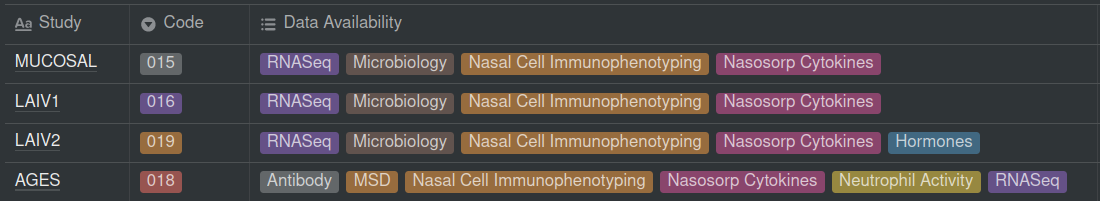
\includegraphics{images/paste-13C4D4A9.png}

Only data without any preprocessing or transformation were used, for all cohorts and data types, except for data retrieved from public databases when additional information was required~in a given~step of the analysis (e.g., GMT files from~Reactome~database for pathway analysis).

Raw data from RNA-Seq experiments consists of~fastq~files and were preprocessed with a benchmark pipeline: samples were aligned using the STAR (Dobin et al., 2013)⁠ software, transcripts~counts~calculated with~featureCounts~(Liao, Smyth, \& Shi, 2014)⁠ software and, with personalized scripts in bash and R language, samples of a given cohort were merge in a single table, where each row represent a transcript and each column a sample. Both STAR and~featureCounts~steps were supplied with the Hg38 reference (Herrero et al., 2016;~Ruffier~et al.,~2017)⁠⁠ genome and features, represented by~Ensembl~identifiers (EnsemblID, Aken et al., 2016), were parsed so that the~EnsemblID`s~version is omitted. Quality control checks were performed between each step of the preprocessing procedure, with~fastQC~(A. \&~Bittencourt~a,~2010)⁠~on~fastq~files before alignment and~MultiQC~(Ewels, Magnusson, Lundin, \&~Käller, 2016)⁠ for all steps with no samples removed due to low quality. Counts data were normalized either with trimmed means of M-values (TMM, Smid et al., 2018)⁠ or variance stabilizing transformation (vst) (Zwiener, Frisch, \& Binder, 2014)⁠with the DESeq2 (Love, Huber, \& Anders, 2014)⁠ package from Bioconductor (Ihaka \& Gentleman, 1996)⁠⁠, when necessary.

For the remaining data types, raw data were retrieved in standard comma/tab-separated formats (e.g.~CSV), containing tables representing either absolute measurements, proportions or mean levels of biological variables (e.g.~EGF, IL-10 for Luminex or T-Cell Percentage for flow cytometry data) in the columns, for a given volunteer and time-point in the rows. Raw values were shifted by a constant value (all values are added by the absolute minimum value of the dataset) to avoid negative/zero value and then log2 transformed. Depending on the analysis step, each variable could be further scaled by the Z-Score transformation. Variables or features with more than 25\% of missing values were excluded, with the remaining missing data imputed through an unsupervised approach algorithm implemented in the~missForest~(Stekhoven~\& Buhlmann,~2012)⁠~package.

Each dataset was further inspected for data quality, outliers and technical artefacts or batch effects, and overall variable distribution. This was done with usual exploratory data analysis (EDA), such as dimensionality reduction algorithms (e.g.~Principal Component Analysis (PCA) and Independent PCA (IPCA)), clustering techniques (e.g.~Hierarchical Clustering (HC)) and visualization tools provided by R packages.

\hypertarget{biological-pathways}{%
\subsection{Biological Pathways}\label{biological-pathways}}

With the results obtained from the analysis of DE and co-expression analysis of RNA-Seq data, we get new sets of variables that could potentially have some biological meaning, as explained in the previous section. For instance, after the identification of DEGs obtained in a certain comparison, we will possibly have two lists of genes that are up- and down-regulated. The same is true for the co-expression analysis, in which we will get a different list of genes for each co-expression module identified during the analysis. All those lists should then be further explored through enrichment analysis to identify which biological pathways are most probably related in order to uncover the underlying molecular mechanisms.

To identify which biological pathways could potentially be perturbed in each comparison of a DE analysis, gene set enrichment analysis (A. Subramanian et al.,~2005)⁠~was performed upon the ranked log2FC values. The~Reactome~(Croft et al.,~2011)⁠~gene set (GMT file) from~Enrichr~(Chen et al., 2013; Kuleshov et al.,~2016)⁠~database was retrieved from~Enrichr~database. Also, the~EnsemblIDs~of each transcript was translated into Gene Symbol IDs with the~biomaRt~(Durinck, Spellman, Birney, \& Huber,~2009)⁠~package so the transcripts could be matched between the datasets and~Reactome~gene set. The actual enrichment was performed with the~fgsea~function from~fgsea~(Sergushichev,~2016)⁠~package, with all parameters set as default, except for the number of permutations (nperm) that was set to 1000. The enrichment results of each comparison were merged with all comparison in each analysis, and all pathways with~padj~\textless{} 0.05 in at least one of the comparisons were selected to further exploratory analysis. To further explore such selected pathways, common pathways for all groups or time-points were displayed in correlation~plots, from~corrplot~(Wei \& Simko, 2017)⁠ package, with pathways represented in rows, comparison represented in columns and enrichment (NES) values as circles,~coloured~in a blue-to-red gradient, representing negative to positive perturbation respectively.

\hypertarget{proposed-solution}{%
\section{Proposed Solution}\label{proposed-solution}}

\hypertarget{overall-data-analysis}{%
\subsection{Overall Data Analysis}\label{overall-data-analysis}}

\hypertarget{identification-of-perturbed-features}{%
\subsubsection{Identification of Perturbed Features}\label{identification-of-perturbed-features}}

To first answer the most basic question, ``which biological variable(s) are possibly related to~Spn~inoculation?'', features that suffered any perturbation were detected through statistical methods which compare their sample distribution after the inoculation to its baseline levels. In RNA-Seq data, this analysis is performed with both DESeq2 and~edgeR~(Robinson, McCarthy, \& Smyth,~2009)⁠~R packages and it is known as differential expression analysis (DEA). This perturbation is represented by the ratio of distribution means and displayed as log2 fold-change (log2FC) values. Statistical confidence is also estimated, represented by the p-values (pval), and further adjusted (padj) for multiple comparisons. Deferentially expressed genes (DEG) can be selected by setting thresholds for both log2FCs and p-values, and classified in up-, down-regulated or unperturbed according to its log2FCs direction. In this study DEGs were defined according to the following thresholds: among the genes with~padj~\textless{} 0.01 the ones with log2FC \textgreater{} 0 are classified as UP, log2FC \textless{} 0 classified as DOWN and the remaining as UNCHANGED.

Similar statistical tests were applied to the remaining data types using R core functions. These tests can be parametric (e.g.~T-Test) or not (e.g.~Mann-Whitney-Wilcoxon (MWW test) and are applied accordingly if most of the variables~in a given~dataset follow a normal distribution or not, respectively. P-values obtained from these tests were corrected for multiple comparisons with Bonferroni method (Armstrong,~2014)⁠~and variables with~\emph{padj}~below a threshold of 0.01 were selected for further analysis.

\hypertarget{identification-of-transcriptional-programs-and-variables-cluster-with-similar-patterns}{%
\subsubsection{Identification of Transcriptional Programs and Variables Cluster with Similar Patterns}\label{identification-of-transcriptional-programs-and-variables-cluster-with-similar-patterns}}

Beyond identifying perturbed variables, one might want to discover groups of variables that have similar patterns throughout the time-points or between conditions. One example of this type of analysis is co-expression analysis, usually performed with transcriptomic data. Such analysis assumes that genes with similar~behaviour~or pattern of expression could be biological entities that are working together, potentially representing a biological program and perhaps being orchestrated by common regulators. For example, a given set of highly correlated genes could indicate that they are all member of the apoptosis mechanism and might even be regulated by the same transcriptional factor, long non-coding RNA (lincRNAs) or~micro RNA~(miRNA). This type of analysis is very powerful to identify major patterns in the data, being them transcriptomic data or not.

In the case of RNA-Seq data, co-expression analysis were performed using the~CEMiTool~(Russo et al., 2018)⁠ package, which allow the identification of co-expression modules (MOD), visualize their overall expression along samples, identify most probable biological pathways that a given MOD could be related to and also analyze how each module are behaving in each condition or time-point, in other words, identify if the given module is up- or down-regulated in each condition/time-point by analyzing if the majority of its constituents (genes/transcripts) are highly enriched among the highly positively or negatively expressed genes.

The same basic idea was also applied to the other types of data in order to identify possible relationship patterns among the biological variables. For example, identifying sets of cytokines (Luminex) or immune cell types (flow cytometry) that are highly correlated between each other, either across time-points or groups (e.g.~Spn~groups, vaccine type, etc.). This sets of highly correlated variables were determined through the calculation of pairwise correlations (Spearman, Rho) for all variables in each dataset. These pairwise correlations are represented in the form of a correlation matrix, with the number of rows and columns equal to the total number of variables present in the dataset. To define if two variables are connected or not, discrete values of 0s and 1s were used to represent if a connection exists, respectively. Values of 1 were assigned if their absolute correlation values were \textbar Rho\textbar{} \textgreater= 0.7, 0 otherwise. This discrete matrix, also known as an adjacency matrix, was used to create a graph, where the nodes represent biological variables (e.g.~cytokines, cell type) and can be connected (edges) only if its adjacency value is equal to 1. Finally, variables were grouped into modules through the Louvain (Newman, 2006;~Traag, Waltman, \& van Eck,~2019)⁠~clustering method, a commonly used community detection algorithm and available in~igraph~(Csárdi~\&~Nepusz, n.d.)⁠ package.

\hypertarget{transcriptomics-analysis-pipeline}{%
\section{Transcriptomics Analysis Pipeline}\label{transcriptomics-analysis-pipeline}}

\hypertarget{quality-control}{%
\subsection{Quality Control}\label{quality-control}}

\begin{itemize}
\item
  Density plot
\item
  Clustering
\item
  MA plot

  \begin{itemize}
  \item
    microarray - affycoretools::maplot() - \url{https://rdrr.io/bioc/t/man/maplot.html}
  \item
    rnaseq - DESeq2::plotMA(dds)
  \end{itemize}
\item
  Distribution (Normality) test
\item
  PVCA
\item
  MDP
\item
  RLE
\item
  Multidimensional scaling (MDS)
\item
  Bi-clustering
\item
  PCA
\item
  IPVCA
\item
  mixOmics
\end{itemize}

\hypertarget{biomarkers}{%
\subsection{Biomarkers}\label{biomarkers}}

\begin{itemize}
\item
  DEG Analysis

  \begin{itemize}
  \item
    Microarray

    \begin{itemize}
    \tightlist
    \item
      distribution assumptions evaluation
    \end{itemize}
  \end{itemize}
\item
  RNA-Seq

  \begin{itemize}
  \item
    DESeq2
  \item
    edgeR
  \item
    limma
  \end{itemize}
\item
  DE analysis:

  \begin{itemize}
  \item
    limma
  \item
    t-test
  \item
    ANOVA
  \item
    ranking methods

    \begin{itemize}
    \tightlist
    \item
      see other methods and approaches
    \end{itemize}
  \item
    \emph{p-value} distribution analysis
  \item
    pathway stabilization for DEGs thresholding
  \end{itemize}
\item
  Bi-clustering

  \begin{itemize}
  \tightlist
  \item
    \url{https://rpubs.com/crazyhottommy/PCA_MDS}
  \end{itemize}
\end{itemize}

\hypertarget{pathway-analysis}{%
\subsection{Pathway Analysis}\label{pathway-analysis}}

\begin{itemize}
\item
  ORA

  \begin{itemize}
  \item
    Network Analyst
  \item
    Enrichr
  \item
    StringR
  \end{itemize}
\item
  GSEA
\item
  IPA
\end{itemize}

\hypertarget{pipeline}{%
\subsection{Pipeline}\label{pipeline}}

INPUT: - Raw expression data - RNA-Seq: counts - Microarray: .CEL, raw expression table (Illumina) - phenodata

\begin{verbatim}
Parameters:
    - split_proportion = c(#train, #test, #validation)
    - response_var = ""
    - preliminary_filter = c(T,F)
\end{verbatim}

OUTPUT: - biomarkers list - my performance assessment - plots

ALGORITHM - Read data - test tables equivalence - split data in train, test and validation sets - (Optional) preliminary filter (e.g, low variance, low mean) - Biomarker detecion - Biomarkers: biomarker list extraction - Biomarkers performance test in train/test dataset - Biomarkers performance test in validation dataset - plots

\hypertarget{section-1}{%
\subsection{}\label{section-1}}

\hypertarget{network-analysis}{%
\section{Network Analysis}\label{network-analysis}}

\hypertarget{co-expression-analysis}{%
\subsection{Co-expression Analysis}\label{co-expression-analysis}}

\begin{itemize}
\tightlist
\item
  WGCNA / CEMiTool
\end{itemize}

\begin{itemize}
\item
  ARACNE
\item
  Topological analysis
\end{itemize}

\hypertarget{data-driven-analysis-of-susceptibility-to-pneumococcal-carriage}{%
\chapter{Data Driven Analysis of Susceptibility to Pneumococcal Carriage}\label{data-driven-analysis-of-susceptibility-to-pneumococcal-carriage}}

In order to understand the development of Spn carriage it is necessary to know if carriage is some kind of random process. in other words, it is necessary to know if a given subject has the same chance of developing carriage as getting heads in a coin flip after being inoculated by Spn. So, the first question is to know if the probability of developing carriage is different than 0.5.

\hypertarget{q1-is-developing-carriage-random}{%
\section{Q1: Is developing carriage random?}\label{q1-is-developing-carriage-random}}

If carriage development is indeed a random process, a given subject would have a probability of 0.5 of becoming carriage positive (POS), as there are only two possible mutually exclusive outcomes: positive (POS) or negative (NEG).

The null hypothesis is that the probability of developing carriage is equal to not developing carriage, P(POS) = P(NEG). The alternative hypothesis is that the probability of developing carriage is different than the probability of not developing carriage, P(POS) \textgreater{} P(NEG) or P(POS) \textless{} P(NEG).

To test these hypothesis, we can estimate such probabilities based on the frequency of volunteers that became carriage POS in the whole EHPC consortium. EHPC provides the density of Spn present in the nasal mucosa after its innoculation from a total of 809 subjects that took part in several studies, as showed in the following graph (Fig 2.1).

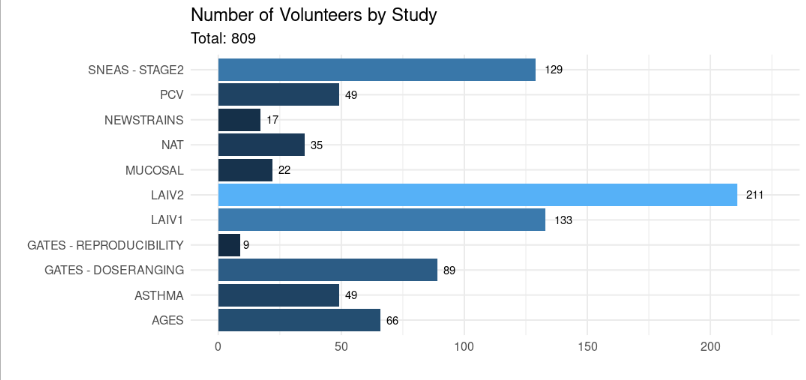
\includegraphics[width=11.19in]{images/paste-1E7F5309}

Based on this data, we arrive at an overall probability equal to 0.447 of developing carriage and a probability \textless{} 0.5 in the majority of the studies, as depicted in the following figures.

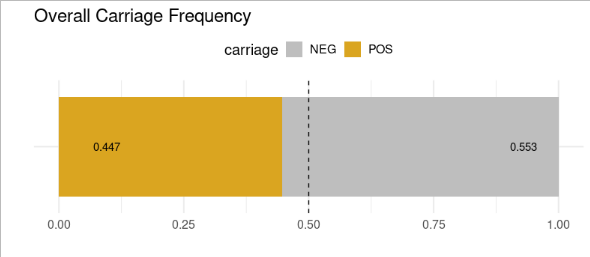
\includegraphics[width=8.19in]{images/paste-10E686C0}

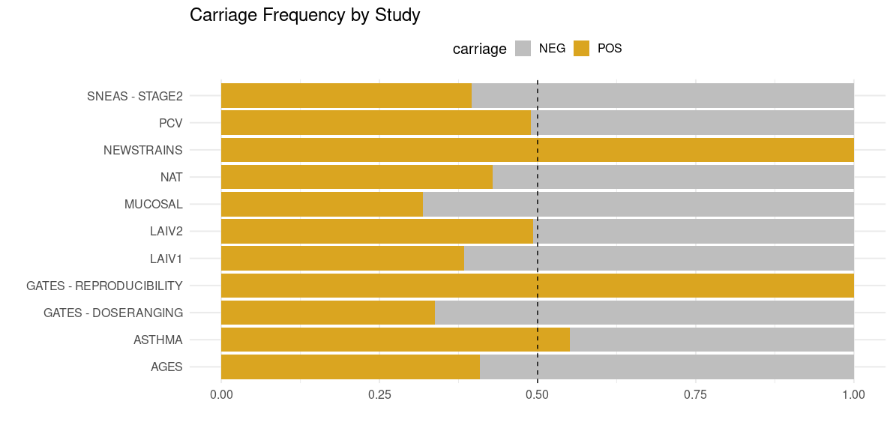
\includegraphics[width=12.4in]{images/paste-CA5BC0AE}

Across all studies women have a higher probability of developing carriage than men (Fig. 2.4), where men have a clear lower (log) odds ratio than women (Fig. 2.5).

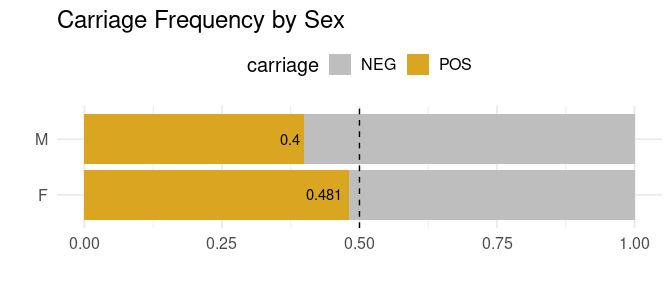
\includegraphics[width=9.33in]{images/paste-3446DB5C}

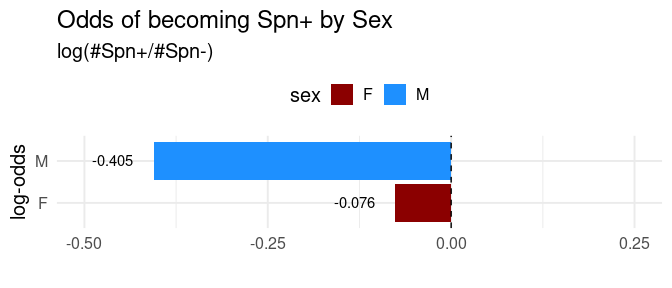
\includegraphics[width=9.33in]{images/paste-1F19DB12}

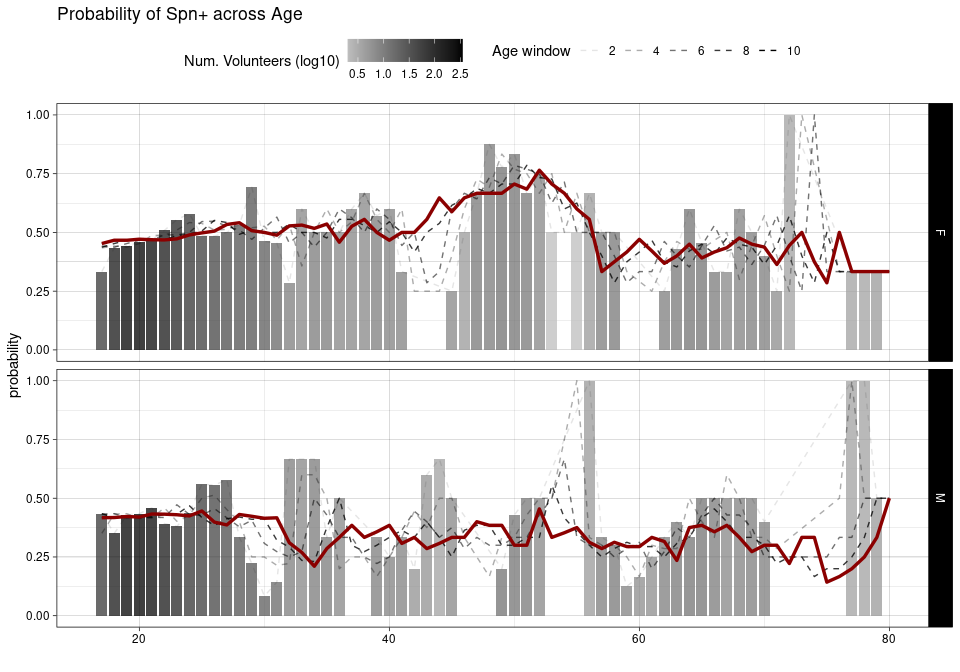
\includegraphics[width=13.33in]{images/paste-986B85C7}

\hypertarget{definitions}{%
\chapter{Definitions}\label{definitions}}

\begin{description}
\item[cross-over design]
is a repeated measurements design such that each experimental unit (patient) receives different treatments during the different time periods, i.e., the patients cross over from one treatment to another during the course of the trial
\item[w. r. t]
with respect to, with regard to
\item[Dependent/outcome variable]
A variable whose value depends upon independent variable, is what is being measured in an experiment or evaluated in a mathematical equation. In the equation a = b/c, the dependent variable, a, is determined by the values of b and c.
\item[Response variables]
The response variable is the variable you are measuring and trying to explain. When you have a response variable, it is always paired with one or more explanatory variables. The explanatory variable(s) drives change in the response variable.
\item[Latent variables]
As opposed to observable variables, are variables that are not directly observed but are rather inferred (through a mathematical model) from other variables that are observed (directly measured).
\item[Covariance]
is a measure of the joint variability of two random variables. Covariance provides a measure of the strength of the correlation between two or more sets of random variates.

\(Cov(x,y) = \Sigma_{i=1,…,N} (x_i - \mu_x)(y_i - \mu_y)/N\)
\item[Linear combination]
A linear combination is an expression constructed from a set of terms by multiplying each term by a constant and adding the results (e.g.~a linear combination of x and y would be any expression of the form ax + by, where a and b are constants).
\item[Independent Component Analysis (ICA)]
Is a statistical and computational technique for revealing hidden factors that underlie sets of random variables, measurements, or signals. In the model, the data variables are assumed to be linear or nonlinear mixtures of some unknown latent variables, and the mixing system is also unknown. The latent variables are assumed non-gaussian and mutually independent, and they are called the independent components of the observed data. These independent components, also called sources or factors, can be found by ICA.
\item[bipartite graphs]
also called a bigraph, is a set of graph vertices decomposed into two disjoint sets such that no two graph vertices within the same set are adjacent.
\item[Discriminant Analysis]
i.g., the prediction of group membership from the levels of continuous predictor variables
\item[Partial Least Squares (PLS) regression]
Partial least squares (PLS) regression is a technique that reduces the predictors to a smaller set of uncorrelated components and performs least squares regression on these components, instead of on the original data. PLS regression is especially useful when your predictors are highly collinear, or when you have more predictors than observations and ordinary least-squares regression either produces coefficients with high standard errors or fails completely. PLS does not assume that the predictors are fixed, unlike multiple regression. This means that the predictors can be measured with error, making PLS more robust to measurement uncertainty.
\item[Multicollinearity (collinearity)]
is a phenomenon in which one predictor variable in a multiple regression model can be linearly predicted from the others with a substantial degree of accuracy. In this situation the coefficient estimates of the multiple regression may change erratically in response to small changes in the model or the data. Multicollinearity does not reduce the predictive power or reliability of the model as a whole, at least within the sample data set; it only affects calculations regarding individual predictors. That is, a multivariate regression model with collinear predictors can indicate how well the entire bundle of predictors predicts the outcome variable, but it may not give valid results about any individual predictor, or about which predictors are redundant with respect to others.

Multicollinearity occurs when your model includes multiple factors that are correlated not just to your response variable, but also to each other. In other words, it results when you have factors that are a bit redundant.

Multicollinearity increases the standard errors of the coefficients. Increased standard errors in turn means that coefficients for some independent variables may be found not to be significantly different from 0. In other words, by overinflating the standard errors, multicollinearity makes some variables statistically insignificant when they should be significant. Without multicollinearity (and thus, with lower standard errors), those coefficients might be significant.

Severe multicollinearity is a major problem, because it increases the variance of the regression coefficients, making them unstable. The more variance they have, the more difficult it is to interpret the coefficients.

Warning Signs of Multicollinearity :

\begin{itemize}
\item
  A regression coefficient is not significant even though, theoretically, that variable should be highly correlated with Y.
\item
  When you add or delete an X variable, the regression coefficients change dramatically.
\item
  You see a negative regression coefficient when your response should increase along with X.
\item
  You see a positive regression coefficient when the response should decrease as X increases.
\item
  Your X variables have high pairwise correlations.
\end{itemize}

Ways to measure multicollinearity: Variance Inflation Factor (VIF): assesses how much the variance of an estimated regression coefficient increases if your predictors are correlated:

\begin{itemize}
\item
  VIF is equal to 1, there is no multicollinearity among factors
\item
  VIF is greater than 1, the predictors may be moderately correlated
\item
  VIF between 5 and 10, indicates high correlation that may be problematic
\item
  VIF above 10, you can assume that the regression coefficients are poorly estimated due to multicollinearity.
\end{itemize}

Dealing with Multicolinearity (VIF near or above 5):

Remove highly correlated predictors from the model. If you have two or more factors with a high VIF, remove one from the model. Because they supply redundant information, removing one of the correlated factors usually doesn't drastically reduce the R-squared. Consider using stepwise regression, best subsets regression, or specialized knowledge of the data set to remove these variables. Select the model that has the highest R-squared value.

Use Partial Least Squares Regression (PLS) or Principal Components Analysis, regression methods that cut the number of predictors to a smaller set of uncorrelated components.
\item[Multivariate/Multivariable Analysis]
(linear) observation and analysis of more than one statistical outcome variable at a time.

Multivariate is used for the analysis with multiple outcomes/dependent variables, whereas multivariable is used for the analysis with multiple explanatory/independent variables. However, they are sometimes used interchangeably in the literature as not many researchers are aware of the difference.

A simple linear regression model has a continuous outcome and one predictor, whereas a multiple or multivariable linear regression model has a continuous outcome and multiple predictors (continuous or categorical). A simple linear regression model would have the form y = a + xb + e. By contrast, a multivariable or multiple linear regression model would take the form y = a + x1b1 + x2b2 + \ldots{} + xkbk + e, where y is a continuous dependent variable, x is a single predictor in the simple regression model, and x1, x2, \ldots, xk are the predictors in the multivariable model.

Multivariate, by contrast, refers to the modeling of data that are often derived from longitudinal studies, wherein an outcome is measured for the same individual at multiple time points (repeated measures), or the modeling of nested/clustered data, wherein there are multiple individuals in each cluster. A multivariate linear regression model would have the form
\item[Orthogonal transformation]
An orthogonal transformation is a linear transformation T:V-\textgreater V which preserves a symmetric inner product: preserves lengths of vectors and angles between vectors
\item[Principal Component Analysis]
Linear transformations of independent varibles of high-dimentional data into lower-dimentionality space, seeking the best directions in the data that account for most of the variability

\begin{verbatim}
Uses: Mainly used for dimensionality reduction and feature extraction   in large datasets.

Others: PCA transforms and project high-dimensional data in a low-dimensional space, by lineary combining the original independent variables in new orthogonal and independent variables that can best explain/highlight the variance present in the data.
\end{verbatim}
\item[principal components]
artificial variables that are linear combinations of the original variables
\item[ill-posed problem]
According to Jacques Hadamard, mathematical models of physical phenomena should have the properties that:

\begin{enumerate}
\def\labelenumi{\arabic{enumi}.}
\tightlist
\item
  a solution exists
\item
  the solution is unique
\item
  the solution's behavior changes continuously with the initial conditions
\end{enumerate}

If the problem is well-posed, then it stands a good chance of solution on a computer using a stable algorithm. If it is not well-posed, it needs to be re-formulated for numerical treatment. Typically this involves including additional assumptions, such as smoothness of solution. This process is known as regularization.

Even if a problem is well-posed, it may still be ill-conditioned, meaning that a small error in the initial data can result in much larger errors in the answers. Problems in nonlinear complex systems (so called chaotic systems) provide well-known examples of instability. An ill-conditioned problem is indicated by a large condition number.
\item[regularization]
is the process of adding information in order to solve an ill-posed problem or to prevent overfitting
\item[overfitting]
is the production of an analysis that corresponds too closely or exactly to a particular set of data, and may therefore fail to fit additiona data or predict future observations reliably. An overfitted model is a statistical lmodel that contains more paramenters than can be justified by the data. The essence of overfitting is to have unknowingly extracted some of the residual variation (i.e., the noise) as if that variation represented underlying model structure.
\item[underfitting]
occurs when a statistical model cannot adequately capture the underlying structure of the data. An underfitted model is a model where some parameters or terms that would appear in a correctly specified model are missing. Underfitting would occur, e.g., when fitting a linear model to non-linear data, tending to have poor predictive performance.
\item[LASSO]
\emph{Least Absolute Shrinkage and Selection Operator.} Regression analysis method that performs both variable selection and regularization in o\textbackslash`\textbackslash`rder to enhance the prediction accuracy and interpretability of the statistical model it produces. Lasso was introduced in order to improve the prediction accuracy and interpretability of regression models by altering the model fitting process to select only a subset of the provided covariates for use in the final model rather than using all of them

Is a regression method that involves penalizing the absolute size of the regression coefficients. By penalizing (or equivalently constraining the sum of the absolute values of the estimates) you end up in a situation where some of the parameter estimates may be exactly zero. The larger the penalty applied, the further estimates are shrunk towards zero. This is convenient when we want some automatic feature/variable selection, or when dealing with highly correlated predictors, where standard regression will usually have regression coefficients that are `too large'.

Generalizations of lasso:

\begin{itemize}
\item
  Elastic net
\item
  Group lasso
\item
  Fused lasso
\item
  Quasi-norms and bridge regression
\item
  Adaptive lasso
\end{itemize}
\item[Factor Analysis]
\href{https://www.theanalysisfactor.com/factor-analysis-1-introduction/}{Factor Analysis} is a statistical method used to describe variability among observed, correlated variables in terms of a potentially lower number of unobserved variables called factors. Is a useful tool for investigating variable relationships for complex concepts such as socioeconomic status, dietary patterns, or psychological scales. Allows researchers to investigate concepts that are not easily measured directly by collapsing a large number of variables into a few interpretable underlying factors.

The key concept of factor analysis is that multiple observed variables have similar patterns of responses because they are all associated with a latent (i.e.~not directly measured) variable. In every factor analysis, there are the same number of factors as there are variables. Each factor captures a certain amount of the overall variance in the observed variables, and the factors are always listed in order of how much variation they explain.

The eigenvalue is a measure of how much of the variance of the observed variables a factor explains. Any factor with an eigenvalue ≥1 explains more variance than a single observed variable. The relationship of each variable to the underlying factor is expressed by the so-called factor loading. Since factor loadings can be interpreted like standardized regression coefficients, one could also say that the variable income has a correlation of 0.65 with Factor 1. This would be considered a strong association for a factor analysis in most research fields.
\end{description}

\hypertarget{appendix-appendix}{%
\appendix}


\hypertarget{essential-literature}{%
\chapter{Essential Literature}\label{essential-literature}}

\hypertarget{thesis}{%
\section{Thesis}\label{thesis}}

\begin{itemize}
\item
  Adler's PhD Thesis → Pneumococcal nasopharyngeal colonisation in adults
\item
  Elena's PhD Thesis → The human lung immune responses to nasopharyngeal pneumococcal colonisation in healthy adults
\item
  Fernando's Master Thesis
\end{itemize}

\hypertarget{articles}{%
\section{Articles}\label{articles}}

\hypertarget{pneumococcal-diseases}{%
\subsection{Pneumococcal Diseases}\label{pneumococcal-diseases}}

\begin{itemize}
\item
  \href{https://journals.plos.org/plospathogens/article?id=10.1371/journal.ppat.1006665}{The immunological mechanisms that control pneumococcal carriage}
\item
  \href{https://pubmed.ncbi.nlm.nih.gov/29599457/}{\emph{Streptococcus pneumoniae}: transmission, colonization and invasion}
\item
  \href{https://pubmed.ncbi.nlm.nih.gov/23818515/}{The Pneumococcus: Epidemiology, Microbiology, and Pathogenesis}
\item
  \href{https://pubmed.ncbi.nlm.nih.gov/30374129/}{Inflammation induced by influenza virus impairs human innate immune control of pneumococcus}
\item
  \href{https://www.researchgate.net/publication/348794084_Pneumococcal_colonization_impairs_mucosal_immune_responses_to_Live_Attenuated_Influenza_Vaccine_in_adults}{Pneumococcal colonization impairs mucosal immune responses to Live Attenuated Influenza Vaccine in adults}
\item
  \href{}{Experimental human pneumococcal carriage models for vaccine research}
\item
  \href{}{Innate and adaptive nasal mucosal immune responses following experimental human pneumococcal colonization}
\end{itemize}

\hypertarget{sex-differences}{%
\subsection{Sex Differences}\label{sex-differences}}

\begin{itemize}
\tightlist
\item
  \href{https://www.sciencedirect.com/science/article/pii/S2211124719313191}{Sex Differences in the Blood Transcriptome Identify Robust Changes in Immune Cell Proportions with Aging and Influenza Infection}
\end{itemize}

\hypertarget{ageing}{%
\subsection{Ageing}\label{ageing}}

\begin{itemize}
\tightlist
\item
  \href{https://www.cell.com/fulltext/S0092-8674(13)00645-4}{The Hallmarks of Aging}
\end{itemize}

\hypertarget{systems-biology}{%
\subsection{Systems Biology}\label{systems-biology}}

\hypertarget{bioinformatics-and-methodologies}{%
\subsection{Bioinformatics and Methodologies}\label{bioinformatics-and-methodologies}}

\begin{itemize}
\tightlist
\item
  \href{https://www.nature.com/articles/nature25753}{Meta-analysis and the science of research synthesis}
\end{itemize}

\begin{itemize}
\tightlist
\item
  \href{https://pubmed.ncbi.nlm.nih.gov/31201239/}{SIMON, an Automated Machine Learning System, Reveals Immune Signatures of Influenza Vaccine Responses}
\end{itemize}

\hypertarget{pneumococcal-diseases-and-immunity}{%
\chapter{Pneumococcal Diseases and Immunity}\label{pneumococcal-diseases-and-immunity}}

\hypertarget{controlled-human-infection-and-rechallenge-with-streptococcus-pneumoniae-reveals-the-protecticve-efficacy-of-carriage-in-healty-adults}{%
\section{Controlled Human Infection and Rechallenge with Streptococcus pneumoniae Reveals the Protecticve Efficacy of Carriage in Healty Adults}\label{controlled-human-infection-and-rechallenge-with-streptococcus-pneumoniae-reveals-the-protecticve-efficacy-of-carriage-in-healty-adults}}

- High rates of disease and death in the elderly are associated with low carriage prevalence.

- Objective: apply an experimental human pneumococcal carriage model ot investigate the immunizing effect of a single carriage episode;

- Carriage increased both mucosal and serum IgG levels to pneumococcal proteins and polysccharide, resulting in a fourfold increase in opsonophagocytic activity;

- passive transfer of postcarriage sera from colonized by a heterologous strain in a murine model of invasive pneumococcal pneumonia. These levels were significanlty higher than the protection conferred by either precarriage sera (30\%) or saline (10\%);

- Responses elicited by a sigle experimentally induced subsequent carriage and mice against invasive pneumococcal disease by passive transfer of sera from clonized individuals.

- We have found no relation of baseline serum IgG and carriage outcome after challenge.

- Intranasal exposure to bacteria boosted serum IgG levels to several pneumococcal prteins, with carriage-positive subjects showing the greatest magnitude of response.

- Persistent increased IgG to proteins was observed in carriage-positive subjects at 5 weeks after inoculation and not in those without carriage.

- The boosting effect of exposure is temporary and therefore different than responses induced by persistent carriage. This increased and sustained carriage acquisition after rechallenge up to 11 months after clearance of the first carriage episode.

\hypertarget{inflammation-induced-by-influenza-virus-impairs-innate-control-of-human-pneumococcal-carriage}{%
\section{Inflammation induced by influenza virus impairs innate control of human pneumococcal carriage}\label{inflammation-induced-by-influenza-virus-impairs-innate-control-of-human-pneumococcal-carriage}}

2know:

\begin{verbatim}
- secondary vs primary bacterial penumonia

- upper respiratory tract

- human type 6B pneumococcal challenge model

- degranulation of neutrophils

- role of neutrophils

- role of monocytes

- within-household Spn transmission

- Live Attenuated Influenza Vaccine

- murine models

-   Th17-dependent recruitment of neutrophils

- Type I interferons

- scavenger receptor MARCO

- double-blinded controlled randomized clinical trial

- tretavalent inactivated influenza vaccine

- nasal lining fluid

- rhinovirus

- coronavirus

- respiratory syncytial virus

- parainfluenzavirus

- luminal neutrophils

- myeloperoxidase (marker for neutrophil degranulation)

- Nanostring expression analysis

- 80,000 CFU per nostril

- lytA qPCR

- systematic LAIV dispensing error

- Neutrophil opsonophagocytic killing
\end{verbatim}

Primary endpoint:

\begin{verbatim}
- the occurence of pneumococcal colonisation determined by the presence of pneumococcus in nasal wash samples (NW) at any time point post inoculation up to and including day 29.
\end{verbatim}

Secondary endpoint:

\begin{verbatim}
- density of pneumococcal colonisation in NW at each time point following pneumococcal inoculation (days 2, 7, 9, 14, 22 and 29)

- the are under the curve of pneumococcal colonisation density following pneumococcal inoculation

- immunological mechanisms associated with altered susceptibility to pneumococcus following LAIV.
\end{verbatim}

- Flow cytometry analysis:

\begin{verbatim}
- nasal cells

- whole blood
\end{verbatim}

- Neutrophil opsonoohagocytic killing

- Luminex analysis of nasal lining fluid or stimulated nasal cells

- RNA extraction and sequencing

\begin{verbatim}
- Illumina Hiseq4000, 20M reads, 100 paired-end reads
\end{verbatim}

- Nanostring

\begin{verbatim}
- Purified blood neutrophils
\end{verbatim}

\hypertarget{sex-differences-1}{%
\chapter{Sex Differences}\label{sex-differences-1}}

\hypertarget{ageing-1}{%
\chapter{Ageing}\label{ageing-1}}

\hypertarget{the-hallmarks-of-aging}{%
\section{The Hallmarks of Aging}\label{the-hallmarks-of-aging}}

We have two different ages:

\begin{verbatim}
- chronological age

    number of years since you were born

- biological age

    the time-dependent decline of your body's function and appearance
\end{verbatim}

Chronological and biological age correlate with each other, so the signs of aging appear around a similar chronological age in most people.

But often people exhibit signs of biological aging at very different rates.

Extreme examples can be found in progeroid conditions-congenital disorders that cause the signs of biological aging to begin at a very young age.

In recent years, scientists studying the molecular and cellular processes that govern these changes and their variation in individuals have identified nine interconnected ``hallmarks of aging''. Determined mainly by our genetics, but modulated by environmental factors, each of these nine hallmarks contributes to the damage that occurs with age and ultimately drives age-associated pathologies.

1. Genomic Instability

2. Telomere attrition

3. Epigenetic alterations

4. Loss of proteostasis

5. Deregulated nutrient sensing

6. Mitochondrial disfunction

7. Cellular senescence

8. Stem cell exhaustion

9. Altered intercellular communication

\hypertarget{therapies}{%
\section{Therapies}\label{therapies}}

- CR mimetics

\begin{verbatim}
may improve nutrient sensing.
\end{verbatim}

- senolytics

\begin{verbatim}
a class of drug that removes senescent cells.

- quercetin (The Achilles'heel of senescent cells: from transcriptome to senolytic drugs)

    senolytic treatment using quercetin signifincantly improved vasomotor function in their mouse test group which due to an increase in nitric oxide bioavailability. They also found that clearing senescent cells reduced aortic calcification and osteogenic signalling in both aged and hypercholesterolemic mice. They noted tjat there was no significant effect on intimal plaque fibrosis by treatment.



It has been demonstrated that senescent cells can be cleared selectively by targeting anti-apoptotic proteins Bcl-2 and Ccl-x, using a number of different inhibitors, leading to improved tissue function in mice:

    Zhu, Yi et al. - The Achiles' Heel of Senescet Cells: From Transcriptome to Senolytic Drugs

    Chang, Jianhui et al. - Clearance of Senescent Cells by ABT263 Reuvenates Aged Hematopoietic Stem Cells in Mice

    Discovery of Piperlongumine as a Potential Novel Lead for the Development of Senolytic Agents

    Identification of a Novel Senolytic Agent, Navitoclax, Targeting the Bcl-2 Family of Anti-apoptotic Factors.

Baar et al. (Targeted Apoptosis of Senescent Cells Restores Tissue Homeostasis in Response to Chemotoxicity and Aging)

The molecule in the Baar et al. study instead functions by disrupting the interaction between Foxo4 and p53, leading to p53 mediated apoptosis (cell death). The authors have shown that this interaction with Foxo4 inactivates p53 and is restricted specifically to senescent cells. This leads to cell cycle arrest and an inhibition of apoptosis. The molecule itself consists of a small peptide of Foxo4, consisting of D-amino acids, in a retro-reversed sequence, fused to and HIV-Tat domain. The D-amino acids block proteolysis of the compound while the HIV-Tat domain functions as a cell penetrating peptide, enabling the molecule to transverse plasma membranes.
\end{verbatim}

\hypertarget{senescent-cells}{%
\section{Senescent Cells}\label{senescent-cells}}

Senescent cells are no longer capable of cell division and they do not support the tissue they are part of. Instead they secreate a cocktail of harmful pro-inflammatory chemical signals that inhibit tissue repair and drive chronic inflammation.

Normally senescent cells are removed and recycled by the immune system but as we age this too begins to decline and more and more senescent cells escape this housekeeping process. It is at that point that cellular senescence ceases being beneficial and protectig us and becomes a driver of the aging process.

Good citizens but bad neihbors - Non-dividing cells would not be a problem themselves but unfortunatelly the secreted pro-inflammatory chemicals they express also encorage nearby healthy cells to enter the same senescent state.

\begin{verbatim}
Collectively this cocktail is known as the Senescent-Associated Secretory Phenotype (SASP)

SASP:

    (The senescece-associated secretory phenotype: the dark side of tumor suppression)

    - inhibits a number of important cellular processes

    - prevents effective tissue repair

    - contributes to chronic background inflammation

    - is implicated in the onset of age-related diseases (Inflammtory networks during cellular senescence: causes and consequences)
\end{verbatim}

Senescent cells contribute to a second hallmark of aging: altered intercellular communication. This is the age-associated low-grade chronica inflammation many researchers call ``inflammaging'' and is another hallmark of the aging process.

Inflammaging

\begin{verbatim}
is caused by:

    - infectious burden

    - cell debris

    - excessive activation of the NF-kB protein complex (regulator of the immune response)

    - senescent cell SASP

interferes with intracellular signalling

contributes to the loss of regenerative capacity in stem cells and tissues
\end{verbatim}

Senescent cells normally destroy themselves via a programmed process called Apoptosis and they are also removed by the immune systme, however the immune system weakens with age and increasing numbers of these senescent cells escape this process and build up. By the time people reach old age significant numbers of these senescet cells have accumulated in the body and inflammation and damage to surrounding cells and tissue.

\hypertarget{the-role-of-senescent-cells-in-aging}{%
\section{The Role of Senescent Cells in Aging}\label{the-role-of-senescent-cells-in-aging}}

- profound chromatin and secretome changes

- tumor-suppressor activation

replicative senescence -\textgreater{} Hayflick - this particular type of senescence is linked to telomere attrition, a process that leads to chromosomal instability and promotes tumorigenesis, supporting the original hypothesis that senescence guards against unrestricted growth of damaged cells.

the physiological relevance of cellular senescence extends beyond tumour suppression into biological processes such as:

\begin{verbatim}
- embryonic development

    10--12

- wound healing 13

- tissue repair 14

- organismal ageing 15,16
\end{verbatim}

Causes and effector pathways of senescence

\begin{verbatim}
Stresses that can induce senescence:

    - telomere erosion

    - DNA lesions

    - ROS

        What they all have in common is that they activate the DNA damage response (DDR), a signaling pathway in which ATM or ATR kinases block cell-cycle progression through stabilization of p53 and transcriptional activation of the cyclin-dependent kinase (Cdk) inhibitor p21.

    - Activated oncogenes

        Oncogenic Ras acts through overexpression of Cdc6 and suppression of nucleotide metabolism, causing aberrant DNA replication, formation of double stranded DNA breaks(DSBs) and activation of the DDR pathway (20,21)

    - senescence caused by E2F3 activation or c-Myc inhibition is DDR-independent and involves p19-Arf and p16-Ink4a (17,22).

    - BRAF (V600E) is also DDR-independent and induces senescence through a metabolic mechanism involving up regulation of mitochondrial pyruvate dehydrogenase(23).

    - various tumour suppressors trigger a senescent growth arrest when inactivated, including RB, PTEN, NF1 and VHL (17,26).

        Of these, RB inactivation engages the DDR (26), whereas the others are DDR-independent and act through p19Arf and p16Ink4a.

    - Prolonged exposure to interferon-b also induces senescence, demonstrating that chronic mitogenic signalling outside the context of neoplastic transformation can stimulate senescence (28).

    - epigenetic, nucleolar and mitotic spindle stresses.

        genome-wide chromatin decompression by exposure to histone deacetylase inhibitors triggers senescence via a p21 dependent mechanism (29).

        A key target of epigenetic stressors that promote senescence may be the INK4a/ARF locus, which in proliferating cells is repressed by polycomb group-mediated H3K27 methylation and H2A-K119 ubiquitination (30). Nucleolar stress caused by RNA polymerase I inhibitors triggers a robust p53-mediated senescence response (31).

    - Senescence can also be elicited by suboptimal expression of proteins implicated in spindle formation or mitotic checkpoint control, including human TACC3 and murine BubR1, Bub3 an dRae1, all of which engage p53 and p21 independently of the DDR, often in combination with p16-Ink4a (15,32,33).
\end{verbatim}

A notable species-specific difference is that senescence pathways of murine cells are more dependent on p19Arf than senescence in human cells (27).

Senescence is a multi-step evolving process

Acute vs chronic senescence

Senescence of post-mitotic cells

Senescence in aging and age-related disease

Senescent-cell clearance and future directions

\hypertarget{bioinformatics}{%
\chapter{Bioinformatics}\label{bioinformatics}}

\hypertarget{bioinformatics-essentials}{%
\section{Bioinformatics Essentials:}\label{bioinformatics-essentials}}

\begin{verbatim}
- Programming
    - R basics
        variables
        basic operations
        logic operations
        functions
        data reading and writing
        data frame manipulations
        merging
        Workflow and Projects
        Programming Skills
        - Pipes
        - Functions
        - Vectors
        - Iteration (loops)
        - Graphs
        3. Important (frequent) Types of Data
        - Relational data
            https://r4ds.had.co.nz/relational-data.html
            will give you tools for working with multiple interrelated datasets.

        - Strings:
            https://r4ds.had.co.nz/strings.html
            will introduce regular expressions, a powerful tool for manipulating strings.

        - Factors
            https://r4ds.had.co.nz/vectors.html#factors-1
            are how R stores categorical data. They are used when a variable has a fixed set of possible values, or when you want to use a non-alphabetical ordering of a string.

        - Dates and times
            https://r4ds.had.co.nz/dates-and-times.html#dates-and-times
            will give you the key tools for working with dates and date-times.

    - Bash
    - Python

- Statistics:
    - distributions
    - T test
    - ANOVA
    - correlation
    - regression
    - PCA
    - Multivariate Analysis
    - Bayesian statistics

- Linear Algebra (very basics, mostly to understand PCA)
    
- Exploratory Data Analysis (EDA)
    Olhar:
    https://rpubs.com/crazyhottommy/PCA_MDS
    http://girke.bioinformatics.ucr.edu/GEN242/mydoc_Rclustering_3.html
    https://rstudio-pubs-static.s3.amazonaws.com/93706_e3f683a8d77244a5b993b20ad6278f4b.html

    1. Data Wrangling
        - Data Import (https://r4ds.had.co.nz/data-import.html)         
        - Tidy data (https://r4ds.had.co.nz/tidy-data.html)
    2. Data Understand Cycle
    (Transform -> Visualise -> Model -> Transform -> ...)
        - Variation
        - Outliers
        - Covariation
        - Patterns and Models

    3. Communicate
        Data Visualisation
        Low-Dimensional Data Visualisation
            Continuous-Continuous
            Continuous-Categorical
            Categorical-Categorical
            
        High-Dimensional Data Visualisation
            Principal Component Analysis (PCA)
            Multidimensional Scaling (MDS)

- Bioinformatics Data Retrieval
    - GEO
    - ArrayExpress
    - TGAC

- Microarray preprocessing:
    - Main technologies: Illumina, Affymetrix and Agilent
    - Quality control
        - ArrayQualityMetrics
        - other technologies

    - Normalization
        - RMA
        - quantile

    - Batch analysis:
        - PCA
        - PVCA
        - RLE
    - Missing values:
        - data imputation
        - variable/sample removal assessment

- Basic Analysis
    - Differential Gene Expression Analysis
        - limma

    - Clustering
        - hierarchical clustering
        - k-means
        - density-based clustering

    - Co-expression Analysis
        - WGCNA
        - CEMITOOL

    - Enrichment Analysis
        - ORA
        - GSEA
        - arbitrary search for Consistent Enrichment Gene AnalySis (asCEGAS)
        - more advanced ones


- Machine learning:
    - Regression:
        - linear regression
        - polynomial regression
        - ridge/lasso/elastic net regression
        - SVM
        - Decision Trees
        - Random Forest
        - neural networks

    - Classification:
        - logistic regression
        - SVM
        - Decision Tress
        - Random Forest
        - neural networks
    - Model performance evaluation
    - Variable Importance
    - Feature Selection
        - forward/backward selection

- Dimensionality Reduction
    - Feature Selection/elimination
    - Feature Engineering/extraction

- Data Integration
    - MixOmics

- loose things
    - scree plot
    - Oranges
    - Regression Plots
    - gradient descent
    - heteroskedasticity
    - Independent Component Anaysis
    - Factor Analysis
    - Discriminant Analysis
\end{verbatim}

External Resources:

\begin{verbatim}
Books:
    - Livro Draghici (microarray analysis bible)
\end{verbatim}

\hypertarget{differential-expression-analysis}{%
\section{Differential Expression Analysis}\label{differential-expression-analysis}}

Differential gene expression analysis

\url{https://www.youtube.com/watch?v=5tGCBW3_0IA}

Normalization

Dispersion estimation

Log fold change estimation

Statistical testing

Filtering

Multiple testing correction

--- NORMALIZATION

for comparing gene expression between (groups of) samples, normalize for

\begin{itemize}
\item
  library size (number of reads obtained)
\item
  RNA composition effect
\end{itemize}

The number of reads for a gene is also affected by transcript length and GC content

\begin{itemize}
\tightlist
\item
  When studyin differential expression you assume that they stay the same
\end{itemize}

``FPKM and TC are ineffective and should be definitely abandoned in the context of differential analysis''

"In the presence of high count genes, only DESeq and TMM (edgeR) are able to maintain a reasonable false positive rate without any loss of power

Do NOT use RPKM/FPKM for differential expression analysis!

\begin{itemize}
\item
  Reads (or fragments) per kilobase per million mapped reads.
\item
  Normalizes for gene length and library size:
\item
  20kb transcript has 400 counts, library size is 20 million reads
\end{itemize}

=\textgreater{} RPKM = (400/20)/20 = 1

\begin{itemize}
\tightlist
\item
  0.5 kb transcript has 10 counts, library size is 20 million reads
\end{itemize}

=\textgreater{} RPKM = (10/0.5)/20 = 1

\begin{itemize}
\item
  RPKM/FPKM can be used only for reporting expresison values, not for testing differential expression
\item
  In DE analysis raw counts are needed to assess the measurement precision correctly
\end{itemize}

--- NORMALIZATION BY edgeR and DESeq

= Aim to make normalized counts for non-differentially expressed genes similar between samples

\begin{itemize}
\tightlist
\item
  do not aim to adjust count distributions between samples
\end{itemize}

= Assume that

\begin{itemize}
\item
  Most genes are not differentially expressed
\item
  Differentially expressed genes are divided equally between up- anbd down-regulation
\end{itemize}

= Do not transform data, but use normalization factors within statistical testing

Normalizatio by edgeR/DESeq2 - how?

= DESeq2

\begin{itemize}
\item
  take geometric mean of tene`s counts across all samples
\item
  divide gene's coutns in a sample by the geometric mean
\item
  take median of these raios -\textgreater{} sample's normalization factor (applied to read counts)
\end{itemize}

= edgeR

\begin{itemize}
\item
  Select as reference the sample whose upper quantile is closest to the mean upper quartile
\item
  log ratio of gene`s counts in sample vs reference -\textgreater{} M value
\item
  take weighted trimmed mean of M-values (TMM) -\textgreater{} normalizatio factor (applied to library sizes)
\item
  trim: exlclude genes with high counts or large differneces in expresion
\item
  weights are from the delta method on binomial data
\end{itemize}

\hypertarget{empirical-assessment-of-analysis-workflows-for-differential-expression-analysis-of-human-samples-using-rna-seq}{%
\subsection{Empirical assessment of analysis workflows for differential expression analysis of human samples using RNA-Seq}\label{empirical-assessment-of-analysis-workflows-for-differential-expression-analysis-of-human-samples-using-rna-seq}}

Unknowns:

- flow cytometry

\begin{verbatim}
In biotechnology, flow cytometry is a laser or impedance-based, biophysical technology employed in cell counting, cell sorting, biomarker detection and protein engineering, by suspending cells in a stream of fluid and passing them by an electronic detection apparatus.

- impedance

    Electrical impedance is the measure of the opposition that a circuit presents to a current when a voltage is applied. In quantitative terms, it is the complex ratio of the voltage to the current in an alternating current (AC) circuit.
\end{verbatim}

- precision \& recall

\begin{verbatim}
precision (also called positive predictive value) is the fraction of retrieved instances that are relevant

proportion of retrieved set that are in fact relevant

P = Pr(relevant \| retrieved) = TP / (TP + FP)

intuition: how much junk did we give to the user?

recall - fraction of all relevant documents that were found

R = Pr(retrieved \| relevant) = TP / (TP + FN)

intuition: how much of the good stuff did we miss?

also known as sensitivity, is the fraction of relevant instances that are retrieved

Recall in this context is also referred to as the true positive rate or sensitivity, and precision is also referred to as positive predictive value (PPV)

Accuracy involves how close you come to the correct result and your accuracy improves with tools that are calibrated correctly

Precision is how consistently you can get that result using the same method
\end{verbatim}

- Expression Modeler

\begin{verbatim}
swiftly - rapidamente

paucity - escassez

thawed - descongelado

analytes - analitos (Analito é uma substância ou componente químico, em uma amostra, que é alvo de análise em um ensaio)
\end{verbatim}

- PPLR

1. Background

\begin{verbatim}
    - estimating expression from short sequence reads poses unique problems such as accurate read alignment in the presence of sequencing errors, measurement bias depending on library preparation methodology, and complexity in estimating the expression of distinct mRNA transcripts with shared exons.

    - the optimal

workflow for a given application remains a subject of

intensive investigation.

    - The three major steps of differential expression analysis by RNA-Seq are:

        + alignment of reads to an annotated genome (or less commonly, ab initio reconstruction of a transcriptome annotation)

        + expression modeling to obtain gene-level and/or transcript-level expression estimates

        + statistical analysis to identify differentially expressed genes or transcripts between comparison groups.

    - the ultimate evaluation of any given tool must take into consideration the samples to which it will be applied and the workflow context in which it will be employed.

    - We find that

different RNA-Seq analysis workflows differ widely in

their performance, as assessed by recall, or the propor-

tion of reference-identified genes that were also identi-

fied by the given workflow, and precision, or the

proportion of genes identified by the workflow that were

also identified by the reference.

    - Many workflows per-

form equally well, but are calibrated differently with re-

spect to favoring higher recall or precision, with an

inverse relationship between these parameters.

    - we recommend that the selection of a

given approach be guided by the tolerance of down-

stream applications for type I and type II errors.
\end{verbatim}

2. Methods

\begin{verbatim}
2.1 Samples

2.2 RNA sequencing

2.3 Read alignment, expression modeling, and differential expression identification

    all code are available at <https://github.com/cckim47/kimlab/tree/master/rnaseq.>

    Reads were aligned to release GRCh37 of the human genome.

    Reads were aligned with:

        - Bowtie2

        - HISAT2

        - Kallisto

        - Salmon

        - Sailfish

        - SeqMap

        - STAR

        - TopHat2

    Gene and transcript expression was estimated with:

        - BitSeq

        - cufflinks

        - htseq

        - IsoEM

        - Kallisto

        - RSEM

        - rSeq

        - Sailfish

        - Salmon

        - STAR

        - Stringtie

        - eXpress

    Expression matrices for differential expression input were generated using custom scripts as well as the prepDE.py script provided at the Stringtie website.

    Differentially expressed genes or transcripts were identified with Ballgown, baySeq, BitSeq, cuffdiff, DESeq2, EBseq, edgeR exact test, limma coupled with vst or voom transformation, NBPseq, NOISeqBIO, SAMseq and Sleuth.

        Of these, all but Ballgown, BitSeq, NBPSeq, SAMSeq, and Sleuth used intrinsic filtering or recommended extrinsic filtering of genes or transcripts prior to testing.

        For Sailfish and Salmon, outputs were converted to a Sleuth-ready format using wasabi [55].

        For Kallisto, Sailfish, Salmon, and BitSeq, transcript-level values were condensed to gene-level values using tximport prior to evaluating gene-level differential expression [56].

    For all differential expression analyses performed at the transcript-level, significant transcripts were converted to the corresponding gene for performance evaluation, such that if a single transcript was called as differentially expressed, the corresponding gene was also called differentially expressed.

    All software was run at a detection level of alpha of 0.05, FDR of 0.05, or PPLR in the most extreme 0.05.

2.4 Preparation of reference datasets

    series matrix files were:

        1. downloaded from the NCBI Gene Expression Omnibus

        2. log 2 transformed if necessary

        3. full-quantile normalized

            Smyth GK. Linear models and empirical bayes methods for assessing differential expression in microarray experiments. Stat Appl Genet Mol Biol. 2004;3:1--25.

        4. analyzed for statistically significant gene expression between classical and nonclassical monocytes.

            To reduce bias introduced by a single statistical method, we employed two approaches:

                - Significance Analysis of Microarrays (SAM) [58] with a false discovery rate of 0.05

                    Tusher VG, Tibshirani R, Chu G. Significance analysis of microarrays applied to the ionizing radiation response. Proc Natl Acad Sci U S A. 2001;98:5116--21.

                - limma [59, 60],with a BH-adjusted p-value of 0.05.

                    Kim CC, Falkow S. Significance analysis of lexical bias in microarray data. BMC Bioinformatics. 2003;4:12.

                    Smyth GK. Limma: linear models for microarray data. In: Gentleman R, Carey VJ, Huber W, Irizarry RA, Dudoit S, editors. Bioinforma. Comput. Biol. Solut. Using R bioconductor [internet]. New York, NY: Springer New York; 2005. p.397--420. Available from: <http://dx.doi.org/10.1007/0-387-29362-0_23.>

            Performance of the workflows against both SAM and limma were compared to one another and found to exhibit good reproducibility regardless of the

            statistical method used to generate the data; as such, we chose to use the genes at the intersection of the two methods for our final reference gene sets.

2.5 Quantification of recall and precision

    Because absolute recall and precision values are influenced by the repertoire of analytes that can be measured by a given platform, they used only the common genes.

    Recall was calculated as the number of significant genes in the intersection of the test RNA-Seq datasetwith the reference dataset, divided by the number of genes

    identified as significant in the reference dataset.

    Precision was calculated as the number of significant genes in the intersection of the test RNA-Seq dataset with the reference dataset, divided by the number of genes identified as significant in the test RNA-Seq dataset.
\end{verbatim}

3. Results and discussion

\begin{verbatim}
3.1 Generation of a real-world RNA-Seq dataset for benchmarking

3.2 Overview of empirical testing

    we found that performance of various RNA-Seq workflows was remarkably consistent across all four reference datasets.

    We note, however, that these reference datasets are also subject to the inherent biases of the experimental and computational methods used to produce them.

3.3 Differential influence of workflow stages

    In general, more significant genes were observed when evaluations were performed at the transcript level, because there are more transcripts than genes to potentially be differentially expressed.

    we observed substantial variability in the number of differentially expressed genes identified (n = 208 to 9,489 significant genes)

    Beyond the overall variation, two trends were apparent when the number of genes identified was examined on a by-tool basis:

        1. the differential expression tool had a larger impact on the number of genes identified than the read aligner and expression modeler

            Consequently, the coefficient of variation of the medians was largest for differential expression tools, as compared to read aligners and expression modelers, when assessed at both the gene level (20.5 versus 9.9 and 9.8, respectively) and the transcript level (43.4 versus 10.8 and 39.3).

        2. differential expression tools varied in their robustness to different inputs, with some tools exhibiting relatively reproducible predictions regardless of   the read aligner and expression modeler choices and expression units (e.g., Ballgown), and other differential expression analysis tools exhibiting a wide    range of predictions as the input parameters varied.

    We also evaluated performance of the workflows by calculating recall (intersecting significant genes divided by total number of significant reference genes) and precision (intersecting significant genes divided by total number of significant genes identified by RNA-Seq), using the microarray datasets as references:

        for both precision and recall, the largest effects were observed in workflows differing in the statistical analysis of differential expression, as indicated by the increased medians of differences for this step

3.4 heterogeneiry in performance characteristics of different workflows

    Recall across the workflows was highly correlated with the number of genes identified (Fig. 5a, b). This was true regardless of which of the reference datasets was used for comparison

    The relative rankings of the workflows, ordered by absolute recall value, tended to be consistent across reference datasets

        For gene-level predictions, a subset of workflows using SAMseq exhibited the highest recall values;

        for transcript-level predictions, workflows using baySeq and NBPSeq exhibited the highest recall.

        However, there were exceptions to these rules, depending on the choice of read aligner and expression modeler.

    Precision was highly inversely correlated with the number of genes predicted across the workflows

    Rankings were generally consistent regardless of which reference dataset was used, as was the overall relationship between significant genes and precision

        For gene-level predictions, a subset of workflows using NOISeqBIO exhibited the highest precision, whereas for transcript-level predictions those with the highest precision used several different combinations of tools, with the most prevalent being Ballgown and NOISeqBIO. Strikingly, when used on transcript-level data, the commonly used combination of TopHat2, cufflinks and cuffdiff exhibited one of the highest precision values, coupled with the second lowest number of differentially expressed genes identified

3.5 Performance tradeoff

    the workflows employing NOISeqBIO that exhibit the highest precision were also among those with the lowest recall

    An investigation of the relationship between precision and recall revealed that this tradeoff generally persisted throughout, with many workflows following an inverse linear relationship between precision and recall.

        This held true for both gene- and transcript-level analysis, was true regardless of the expression estimation units, and was also consistent across reference datasets

    the differential expression step had the greatest impact on the performance of each workflow along the spectrum of recall and precision.

    Specific tools that tended to track along this linear tradeoff were Ballgown, DESeq2, limma + voom, limma + vst and SAMseq;

    baySeq and EBseq consistently deviated the furthest.

    SAMseq, one tool with a nonparametric approach, has been highlighted as a high performer previously, in particular when there are a large number of replicates available to approximate the underlying distribution, as is the case here; it performs well, though it does exhibit a tendency toward higher recall at the expense of precision.

    NOISeqBIO, the other tested differential expression tool that assumes a nonparametric distribution, has previously been observed to identify fewer differentially expressed genes with larger sample sizes; we also observe this, as well as correspondingly low recall values.

    Of the differential expression methods tested, baySeq and EBseq are the most similar to each other in underlying statistical methodology; both use an underlying negative binomial model, and then estimate a posterior probability of being differentially expressed for each gene. The observation that EBseq deviated furthest from the precision/recall performance line, due to decreased precision without gains in recall, is similar to previous observations showing that EBSeq tended to produce many false positives with large sample sizes. When applied to gene-level data, baySeq performed similarly to EBseq though not as extreme, with relatively low recall without commensurate gains in precision, which may reflect the similarity in their underlying methods.

    All three linear model workflows perform well and track along the linear precision/recall tradeoff, irrespective of upstream processing. However, there is some difference in default tuning, as Ballgown results tended towards higher precision, whereas limma + voom and limma + vst tended towards higher recall.

    Using BitSeq as the expression modeler tended to result in identification of large numbers of differentially expressed genes, but only in combination with

    differential expression tools that used an underlying negative binomial model for expression data (BaySeq, DESeq2, edgeR, and NBPSeq);

    EBSeq was the one exception, with the number of differentially expressed genes within range of workflows using differential expression tools that model other distributions (Ballgown, BitSeq, limma, and NOISeqBIO).

    We note that BitSeq was unusual in that its most prevalent estimated expression count value was between 1 and 2, rather than less than 1 as most expression modelers estimated; this likely explains why these expression data were poorly modeled by a negative binomial distribution.

    using STAR as the read aligner, most notably with Ballgown as the differential expression tool, led to some of the highest performance workflows having a balance of precision and recall. Interestingly, these best performing workflows are not combinations of aligner and estimator that are suggested by the Ballgown authors, demonstrating the utility of broad, empirical exploration for uncovering improved workflows.    

    the selection of a specific workflow should be largely influenced by the tolerance of a specific application for type I versus type II errors. However, it is also important to note that a significant number of workflows deviated from the roughly linear relationship between recall and precision, particularly for tools targeted at gene-level analyses; such workflows could be considered to exhibit lower performance, as higher performance workflows would be available as alternatives at a given recall or precision target value.

    our findings reflect a defined set of parameters, such as read length, sequencing coverage, sample number, and genetic polymorphism. Thus, it is possible that the performance, both absolute and relative, of the above workflows could vary under other conditions, as some studies have observed

        Kanitz A, Gypas F, Gruber AJ, Gruber AR, Martin G, Zavolan M. Comparative assessment of methods for the computational inference of transcript isoform abundance from RNA-seq data. Genome Biol. 2015;16:150.

        Soneson C, Delorenzi M. A comparison of methods for differential expression analysis of RNA-seq data. BMC Bioinformatics. 2013;14:91.

    Importantly, when selecting a pipeline it is essential to consider not only the specific tools selected at each stage of the workflow, but also how they interact with one another.
\end{verbatim}

4. Conclusions

\hypertarget{network-analysis-1}{%
\section{Network Analysis}\label{network-analysis-1}}

\hypertarget{genemania-a-real-time-multiple-association-network-integration-algorithm-for-predicting-gene-function}{%
\subsection{2008 - GeneMANIA: a real-time multiple association network integration algorithm for predicting gene function}\label{genemania-a-real-time-multiple-association-network-integration-algorithm-for-predicting-gene-function}}

- A new algorithm that is as accurate as the leading methods while capable of predicting protein function in real-time.

\begin{verbatim}
- use a fast heuristic algorithm, derived from ridge regression, to integrate multiple functional association networks and predict gene function from a single process-specific network using label propagation.

- gene function prediction through extrapolation of the functional properties of known genes.

- Genes with similar patterns of expression, synthetic lethality, or chemical sensitivity often have similar functions.

- function tends to be shared among genes whose gene products interact physically, are part of the same complex, or have similar three-dimensional structures.

- Computational analyses have also revealed shared function among genes with similar phylogenetic profiles or with shared protein domains.

- more accurate predictions can be made by combining multiple heterogeneous sources of genomic and proteomic data.

- guilt-by-association principle.
\end{verbatim}

\hypertarget{the-genemania-prediction-server-biological-network-integration-for-gene-prioritization-and-predicting-gene-function}{%
\subsection{2010 - The GeneMANIA prediction server: biological network integration for gene prioritization and predicting gene function}\label{the-genemania-prediction-server-biological-network-integration-for-gene-prioritization-and-predicting-gene-function}}

Questions

Points

\begin{verbatim}
- input: gene list

- GeneMANIA extends the user's list with genes that are functionally similar, or have shared properties with the initial query genes, and displays an interactive functional association network, illustrating the relationships among the genes and data sets.

- Users interested in prioritizing gnes for planning a functional screen can use GeneMANIA to return ranked lists of genes likely to share phenotypes with those in the query list based on GeneMANIA's large and diverse data collection

- it assigns weights to data sets based on how useful they are for each query.

    -\> Individual datasets are represented as networks, and in the basic algorithm, each network is assigned a weight primarily based on how well connected genes in the query list are to each other compared with their connectivity to non-query genes.

    -\> GeneMANIA's adaptive wwigting methods also detect and down-weight redundant networks. This is useful for determining how genes in a gene list are connected to one another, or for determining which types of functional genomic data are most useful to collect for finding more genes like those in the query list.

- Organisms and identifiers:

    -\> support six organism:

        - yeast (Saccharomyces cerevisiae)

        - worm (Caenorhabditis elegans)

        - fly (Drosophila melanogaster)

        - mouse (Mus musculus)

        - Arabidopsis thaliana

        - human (Homo sapiens)

    -\> 747 data sets:

        - 276 co-expression networks, from GEO;

        - 232 physical interaction, from BioGRID;

        - 24 genetic interaction, from BioGRID;

        - 14 co-localization, from Pathway Commons;

        - 5 pathway, from Pathway Commons;

        - 176 predicted protein domain information, from I2D;

        - 12 shared protein domain information), from I2D;

    -\> upport standard genes symbols:

        - Ensembl, Entrez, UniProtKB, and RefSeq database identifiers; and unique gene synonyms.

        - Since we use Ensembl as a primary identifier source, we do not recognize ambiguous gene names that map to multiple Ensembl genes within the same organism.

- Users can upload their own data sets

- Network weighting methods

    - By default the GeneMANIA prediction server uses one of two different adaptive network weighting methods:

        - For longer lists, GeneMANIA uses the basic weigting method (GeneMANIA Entry-1 or assigned based on query genes) and weights each network so that after the networks are combined, the query genes interact as myuch as possible with each other while interacting as little as possible with genes not in the list.

        - GeneMANIA learns from longer gene lists, allowing a gene list-specific network weighting to be calculated. Shorter gene lists do not contain enoough information for GeneMANIA to learn which networks mediate the underlying functional relationship among the genes.

        - For shorter lists, GeneMANIA uses a similar principle to weight networks, but tries to reproduce Gene Ontology Biological Process co-annotation patterns raher then the gene list.

        - The user may choose other adptive and non-adaptive weighting methods in the advanced options panel.

        - The two non-adaptive methods are the most conserative options and work well on small gene lists. These methods allow users to choose either to weight each class of network equally.

        - Network weights can also be assiged based on how well they reproduce GO co-annotation patterns for that organism in the molecular function, biological process or cellular component hierachies.

        - The annotation-based weighting may sligtly inflate weights for networks on which current annotations are based or for networks that were derived based on co-annotation patterns of genes. The networks most affected by this inflation are the older, smaller scale protein and genetic interaction studies and networks classified as 'predicted'. However, this inflation does not seem to have a large impact on weights and may be largely avoided by only using networks derived from high-througput assays with the annotation-based schemes.

    - Determining the network weights

        - The constructed composite network is a weighted sum of individual data sources;

        - each edge (link) in the composite network is weighted by the corresponding individual data source.

        - The network weights are non-negative, sum to 100% and reflect the relevance of each data source for predicting membership in the query list.

        - Given the composite network, we use label propagation (12) to score all non-query genes.

        - These scores are used to rank the genes. The score assigned to each gene reflects how often paths that start at a given gene node end up in one of the query nodes and how long and heavily weighted those paths are.

    - Other gene function prediction programs

        - N-Browser

            - functions as a Java web start, which is less convenietn for the casual user

        - bioPIXIE

            - provide users with a fixed network (or networks) to query, built by incorporating multiple yeast and mouse genomic data sets.

        - MouseNet

            - provide users with a fixed network (or networks) to query, built by incorporating multiple yeast and mouse genomic data sets.

        - STRING

            - gives users little choice about which functional association network data to use for their query.

        - Functional Coupling (FunCoup)

            - assigbs weights using a naive Bayes frameowork that cannot detect redundancy among data sets.
\end{verbatim}

\hypertarget{multidimensional-scaling}{%
\section{Multidimensional scaling}\label{multidimensional-scaling}}

\begin{verbatim}
- Multidimensional scaling (MDS) is a means of visualizing the level of similarity of individual cases of a dataset.

- It refers to a set of related ordination techniques used in information visualization, in particular to display the information contained in a distance matrix.

- It is a form of non-linear dimensionality reduction.

- An MDS algorithm aims to place each object in N-dimensional space such that the between-object distances are preserved as well as possible.

    - Each object is then assigned coordinates in each of the N dimensions.

    - The number of dimensions of an MDS plot N can exceed 2 and is specified a priori.

    - Choosing N=2 optimizes the object locations for a two-dimensional scatterplot
\end{verbatim}

\hypertarget{next-generation-sequencing}{%
\section{Next-Generation Sequencing}\label{next-generation-sequencing}}

Technologies:

\begin{verbatim}
- Illumina (Solexa) sequencing

- Roche 454 sequencing

- Ion torrent: Proton/PGM sequencing

- SOLiD sequencing

Illumina sequencing

    In Illumina sequencing, 100-150bp reads are used.

454 sequencing

    Can sequence much longer reads than Illumina. Like Illumina, it does this by sequencing multiple reads at once by reading optical signals as bases are added.

Ion Torrent: Proton/PGM sequencing

    Unlike Illumina and 454, Ion torrent and Ion proton sequencing do not make use of optical signals. Instead, they exploit the fact that addition of a dNTP to a DNA polymer releases an H+ ion.

    The fragment is \~200bp.

    Like 454, the slide is flooded with a single species of dNTP, along with buffers and polymerase, one NTP at a time. The pH is detected is each of the wells, as each H+ ion released will decrease the pH. The changes in pH allow us to determine if that base, and how many thereof, was added to the sequence read.
\end{verbatim}

\hypertarget{rna-seq-analysis}{%
\subsection{RNA-Seq Analysis}\label{rna-seq-analysis}}

\hypertarget{star}{%
\subsubsection{STAR}\label{star}}

1. Basic Workflow

\begin{verbatim}
1. Generate genome indexes files

    FASTA + GTF -\> genome indexes

2. Mapping reads to the genome

    genome indexes + RNA-Seq reads (FASTA/FASTQ) -\> :

        - alignments (BAM/SAM)

        - mappring summary statistics

        - splice junctions

        - unmmaped reads

        - signal (wiggle) tracls

        - ...
\end{verbatim}

\hypertarget{microbiome-data-analysis}{%
\subsection{microbiome data analysis}\label{microbiome-data-analysis}}

REFs:

\begin{verbatim}
    - An introduction to the downstream analysis with R and phyloseq

        <https://micca.readthedocs.io/en/latest/phyloseq.html>

    - Microbiota Analysis in R

        <https://rstudio-pubs-static.s3.amazonaws.com/268156_d3ea37937f4f4469839ab6fa2c483842.html>
\end{verbatim}

\hypertarget{microbiome-data-analysis---mixomics}{%
\subsubsection{microbiome data analysis - mixOmics}\label{microbiome-data-analysis---mixomics}}

Supervised Analysis and Selection of Discriminative OTUs with sPLS-DA

PLSDA

\begin{verbatim}
1. run the perf function with a PLS-DA model with no variable selection.

    1.1 try to find a good PCs -\> ncomp

2. assess the performance of the PLSDA on ncomp components

    2.1 decrease in the classification error rate \<-\> increase in classification performance

    2.2 plot indicates a increase/decrease in the classification error rate from one component to ncomp components in the model?

    - BER: Balanced Error Rate

        - should be considered when we have an unbalanced number of samples per group.

        - Are the number of samples per group is similar?

            - if yes, then both overall and BER should be overlapping.

    - Where the performance reaches its best (ncomp)?

        - the of PC w/ the best performance should be used for a final PLSDA model
\end{verbatim}

sPLSDA

\begin{verbatim}
1. Tuning sPLS-DA

    1.1 Parameters to choose in sPLS-DA:

        - the number of variables to select (keepX)

        - the number of components (ncomp)

    1.2 To do this use function tune.splsda()

        - needs to be performed prior to the sPLS-DA analysis to choose the parameters on a grid of keepX values



        - make sure to:

            - choose the appropriate M fold cross-validation

            - provide sufficient nrepeat in the evaluation model, except for 'loo' where it can only be run on 1 repeat

            - also check the stability of the features selected during the cross-validation process.

        - may show some convergence issues for some of the cases, it is ok for tuning

2. Selecting best of PC:

    2.1 look in the graph and see if the addition of components increases/decreases the value BER.

    2.2 choose the best number of components

    3.2 select keepX

3. run classic sPLS-DA w/ best_ncomp

4. Evaluating sPLS-DA

    4.1 classification performance of the sPLS-DA multilevel model wit perf()

    4.2 perf()

        - output:

            - mean error rates per component

            - type of distance

        - Here do not hesitate to increase the number of repeats for accurate estimations.
\end{verbatim}

OTU selection and plots

\begin{verbatim}
1. Variable importance

    1.1 selectVar(res, comp = comp_x)\$value

        - outputs:

            - the first selected OTUs

            - their coefficient from the loading vector (value.var)

                - absolute coefficient value: indication of the importance of the OTU in the microbial signature

                - coefficient sign: indicates positive/negative correlations between the OTUs, relatively to the proportions of the others

    1.2 Combine the variable importance from selectVar() with their stability

        - stability: how often were they selected across the different CV runs

2. Contribution plots - plotLoadings()

    - displays:

        - the abundance of each OTU (large abundance = large absolute value)

        - in which body site they are the most abundant for each sPLS-DA component.

    - They need to be interpreted in combination with the sample plot to:

        - understand the similarities between body sites

        - to answer 'which bacteria characterise those body sites?'

3. Clustered Image Map - cim()

    - A heatmap will also help understanding the microbial signature.

    - We represent clustered image maps (with Euclidian distance, Ward linkage set by default) for the OTUs selected on each sPLS-DA component.

    - The abundance values that are displayed are the normalised, log ratio transformed values.

    - All OTUs selected by the sPLS-DA model are displayed, other options can include a specific component, or a specific cutoff of 'association', see ?cim.
\end{verbatim}

\hypertarget{preprocessing}{%
\subsubsection{preprocessing}\label{preprocessing}}

- Raw data

\begin{verbatim}
- counts [0 - inf]

- 0 values:

    - Total Sum Scaling normalisation is OK with but not the log ratio transformation

    - apply offset of 1: data.raw = data.raw + 1

    - the offset will not circumvent the zero values issue, as after log ratio transformation we will still have zero values

    - check if the offset was applied:

        sum(which(data.raw == 0))
\end{verbatim}

- pre-filtering

\begin{verbatim}
- pre-filtering out OTUs with low percentage of reads in relation with the total amount of reads of the data set:

    keep.otu = which(colSums(data)\*100/(sum(colSums(data))) \> percent)
\end{verbatim}

- check library size

\begin{verbatim}
- ensure that:

    - the number of counts for each sample is relatively similar

    - there is no obvious outlier sample. Those samples may also appear as outliers in PCA plots downstream.
\end{verbatim}

- Normalisation

\begin{verbatim}
- Because of uneven sequencing depths, library sizes often differ from one sample to another.

- Two types of scaling / normalisation currently exist to accommodate for library size:

    - TSS (Total Sum Scaling) normalisation which needs to be followed by log ratio transformation

    - CSS (Cumulative Sum Scaling) normalisation followed by log transformation.

- TSS

    - Is a popular approach to accommodate for varying sampling and sequencing depth.



    - In TSS the variable read count is divided by the total number of read counts in each individual sample:

        - each variable read count is divided by the total number of read counts:

            TSS.divide = function(x){ x/sum(x) }

        - function is applied to each row (i.e. each sample):

            data.TSS = t(apply(data.filter, 1, TSS.divide))



    - results in compositional data (or proportions) that are restricted to a space where the sum of all OTU proportions for a given sample sums to 1.



    - TSS normalisation reflects relative information, and the resulting normalised data reside in a simplex (bounded) rather than an Euclidian space.

    - Using standard statistical methods on such data may lead to

    spurious results and therefore the data must be further transformed.



    - to circumvent this issue, we transfor the compositional data using log ratios such as:

        - ILR (Isometric Log Ratio) transformation

        - CLR (Centered Log Ratio) transformation

- Log ratio transformation

    - ILR and CLR transformations are implemented directly into our multivariate methods pca, plsda and splsda

    - Which log ratio transformation to use?

        - According to Filmozer et al [2]:

            - ILR transformation is best for a PCA analysis.

            - for a PLS-DA and sPLS-DA analysis, logratio = 'CLR' is necessary for OTU selection

            - Generally speaking, a PCA with either TSS+CLR or TSS+ILR may not make much differences visually, but the transformed data will be different.

            - We generally prefer the 'CLR' log ratio transformation as it is faster and can be used consistent throughout our mixMC framework (from PCA to sPLSDA).

    - What if I want to apply another method (multivariate or univariate) on the ILR or CLR data?

        - In that case use our external function "logratio.transfo"

        - Make sure you apply it to the TSS(data.raw +1) first, it will be easier than having to add a small offset by using the loratio.transfo function.

        - The log ratio transformation is crucial when dealing with proportional data!, unless the compositional nature of the data is accounted for directly in the statistical methods.

- CSS & Log Transformation

    - CSS normalisation was specifically developed for sparse sequencing count data by Paulson et al.

    - CSS can be considered as an extension of the quantile normalisation approach and consists of cumulative sum up to a percentile determined using a data-driven approach.

    - CSS corrects the bias in the assessment of differential abundance introduced by TSS and, according to the authors, would partially account for compositional data.

    - Therefore, for CSS normalised data, no ILR transformation is applied as we consider that this normalisation method does not produce compositional data per say. A simple log transformation is then applied.
\end{verbatim}

\hypertarget{omics}{%
\section{OMICS}\label{omics}}

\hypertarget{integromics-an-r-package-to-unravel-relationships-between-two-omics-datasets}{%
\subsection{integrOmics an R package to unravel relationships between two omics datasets}\label{integromics-an-r-package-to-unravel-relationships-between-two-omics-datasets}}

integrOmics efficiently performs integrative analyses of two types of `omics' variables that are measured on the same samples. It includes:

\begin{verbatim}
- a regularized version of canonical correlation analysis to enlighten correlations between two datasets

- a sparse version of partial least squares (PLS) regression that includes simultaneous variable selection in both datasets
\end{verbatim}

BACKGROUND

\begin{verbatim}
- the simultaneous analysis of two datasets is an important task to better understand the relationships between different biological functional levels.

- integration of 'omics' data will provide a better understanding of biological systems

- challenges:

    - computational issues because of the "large p, small n" problem, e.g. canonical correlation analysis (CCA; Hotelling, 1936)

    - give interpretable results, i.e. to ansewer the following questions:

        (i) which variables from both types are related to each other

        (ii) which relevant variables provide more insight into the biological experimental hypotheses?

    -\> The solution is to perform variable selection while combining the two types of variables in the modeled integration process.

to adress this problem, they developed two approaches:

    - a regularized version of CCA to overcome computational issues in CCA when p\>\>n (González et al., 2009)

    - a variant of partial least squares (PLS) regression (Wold, 1966) called sparse PLS (Lê Cao et al., 2008, 2009) to simultaneously integrate and select variables using lasso penalization (Tibshirani, 1996)
\end{verbatim}

METHODS AND IMPLEMENTATION

\begin{verbatim}
CCA and PLS are both exploratory approaches which enable the integration of two datasets, but they fundamentally differ in essence:

    - CCA maximizes the correlation between linear combinations of the variables from each dataset

    - PLS maximizes the covariance

Vinod (1976) and González et al. (2008) introduced l2 penalties on the covariance matrices so as to make them invertible in a ridge CCA (rCCA).

PLS circumvents this ill-conditioned matrices issue by performing local regressions

Both approaches seek for:

    (i) p- and q-dimenstional weight vectors, called canonical factors or loading vectors

    (ii) n-dimensional vectors, called score or latent vectors

In order to give interpretable results and remove noisy variables, Lê Cao et al. (2008, 2009) proposed to add l1 penalizations to each PLS loading vector, in which the magnitude of the coeffiecients indicate the importance of the variables in the integrative model.

    -\> as a result, many coefficients in these vectors are set to zero, which naturally allows for a simultaneous variable selection in the two datasets.

Two types of analysis were proposed in sPLS:

    - regression analysis fro a causal relationship between the two datasets

    - canonical analysis for a reciprocal relationship similar to a CCA framework
\end{verbatim}

SOFTWARE FEATURES

\begin{verbatim}
- The Q² criterion (Tenenhaus, 1998) can be computed to determine the number of components to choose from the (s)PLS regression model

- The root mean square error prediction can be used to choose the optimal number of variables to be selected using cross-validation

- the user can also estimatee the predicted value of a new sample in the model

- regularization parameters in rCCA can be tuned using cross-validation.

- missing values of each dataset can be efficiently imputed with a singular value decomposition using NIPALS, an interative version of principal component analysis (Wold, 1966)

Visualization outputs:

    - scatter plots of the score (latent) vectors from the first dimensions allow the user to identify similarities between the samples. Often, these similarities (clusters of samples) were found to have biological meaning (González et al., 2009;; Lê Cao et al, 2009)

    - further, the (selected) variables can be represented by projecting them on correlation circles to hiighlight their correlation strucutre (González et al., 2008)

    - enables the inference of large-scale association networks between the two datasets with the use of network graphical displays, where the edges represent relevant associations between the variables (nodes)

Versatility of integrOmics:

    - rCCA and sPLS have been successfully applied in various biological contexts where p+q\>\>n

    - sPLS: integrate gene expression with metabolite expression, clinical chemistry or fatty acids measurements

    - canonical rCCA/sPLS: relate physicochemical measurements with sensory variables or to relate gene expression measured on different platforms
\end{verbatim}

\hypertarget{visualising-associations-between-paired-omics-data-sets}{%
\subsection{Visualising associations between paired ``omics'' data sets}\label{visualising-associations-between-paired-omics-data-sets}}

Major challenge with the integration of omics data -\textgreater{} extraction of discernable biological meaning from multiple omics data

\begin{verbatim}
Multivariate approaches:

    - Aim: unravell the correlation structure between two sets of data measured on the same samples

    - achieve dimension reduction by summarizing the data into a small number of components or variates, which are linear combinations of the original variables

    - exploiting coexpression between disparate types of biological measures instead of differential expression.

Other methods:

    - clustering tehcniques

        - simple criteria matching: order the variables according to fold-change or univariate statistical tests for a given threshold. These variables are considered to be "clustered"

        - self-organizing maps, use Euclidian distances. However, they are known to encounter difficulties in finding variables "negatively" (oppositely) associated with each other [10]

        - comprehensively compare all variables against each other using a similarity measure, such as Pearson correlation coefficient [10,11], or mutual information [9]. Once these associations are graphically represented, the aim is to obtain fresh insights into the different biological functional levels, which then act as a foundation for new hypotheses.

Correlation Circle plots

    - Correlation Circle plots were primarily used for PCA outputs to visualise the relationship between variates and variables of the same type, where one single omics data set is analysed [19-23].

    - enables a graphical examination of the relationships between variables and variates.

    - the coordinates of the variables are obtained by calculating the correlation between each original variable and their associated component

    - Because variables are usually centered and standardized, the correlation between each variable and a component is simply the projection of the variable on the axis defined by the component.

    - variables can be represented as vectors (see Figure 1(b)) and the relationship (correlation) between the two types of variables can be approximated by the inner product between the associated vectors.

    The inner product is defined as the product of the two vectors lengths and their cosine angle. Thus, the nature of the correlation between two variables can be visualised through the angles between two vectors:

        - if the angle is sharp, the correlation is positive

        - if the angle is obtuse the correlation is negative

        - if the angle is right the correlation is null.

    - The centered and standardized variables are projected onto the space spanned by the two chosen components, inside a circle of radius 1. Thus, from the inner product definition, the longer the distance to the origin, the stronger the relationship between the variables. The variables closely located to the circumference of radius 1 can be directly interpreted, since the closeness on the plane corresponds to the closeness in the d-dimensional variables space.

    - For variables closely located to the origin, it means that some information can be carried on other axes and, it might be necessary to visualise the Correlation Circles plots in the subsequent dimensions

Relevance Networks

    - A conceptually simple approach for modelling net-like correlation structures between two data sets

    - was introduced by [10] as a tool to study associations between pair of variables coming from several types of genomic data.

    - This method generates a graph where nodes represent variables, and edges represent variable associations.

    - Since the relevance networks are visual representations of the correlations between variables, one looks for clusters or sub-networks of subsets of variables, where the edge colors indicate the nature of the correlation (positive, negative, strong or weak). Each of these clusters often highlight a specific correlation structure between the features.

    - The Relevance Network is built in a simple manner:

        1. the correlation matrix is inferred from the data

        2. for every estimated correlation coefficients exceeding (in absolute value) a prespecified threshold between two variables (say 0.6), an edge is drawn between these two variables, otherwise, no edge is drawn and these two variables are considered not associated for this threshold, and the variables/nodes with no link are not represented in the graph.

    - We will thus display Relevance Networks through the use of bipartite graph (or bigraph), where variables/nodes from X can only be connected to variables/nodes from Y.

    - Instead of computing the Pearson correlation coefficients between each pair of variables as was proposed by [10], bipartite networks are inferred using a pair-wise similarity matrix directly obtained from the outputs of the integrative approaches (regularized) CCA and (sparse) PLS. The values in the similarity matrix are computed as the correlation between the two types of projected variables onto the space spanned by the first components retained in the analysis. The values in the similarity matrix can be seen as a robust approximation of the Pearson correlation

    Advantages:

        - ability to simultaneously represent positive and negative correlations, which are missed by methods using Euclidian distances or mutual information.

        - ability to represent genes in several pathways, and, most importantly for our purpose, to represent correlations across disparate biological measures.

    - Limitations:

        - it requires extensive computing ressources as mentioned by [26] to compute the comprehensive pairwise associations when the underlying network is fully connected

Clustered Image Maps

    The similarity matrix represented by the CIM is the same as in the relevance networks described above. CIM is a visualisation tool that complements well the Correlation Circles plots and the Relevance Networks as clusters of subsets of variables of the same type correlated with subsets of variables of the other type can be observed.
\end{verbatim}

\hypertarget{principal-component-analysis}{%
\section{Principal Component Analysis}\label{principal-component-analysis}}

Is a statistical procedure that uses an orthogonal transformation to convert a set of observations of possibly correlated variables into a set of values of linearly uncorrelated variables called principal components.

If there are n observations with p variables, then the number of distinct principal components is min(n-1,p)

- This transformation is defined in such a way that the first principal component has the largest possible variance (that is, accounts for as much of the variability in the data as possible), and each succeeding component in turn has the highest variance possible under the constraint that it is orthogonal to the preceding components. The resulting vectors (each being a linear combination of the variables and containing n observations) are an uncorrelated orthogonal basis set.

- PCA can be done by eigenvalue decomposition of a data covariance (or correlation) matrix or singular value decomposition of a data matrix, usually after a normalization step of the initial data. The normalization of each attribute consists of mean centering -- subtracting each data value from its variable's measured mean so that its empirical mean (average) is zero -- and, possibly, normalizing each variable's variance to make it equal to 1;

component/factor scores: the transformed variable values corresponding to a particular data point

loadings: the weight by which each standardized original variable should be multiplied to get the component score

- PCA is sensitive to the relative scaling of the original variables.

- is a dimension-reduction tool that can be used to reduce a large set of variables to a small set that still contains most of the information in the large set.

- is used to explain the variance-covariance structure of a set of variables through linear combinations.

- As an added benefit, each of the ``new'' variables after PCA are all independent of one another. This is a benefit because the assumptions of a linear model require our independent variables to be independent of one another.

- When to use PCA:

\begin{verbatim}
- do you want to reduce the number of variables, but aren't able to identify variables to completely remove from consideration?

- do you want to ensure your variables are independent of one another

- are you comfortable making your independent variable less interpretable?

If the answer is 'yes' to all three questions, the PCA is a good method to use.
\end{verbatim}

you should have tabular data organized with n rows and p+1 columns, where there is one column corresponding to your dependent variable (usually denoted Y) and p columns corresponding to each of your independent variables (the matrix of which is usually denoted X).

1. Separate your data into Y and X, as defined above --- we'll mostly be working with X.

2. Take the matrix of independent variables X and, for each column, subtract the mean of that column from each entry. (This ensures that each column has a mean of zero.)

3. Decide whether or not to standardize. Given the columns of X, are features with higher variance more important than features with lower variance, or is the importance of features independent of the variance? (In this case, importance means how well that feature predicts Y.) If the importance of features is independent of the variance of the features, then divide each observation in a column by that column's standard deviation. (This, combined with step 2, standardizes each column of X to make sure each column has mean zero and standard deviation 1.) Call the centered (and possibly standardized) matrix Z.

4. Take the matrix Z, transpose it, and multiply the transposed matrix by Z. (Writing this out mathematically, we would write this as ZᵀZ.) The resulting matrix is the covariance matrix of Z, up to a constant.

5. (This is probably the toughest step to follow --- stick with me here.) Calculate the eigenvectors and their corresponding eigenvalues of ZᵀZ. This is quite easily done in most computing packages--- in fact, the eigendecomposition of ZᵀZ is where we decompose ZᵀZ into PDP⁻¹, where P is the matrix of eigenvectors and D is the diagonal matrix with eigenvalues on the diagonal and values of zero everywhere else. The eigenvalues on the diagonal of D will be associated with the corresponding column in P --- that is, the first element of D is λ₁ and the corresponding eigenvector is the first column of P. This holds for all elements in D and their corresponding eigenvectors in P. We will always be able to calculate PDP⁻¹ in this fashion. (Bonus: for those interested, we can always calculate PDP⁻¹ in this fashion because ZᵀZ is a symmetric, positive semidefinite matrix.)

6. Take the eigenvalues λ₁, λ₂, \ldots, λp and sort them from largest to smallest. In doing so, sort the eigenvectors in P accordingly. (For example, if λ₂ is the largest eigenvalue, then take the second column of P and place it in the first column position.) Depending on the computing package, this may be done automatically. Call this sorted matrix of eigenvectors P*. (The columns of P* should be the same as the columns of P, but perhaps in a different order.) Note that these eigenvectors are independent of one another.

7. Calculate Z* = ZP*. This new matrix, Z*, is a centered/standardized version of X but now each observation is a combination of the original variables, where the weights are determined by the eigenvector. As a bonus, because our eigenvectors in P* are independent of one another, each column of Z* is also independent of one another!

8. Finally, we need to determine how many features to keep versus how many to drop. There are three common methods to determine this, discussed below and followed by an explicit example:

\begin{verbatim}
- Method 1: We arbitrarily select how many dimensions we want to keep. Perhaps I want to visually represent things in two dimensions, so I may only keep two features. This is use-case dependent and there isn't a hard-and-fast rule for how many features I should pick.

- Method 2: Calculate the proportion of variance explained (briefly explained below) for each feature, pick a threshold, and add features until you hit that threshold. (For example, if you want to explain 80% of the total variability possibly explained by your model, add features with the largest explained proportion of variance until your proportion of variance explained hits or exceeds 80%.)

- Method 3: This is closely related to Method 2. Calculate the proportion of variance explained for each feature, sort features by proportion of variance explained and plot the cumulative proportion of variance explained as you keep more features. (This plot is called a scree plot, shown below.) One can pick how many features to include by identifying the point where adding a new feature has a significant drop in variance explained relative to the previous feature, and choosing features up until that point. (I call this the "find the elbow" method, as looking at the "bend" or "elbow" in the scree plot determines where the biggest drop in proportion of variance explained occurs.)

Because each eigenvalue is roughly the importance of its corresponding eigenvector, the proportion of variance explained is the sum of the eigenvalues of the features you kept divided by the sum of the eigenvalues of all features.
\end{verbatim}

Why dows PCA work?

\begin{verbatim}
While PCA is a very technical method relying on in-depth linear algebra algorithms, it's a relatively intuitive method when you think about it.

- First, the covariance matrix ZᵀZ is a matrix that contains estimates of how every variable in Z relates to every other variable in Z. Understanding how one variable is associated with another is quite powerful.

- Second, eigenvalues and eigenvectors are important. Eigenvectors represent directions. Think of plotting your data on a multidimensional scatterplot. Then one can think of an individual eigenvector as a particular "direction" in your scatterplot of data. Eigenvalues represent magnitude, or importance. Bigger eigenvalues correlate with more important directions.

- Finally, we make an assumption that more variability in a particular direction correlates with explaining the behavior of the dependent variable. Lots of variability usually indicates signal, whereas little variability usually indicates noise. Thus, the more variability there is in a particular direction is, theoretically, indicative of something important we want to detect.

Thus, PCA is a method that brings together:

    - A measure of how each variable is associated with one another. (Covariance matrix.)

    - The directions in which our data are dispersed. (Eigenvectors.)

    - The relative importance of these different directions. (Eigenvalues.)



PCA combines our predictors and allows us to drop the eigenvectors that are relatively unimportant.
\end{verbatim}

Are there extensions to PCA?

\begin{verbatim}
- principal component regression:

    where we take our untransformed Y and regress it on the subset of Z\* that we didn't drop. (This is where the independence of the columns of Z\* comes in; by regressing Y on Z\*, we know that the required independence of independent variables will necessarily be satisfied. However, we will need to still check our other assumptions.)

- kernel PCA

    - Kernel PCA has been demonstrated to be useful for novelty detection and image de-noising

    - use kernel methods:

        - are a class of algorithms for pattern analysis, e.g. SVM

        - the kernel trick means transforming data into another dimension that has a clear dividing margin between classes of data.

        - to solve these task, kernel methods require only a user-specidied kernel, i.e., a similarity function over pairs of data points in raw representation
\end{verbatim}

PCA Assumptions:

\begin{verbatim}
- PCA itself is a nonparametric method, but regression or hypothesis testing after using PCA might require parametric assumptions.

- We do not have to make any distributional assumptions in order to extract the Principal Component directions from a covariance or correlation matrix.

- All we require is that the maximizers are unit vectors and perpendicular to the previous directions.

- We do not need normality for the extraction but we definitely need the normality for hypothesis testing, e.g. to see how many directions are significant. It's worth noting, however, that with normality we have a pretty neat interpretation of PCA as the axes in ellipsoids of constant density (recall the exponent of a multivariate Normal distribution).
\end{verbatim}

resources:

\begin{verbatim}
- <http://setosa.io/ev/principal-component-analysis/>

- <https://www.youtube.com/playlist?list=PLZHQObOWTQDPD3MizzM2xVFitgF8hE_ab>
\end{verbatim}

\hypertarget{mixomics}{%
\section{MixOmics}\label{mixomics}}

\hypertarget{diablo}{%
\subsection{DIABLO}\label{diablo}}

N-Integration discriminant analysis with DIABLO

1. Data Input

The data for mixDIABLO need to be set up as a list of data matrices matching the same samples.

The blocks:

\begin{verbatim}
are 'omics data sets, where each row matches to the same biological sample from one data set to another.

The outcome Y is set as a factor for the supervised analysis. Here Y corresponds to the PAM50 classification.
\end{verbatim}

2. Tunning

\begin{verbatim}
- Matrix design

    determines which blocks should be connected to maximize the correlation or covariance between components.

    the values may range between 0 (no correlation) to 1 (correlation to maximize) and is a symmetrical matrix.

    The design can be chosen based on:

        - prior knowledge ('I expect mRNA and miRNA to be highly correlated')

        - data-driven (e.g. based on a prior analysis, such as a non sparse analysis with block.pls to examine the correlation between the different blocks via the modelled components).

    Our experience has shown that a compromise between maximising the correlation between blocks, and discriminating the outcome needed to be achieved, and that the weight in the design matrix could be set to \< 1 between blocks

- Number of components

    fit a DIABLO model without variable selection to assess the global performance and choose the number of components for the final DIABLO model.

- keepX

    - should be used to tune the keepX parameters in the block.splsda function.

    - We choose the optimal number of variables to select in each data set using the tune function, for a grid of keepX values

    - the function has been set to favor the small-ish signature while allowing to obtain a sufficient number of variables for downstream validation / interpretation. See ?tune.block.splsda.

    -   We choose the optimal number of variables to select in each data set using the tune.block.splsda function, to which we provide a grid of keepX values for each type of omics

    - the function has been set to favour the small-ish signature while allowing to obtain a sufficient number of variables for downstream validation / interpretation.

    - The number of features to select on each component is returned in tune.TCGA\$choice.keepX.

        Alternatively, you can manually input those parameters as indicated below.
\end{verbatim}

3. Performance

\begin{verbatim}
- We assess the performance of the model using perf() function.

- The method runs:

    1. block.splsda model on the pre-specified arguments input from our sgccda.res object but on cross-validated samples

    2. assess the accuracy of the prediction on the left out samples.

- Outputs:

    - usual (balanced) classification error rates

    - predicted dummy variables and variates

    - stability of the selected features

    - performance based on:

        - Majority Vote (each data set votes for a class for a particular test sample)

        - weighted vote, where the weight is defined according to the correlation between the latent component associated to a particular data set and the outcome.

- Since the tune function was used with the centroid.dist argument, we examine the outputs of the perf function for that same distance.

    \> set.seed(123)for reproducibility, only when the \`cpus' argument is not used

    \> perf.diablo = perf(sgccda.res, validation = 'Mfold', M = 10, nrepeat = 10, dist = 'centroids.dist')

    \> perf.diablo lists the different outputs

    \> perf.diablo\$MajorityVote.error.rate Performance with Majority vote

    \> perf.diablo\$WeightedVote.error.rate Performance with Weighted prediction

    1. Prediction on an external test set

        The predict function predicts the class of samples from a test set.

        - In our specific case, one data set is missing in the test set but the method can still be applied.

        - Make sure the name of the blocks correspond exactly.

        prepare test set data: here one block (proteins) is missing

        data.test.TCGA = list(mRNA = breast.TCGA\$data.test\$mrna, miRNA = breast.TCGA\$data.test\$mirna)

        predict.diablo = predict(sgccda.res, newdata = data.test.TCGA)

        the warning message will inform us that one block is missing

        predict.diablo list the different outputs

        - Confusion table

            - The confusion table compares the real subtypes with the predicted subtypes for a 2 component model, for the distance of interest:

                confusion.mat = get.confusion_matrix(truth = breast.TCGA\$data.test\$subtype, predicted = predict.diablo\$WeightedVote\$centroids.dist[,2])

                confusion.mat

                get.BER(confusion.mat)
\end{verbatim}

Plots

\begin{verbatim}
- Samples

    - Arrow Plot - plotIndiv()

        - arrow plot below

        - projects each sample into the space spanned by the components of each block. The optional argument blocks can output a specific data set. Ellipse plots are also available (argument ellipse = TRUE)

        - the start of the arrow indicates the centroid between all data sets for a given sample

        - the tips of the arrows the location of that sample in each block

        - Such graphic highlight the agreement between all data sets at the sample level, when modelled with DIABLO.

- Variables

    - Circle Plot - plotVar()

        - The correlation circle plot highlights the contribution of each selected variable to each component, see [3].

        - plotVar displays the variables from all blocks, selected on component 1 and 2 (see here for more examples).

        - Clusters of points indicate a strong correlation between variables

    - Circus Plot - circosPlot()

        - The circos plot represents the correlations between variables of different types, represented on the side quadrants.

        - Several display options are possible, to show within and between connexions between blocks, expression levels of each variable according to each class (argument line = TRUE).

        - The circos plot is built based on a similarity matrix, extended to the case of multiple data sets from [3].

    - Relevance Network Plot - network()

        - Another visualisation of the correlation between the different types of variables

        - is also built on the similarity matrix

        - Each color represents a type of variable. A threshold can also be set using the argument cutoff.

        - sometimes the output may not show with Rstudio because of margin issues. The plot can be saved as an image using the argument save and name.save. An interactive argument is also available for the cutoff argument, see details in ?network.

        - The network can be saved in a .gml format to be input into the software Cytoscape, using the R package igraph:

            \> library(igraph)

            \> my.network = network(sgccda.res, blocks = c(1,2,3), color.node = c('darkorchid', 'brown1', 'lightgreen'), cutoff = 0.4)

            \> write.graph(my.network\$gR, file = "myNetwork.gml", format = "gml")

    - Variable Importance Plot- plotLoadings()

        - visualizes the loading weights of each selected variables on each component and each data set.

        - The color indicates the class in which the variable has the maximum level of expression (contrib = 'max'), on average (method = 'mean') or using the median (method = 'median').

- Samples and Variables

    - Clustered Image Map Plot - cimDIABLO()

        - is a clustered image map specifically implemented to represent the multi-omics molecular signature expression for each sample.

- Diagnostic

    - DIABLO Diagnostic Plot - plotDIABLO()

        - is a diagnostic plot to check whether the correlation between components from each data set has been maximized as specified in the design matrix

        - The colors and ellipses related to the sample subtypes and indicate the discriminative power of each component to separate the different tumour subtypes.

        - plotDiablo(sgccda.res, ncomp = 1)

        - Are the first components from each data set highly correlated to each other?

- Performance

    - AUC Plot - auroc()

        - An AUC plot per block

        - Refer to [5] for the interpretation of such output as the ROC and AUC criteria are not particularly insightful in relation to the performance evaluation of our methods, but can complement the statistical analysis.
\end{verbatim}

\hypertarget{exploratory-data-analysis-with-mixomics}{%
\subsection{EXPLORATORY DATA ANALYSIS WITH mixOMICS}\label{exploratory-data-analysis-with-mixomics}}

SINGLE-OMICS

\begin{verbatim}
PCA

IPCA
\end{verbatim}

DOUBLE-OMICS

\begin{verbatim}
rCCA

sPLS
\end{verbatim}

MULTI-OMICS

\begin{verbatim}
DIABLO

MINT
\end{verbatim}

SINGLE-OMICS

\begin{verbatim}
PRINCIPAL COMPONENT ANALYSIS [PCA]

    - Jolliffe, 2005

    - is primarily used to explore one single type of 'omics' data

    - identify the largest sources of variation

    - a mathematical procedure that uses orthogonal linear transformation of data from possibly correlated variables into uncorrelated principal components.

    - the first component explains as much of the variability in the data as possible, and each following PC explains as much of the remaining variability as possible.

    - only the PCs which explain the most variance are retained.

        -\> This is why choosing the number of dimensions or components (ncomp) is crucial (see tune.pca)

    - in mixOmics, PCA is numerically solved in two ways:

        1. with singular value decomposition (SVD) of the data matrix:

            - is the most computationally efficient way

            - also adopted by most softwares and prcomp

        2. with the Non-linear Iterative Partial Least Squares (NIPALS) in the case of missing values, which uses an iterative power method.

    - input data should be centered and possibly (sometimes preferably) scaled so that all variables have a unit variance.

        - this is specially advised in the case where the variance is not homogeneous across variables.

        - by default, the variables are centered and scaled in the function.

    - choosing the optimal parameters

        - we can obtain as many dimensions as the minimun between the samples and variables.

        - however, the goal is to reduce the complexity of the data:

            - summarize the data in fewer underlying dimension

        - the of PC to retain is therefore crucial when performing PCA.

            - The function tune.pca will plot the barplot of the proportion of explained variance for min(n, p)principal components, where n is the number of samples, and p the number of variables.

    sparse Principal Component Analysis (sPCA)

        - Shen and Huang, 2008

        - is an unsupervised and exploratory technique

        - is based on singular value decomposition and is appropriate to deal with large data sets.

        - in mixOmics, 'sparsity' is achieved via LASSO penalizations.

        - sPCA is useful to remove some of the non informative variables in PCA and can be used to investigate whether 'tighter' sample clusters can be obtained and which are the variables that higlhy contribute to each PC

        - the of variables to select on each PC must be input by the user (keepX)

        - tunning sPCA keepX based on the amount of explained variance is difficult (the less variables, including noisy variables, the less variance is explained).

INDEPENDENT PRINCIPAL COMPONENT ANALYSIS [IPCA]

    Deal w/ some PCA Limitations:

        - PCA assumes that gene expression follows a multivariate normal distribution

            -\> recent studies have demonstrated that microarray gene expression follow instead a super-Gaussian distribution

        - PCA decomposes the data based on the maximization of its variance

            -\> in some cases, the biological question may not be related to the highest variance in the data.

    - combines the advantages of both PCA and Independent Component Analysis (ICA)

    - It uses ICA as a denoising process of the loading vectors produced by PCA to better highlight the important biological entities and reveal insightful patterns in the data.

    - The algorithm is as follows:

        1. the original data matrix is centered (by default)

        2. PCA is used to reduce dimension and generate the loading vectors

        3. ICA (FastICA) is implemented on the loading vectors to generate independent loading vectors

        4. The centered data matrix is projected on the independent loading vectors to obtain the independent principal components.

    - offers a better visualization of the data than ICA and with a smaller number of components than PCA

    - Choosing the optimal parameters

        - the of variables to select is still an open issue

        - Yao et al (2012) proposed to use the Davies Bouldin measure

            - is an index of crisp cluster validity

            - this index compares the within-cluster scatter with the between-cluster separation

        - Kurtosis

            - the kurtosis measure is used to order the loading vectors to order the Independet Principal Components.

            - is a good post hoc indicator of the number of components to choose, as a sudden drop in the values corresponds to irrelevant dimensions.
\end{verbatim}

PLS-DA

Multilevel

Missing Values

\hypertarget{independent-component-analysis-ica}{%
\subsection{- Independent Component Analysis (ICA)}\label{independent-component-analysis-ica}}

\begin{verbatim}
- Resouces:

    - <http://arnauddelorme.com/ica_for_dummies/>



- independent component analysis (ICA) is a computational method for separating a multivariate signal into additive subcomponents. This is done by assuming that the subcomponents are non-Gaussian signals and that they are statistically independent from each other. ICA is a special case of blind source separation. A common example application is the "cocktail party problem" of listening in on one person's speech in a noisy room.

- is a statistical and computational technique for revealing hidden factors that underlie sets of random variables, measurements, or signals.

- ICA defines a generative model for the observed multivariate data, which is typically given as a large database of samples. In the model, the data variables are assumed to be linear or nonlinear mixtures of some unknown latent variables, and the mixing system is also unknown. The latent variables are assumed nongaussian and mutually independent, and they are called the independent components of the observed data. These independent components, also called sources or factors, can be found by ICA.

- ICA can be seen as an extension to principal component analysis and factor analysis. ICA is a much more powerful technique, however, capable of finding the underlying factors or sources when these classic methods fail completely.

- ICA is a technique to separate linearly mixed sources.

- is quite robust to different degrees of noise

- in theory, ICA can only extract sources that are combined linearly

- Steps

    - Whitening the data

        - a first step in many ICA algorithms it so whiten (or sphere) the data: this means that we remove any correlations in the data.

            - Why do that:

                - A geometrical interpretation is that it restores the initial "shape" of the data and that then ICA must only rotate the resulting matrix

        - after whitening, the variance on both axis is now equal and the correlation of the projection of the data on both axis is 0 (meaning that the covariance matrix is diagonal and that all the diagonal elements are equal). Then applying ICA only mean to "rotate" this representation back to the original A and B axis space.

        - The whitening process is simply a linear change of coordinate of the mixed data. Once the ICA solution is found in this "whitened" coordinate frame, we can easily reproject the ICA solution back into the original coordinate frame.

    - The ICA algorithm

        - Intuitively you can imagine that ICA rotates the whitened matrix back to the original (A,B) space. It performs the rotation by minimizing the Gaussianity of the data projected on both axes (fixed point ICA)

        - By rotating the axis and minimizing Gaussianity of the projection, ICA is able to recover the original sources which are statistically independent (this property comes from the central limit theorem which states that any linear mixture of 2 independent random variables is more Gaussian than the original variables).

        - ICA can deal with an arbitrary high number of dimensions:

            - Let's consider 128 EEG electrodes for instance. The signal recorded in all electrode at each time point then constitutes a data point in a 128 dimension space. After whitening the data, ICA will "rotate the 128 axis" in order to minimize the Gaussianity of the projection on all axis (note that unlike PCA the axis do not have to remain orthogonal).

            - What we call ICA components is the matrix that allows projecting the data in the initial space to one of the axis found by ICA. The weight matrix is the full transformation from the original space. When we write S = W X, X is the data in the original space, S is the source activity and W is the weight matrix to go from the S space to the X space. Now the rows of W are the vector with which we can compute the activity of one independent component.

            - when we talk about independent components, we usually refer to two concepts:

                - Rows of the S matrix which are the time course of the component activity

                - Columns of the W-1 matrix which are the scalp projection of the components

- ICA properties:

    - ICA can only separate linearly mixed sources.

    - Since ICA is dealing with clouds of point, changing the order in which the points are plotted (the time points order in EEG) has virtually no effect on the outcome of the algorithm.

    - Changing the channel order (for instance swapping electrode locations in EEG) has also no effect on the outcome of the algorithm. For EEG, the algorithm has no a priori about the electrode location and the fact that ICA components can most of the time be resolved to a single equivalent dipole is a proof that ICA is able to isolate compact domains of cortical synchrony.

    - Since ICA separates sources by maximizing their non-Gaussianity, perfect Gaussian sources can not be separated

    - Even when the sources are not independent, ICA finds a space where they are maximally independents.
\end{verbatim}

\hypertarget{independent-principal-component-analysis-ipca}{%
\subsection{Independent Principal Component Analysis (IPCA)}\label{independent-principal-component-analysis-ipca}}

\begin{verbatim}
Limitations when using PCA:

    - PCA assumes that gene expression follows a multivariate normal distribution and recent studies have demonstrated that microarray gene expression measurements follow instead a super-Gaussian distribution

    - PCA decomposes the data based on the maximization of its variance. In some cases, the biological question may not be related to the highest variance in the data



- IPCA combines the advantages PCA and Independent Component Analysis (ICA):

    - see Yao et al., 2012 [1]

    - It uses ICA as a denoising process of the loading vectors produced by PCA to better highlight the important biological entities and reveal insightful patterns in the data.

- IPCA offers a better visualization of the data than ICA and with a smaller number of components than PCA.

- IPCA results in better clustering of biological samples on graphical representations.

- both IPCA and PCA rank the variables in similar same order of importance, the largest difference lies in the loading values

- choosin the number of components:

    The kurtosis measure is used to order the loading vectors to order the Independent Principal Components. We have shown that the kurtosis value is a good post hoc indicator of the number of components to choose, as a sudden drop in the values corresponds to irrelevant dimensions.

sIPCA

    - Sparse Independent Principal Component Analysis (IPCA) combines the advantages of IPCA with soft-thresholding applied in the independent loading vectors to perform internal variable selection

    - The use of a sparse IPCA would be more appropriate to interpret the results as there are too many genes

    - Choosing the number of variables to select:

        - is still an open issue.

        - In our paper we proposed to use the Davies Bouldinmeasure which is an index of crisp cluster validity.

            - This index compares the within-cluster scatter with the between-cluster separation.

REF:

    - Yao F., Coquery J., Lê Cao K.-A. (2012) Independent Principal Component Analysis for biologically meaningful dimension reduction of large biological data sets, BMC Bioinformatics 13:24.

    - Comon P: Independent component analysis, a new concept? Signal Process 1994, 36:287-314.

    - Hyvärinen A, Oja E: Indepedent Component Analysis: Algorithms and Applications. Neural Networks 2000, 13(4-5):411-430
\end{verbatim}

\hypertarget{mixomics---an-r-package-for-omics-feature-selection-and-multiple-data-integration_2017}{%
\subsection{mixOmics - An R package for omics feature selection and multiple data integration\_2017}\label{mixomics---an-r-package-for-omics-feature-selection-and-multiple-data-integration_2017}}

univariate statistical analysis:

\begin{verbatim}
- ANOVA

- linear models

- t-tests

Cons:

    - ignores relationships between the different features

    - may miss crucial biological information

    (biological features act in concert to modulate and influence biological systems and signalling pathways)
\end{verbatim}

multivariate statistical analysis:

\begin{verbatim}
- model features as a set

- can provide a more insightful picture of a biological system

- can complement the results obtained dfrom univariate methods
\end{verbatim}

mixOmics:

\begin{verbatim}
- data exploration, dimension reduction and visualization of integrated omics data sets

- multivariate projection-based methodologies

- supervised analysis

- DIABLO

    - enables the integration of the same biological N samples measured on different 'omics platforms (N-integration, [11])

    - other types of N-integration:

        - often performed by concatenating all the different 'omics data sets [13], which ignores the heterogeneity between 'omics platforms and mainly highlights one single type of 'omics.

        - combine the molecular signatures identified from separate analyses of each 'omics [14], which disregards the relationships between the different 'omics functional levels.

- MINT

    - enables the integration of several independent data sets or studies measured on the same P predictors (P-integration, [12]).

    - With P-integration, statistical methods are often sequentially combined to accommodate or correct for technical differences ('batch effects') among studies before classifying samples with a suitable classification method. Such sequential approaches are time consuming and are prone to overfitting when predicting the class of new samples [12].
\end{verbatim}

Data input

\begin{verbatim}
- normalized continuous data

- we recommend pre-filtering the data to less than 10K predictors per data set, for example by using Median Absolute Deviation [15] for RNA-seq data, by removing consistently low counts in microbiome data sets [16, 17] or by removing near zero variance predictors. Such step aims to lessen the computational time during the parameter tuning process.
\end{verbatim}

Multivariate projection-based methods

\begin{verbatim}
- All multivariate approaches listed are projection-based methods whereby samples are summarised by H latent components or scores (t1, ..., tH) that are defined as linear combinations of the original predictors. In the combinations (t1, ..., tH), the weights of each of the predictors are indicated in the loading vectors as 1, ..., aH.

- Unsupervised

    - Principal Component Analysis --- based on NonLinear Iterative Partial Least Squares for missing values [18]

    - Independent Component Analysis [19]

    - Partial Least Squares regression---PLS, also known as Projection to Latent Structures [20]

    - multi-group PLS [21]

    - regularised Canonical Correlation Analysis---rCCA [22])

    - regularised Generalised Canonical Correlation Analysis---rGCCA based on a PLS algorithm [23].

- Supervised

    - PLS-Discriminant Analysis---PLS-DA [24--26]

    - GCC-DA [11]

    - multi-group PLS-DA [12]
\end{verbatim}

\hypertarget{partial-least-squares-regression-pls-regression}{%
\subsection{Partial Least Squares regression (PLS regression)}\label{partial-least-squares-regression-pls-regression}}

\begin{verbatim}
- Partial least squares (PLS) regression is a technique that reduces the predictors to a smaller set of uncorrelated components and performs least squares regression on these components, instead of on the original data. PLS regression is especially useful when your predictors are highly collinear, or when you have more predictors than observations and ordinary least-squares regression either produces coefficients with high standard errors or fails completely. PLS does not assume that the predictors are fixed, unlike multiple regression. This means that the predictors can be measured with error, making PLS more robust to measurement uncertainty.

- Unlike least squares regression, PLS can fit multiple response variables in a single model. PLS regression fits multiple response variables in a single model. Because PLS regression models the response variables in a multivariate way, the results can differ significantly from those calculated for the response variables individually.

- is a statistical method that bears some relation to principal components regression

- instead of finding hyperplanes of maximum variance between the response and independent variables, it finds a linear regression model by projecting the predicted variables and the observable variables to a new space. Because both the X and Y data are projected to new spaces, the PLS family of methods are known as bilinear factor models.

- Partial least squares Discriminant Analysis (PLS-DA) is a variant used when the Y is categorical.

- PLS is used to find the fundamental relations between two matrices (X and Y), i.e. a latent variable approach to modeling the covariance structures in these two spaces. A PLS model will try to find the multidimensional direction in the X space that explains the maximum multidimensional variance direction in the Y space.

- PLS regression is particularly suited when the matrix of predictors has more variables than observations, and when there is multicollinearity among X values. By contrast, standard regression will fail in these cases (unless it is regularized).

- Extensions:

    - Orthogonal Projections to Latent Structures (OPLS)

        - continuous variable data is separated into predictive ad uncorrelated information.

        - This leads to improved diagnostics, as well as more easily interpreted visualization.

        - However, these changes only improve the interpretability, not the predictivity, of the PLS models.

        - Similarly, OPLS-DA (Discriminant Analysis) may be applied when working with discrete variables, as in classification and biomarker studies.

- Partial least squares regression extends multiple linear regression without imposing the restrictions employed by discriminant analysis, principal components regression, and canonical correlation.

- Is probably the least restrictive of the various multivariate extensions of the multiple linear regression model. This flexibility allows it to be used in situations where the use of traditional multivariate methods is severely limited, such as when there are fewer observations than predictor variables.

- Can be used as an exploratory analysis tool to select suitable predictor variables and to identify outliers before classical linear regression.

Basic Model

    - As in multiple linear regression, the main purpose of partial least squares regression is to build a linear model, Y=XB+E, where Y is an n cases by m variables response matrix, X is an n cases by p variables predictor (design) matrix, B is a p by m regression coefficient matrix, and E is a noise term for the model which has the same dimensions as Y. Usually, the variables in X and Y are centered by subtracting their means and scaled by dividing by their standard deviations. For more information about centering and scaling in partial least squares regression, you can refer to Geladi and Kowalski(1986).

    - Both principal components regression and partial least squares regression produce factor scores as linear combinations of the original predictor variables, so that there is no correlation between the factor score variables used in the predictive regression model.

    - As in multiple linear regression, the main purpose of partial least squares regression is to build a linear model, Y=XB+E, where Y is an n cases by m variables response matrix, X is an n cases by p variables predictor (design) matrix, B is a p by m regression coefficient matrix, and E is a noise term for the model which has the same dimensions as Y. Usually, the variables in X and Y are centered by subtracting their means and scaled by dividing by their standard deviations. For more information about centering and scaling in partial least squares regression, you can refer to Geladi and Kowalski(1986).

    - Both principal components regression and partial least squares regression produce factor scores as linear combinations of the original predictor variables, so that there is no correlation between the factor score variables used in the predictive regression model

Algorithms:

    - NIPALS algorithm

        - Herman Wold

        The standard algorithm for computing partial least squares regression components (i.e., factors) is nonlinear iterative partial least squares (NIPALS). There are many variants of the NIPALS algorithm which normalize or do not normalize certain vectors.

        - The algorithm reduces the number of predictors using a technique similar to principal components analysis to extract a set of components that describes maximum correlation between the predictors and response variables. PLS can calculate as many components as there are predictors; often, cross-validation is used to identify the smaller set of components that provide the greatest predictive ability. If you calculate all possible components, the resulting model is equivalent to the model you would obtain using least squares regression. In PLS, components are selected based on how much variance they explain in the predictors and between the predictors and the response(s). If the predictors are highly correlated, or if a smaller number of components perfectly model the response, then the number of components in the PLS model may be much less than the number of predictors. Minitab then performs least-squares regression on these uncorrelated components.

    - SIMPLS ALGORITHM

        - de Jong, 1993
\end{verbatim}

\hypertarget{variable-selection-for-generalized-canonical-correlation-analysis}{%
\subsection{Variable selection for generalized canonical correlation analysis}\label{variable-selection-for-generalized-canonical-correlation-analysis}}

Canonical correlation analysis (CCA) is a standard approach to studying the relationships between two blocks of variables only, and numerous L1 and/or L2 regularized extensions of the CCA have been proposed when the number of variables pj exceeds the number of observations n for any jth block (e.g.~Vinod, 1976; Waaijenborg and others, 2008; Parkhomenko and others, 2009; Le Cao and others, 2009;

Witten and others, 2009; Lykou and Whittaker, 2010; Hardoon and Shawe-Taylor, 2011).

Regularized generalized canonical correlation analysis (RGCCA):

\begin{verbatim}
- proposed in Tenenhaus and Tenenhaus (2011)

- is a framework for studying associations between more than 2 blocks

- The aim of RGCCA is to extract the information which is shared by the J blocks of variables taking into account an a priori graph of connections between blocks.
\end{verbatim}

Biomedical data are known to be measurements of intrinsically parsimonious processes. In order to account for this parsimony and to improve the interpretability of the resulting RGCCA model, an important issue is to identify subsets of variables from each block which are active in the relation between connected blocks.

\begin{verbatim}
- This variable selection step can be achieved by adding, within the RGCCA optimization problem, a penalty promoting sparsity. For that purpose, an L1 penalization on the outer weight vectors a 1, ..., a J is applied which induces a sparse RGCCA model that gives rise to sparse generalized canonical correlation analysis (SGCCA).
\end{verbatim}

\hypertarget{unravelling-omics-data-with-the-mixomics-r-package-ppt}{%
\subsection{Unravelling ``omics'' data with the mixOmics R package (ppt)}\label{unravelling-omics-data-with-the-mixomics-r-package-ppt}}

Issues with integrative systems biology

\begin{verbatim}
- Unlimited quantity of data

- n \<\< p problem

- data from multiple sources

-\> Efficient and biologically relevant statistical methodologies are needed to combine the information in heterogeneous data sets
\end{verbatim}

Biological Questions:

\begin{verbatim}
- Single Omics Analysis

    - do we observe a "natural" separation between the different groups of patients?

    - Can we identify potential biomarker candidates predicting the status of the patients?

- Integrative Omics Analysis

    - Can we identify a subset of correlated genes and proteins from matching data sets?

    - Can we predict the abundance of a protein given the expression of a small subset of genes?

    - Do two matching omics data set contain the same information?
\end{verbatim}

The data

\begin{verbatim}
n = patients and p, q = features

- Single Omics Analysis

    - one omic data set X(n x p)

    - for a supervised analysis, Y vector indicating the class of the patients

- Integrative Omics Analysis

    - two matching omics data sets (measured on the same patients)

    - X (n x p) and Z (n x q)
\end{verbatim}

Multivariate analysis:

\begin{verbatim}
linear multivariate approaches enable:

    - Dimension reduction

    - to handle multicollinear, irrelevant, missing values

    - to capture experimental and biological variation
\end{verbatim}

MixOmics

\begin{verbatim}
- exploration and integrative analysis of high dimensional biological data sets

- focus is on:

    - Data integration

    - Variable selection

    - Interpretable graphical outputs

- The exploratory and integrative approaches are:

    - flexible and can answer various types of questions

    - can highlight the potential of the data

    - enable to generate new hypotheses to be further investigated

Analysis:

    One data set

        Unsupervised:

            Multivariate approach: PCA \| IPCA

            Internal variable selection: sPCA \| sIPCA

            Graphical outputs: sample and variable plots

        Supervised:

            Multivariate approach: PLS-DA

            Internal variable selection: sPLS-DA

            Graphical outputs: sample and variable plots

    Two matching data sets

        canonical mode:

            Multivariate approach: PLS \| rCCA

            Internal variable selection: sPLS canonical

            Graphical outputs: sample and variable plots

        regression mode:

            Multivariate approach: PLS

            Internal variable selection: sPLS regression

            Graphical outputs: sample and variable plots

    Missing values

        imputation: NIPALS

Future work:

    - Cross-platform comparison

    - Integration of multiple data sets (unsupervised and supervised)

    - Time-course experiments
\end{verbatim}

Single Omics Analysis

\begin{verbatim}
Principal Component Analysis (PCA)

    seek the best directions in the data that account for most of the variability

    -\> principal components: artificial variables that are linear combinations of the original variables: c = X v -\> (n) = (n x p ) (p)

        - c is a linear function of the elements of X having maximal variance

        - v is called the associated loading vector

    The new PCs form a vectorial subspace of dimension \< p

    - approximate representation of the data points in a lower dimensional space

    Problem: interpretation difficult with very large number of (possibly) irrelevant variables

    - unsupervised approach

sparse Principal Component Analysis (sPCA)

    The principal components are linear combinations of the original variables, variables weights are defined in the associated loading vectors

    - computes the sparse loading vectors to remove irrelevant variables using lasso penalizations (Shen & Huang 2008, Multivariate Analysis)

Independent Principal Component Analysis

    - assumes non Gaussian data distribution (!= PCA)

    - 'blind source' signal separation

    - seeks for a set of independent components (!= PCA)

    - combines the advantages of both PCA and ICA

    - the PCA loading are transformed via ICA to obtain independent loading vectors and independent principal components

    - sparse IPCA also developed to select the variable conributing to the independent loading vectors

    - Yao, F. Coquery, J. and Lê Cao, K-A. 2012 Independent Principal Component Analysis for biologically meaningful dimension reduction of large biological data sets, BMC Bioinformatics.

    - unsupervised approach

PLS-Discriminant Analysis

    - Similarly to Linear Discriminant Analysis, classical PLS-DA looks for the best components to separate the sample groups

    - supervised approach

    - sPLS-DA searches for discriminative variables that can help separating the sample groups

    - evaluation of the discriminative power of the selected variables using external data sets or cross-validataion

    - Lê Cao K-A., Boitard S. and Besse P. (2011) Sparse PLS Discriminant Analysis: biologically relevant feature selection and graphical displays for multiclass problems, BMC Bioinformatics, 12:253.
\end{verbatim}

Integrative Omics Analysis

\begin{verbatim}
aims:

    - unravel the correlation structure between two data sets

    - select co-regulated biological entities across samples

    - Partial Least Squares regression maximises the covariance between each linear combination (components) associated to each data set

    - sparse PLS has been developed to include variable selection from both data sets

    - two modes are proposed to model the relationship between the two data sets: regression and canonical

- sPLS:

    Sample plot:

        - aims at selecting correlated variables across the same samples by performing a multivariate regression

        - regression: explain the protein abundance w. r. t. the gene expression relationship

        - the latent variables (components) are determined based on the selected genes and proteins -\> give more insight into the samples similarities

        - unsupervised approach

    Variable plot:

        - relevance networks are bipartite graphs directly inferred from the sPLS components

        - other insightful graphical outputs:

            - correlation circle plots

            - clustered image maps

        - González I., Lê Cao K.-A., Davis, M.D. and Déjean S. Visualising association between paired \`omics' data sets. In revision.

    - canonical mode:

        - selects correlated variables across the same samples and highlights the correlation structure between the two data sets

    - Arrow plot: highlight the similarities between 2 data sets.
\end{verbatim}

Cross-over desing

\begin{verbatim}
One data set repeated measurements (n x p)

    supervised

        1 level

            Multivariate approach

                multilevel PLS-DA

            Internal variable selection

                multilevel sPLS-DA

            Graphical outputs: sample and variable plots

        2 levels

            Multivariate approach

                multilevel PLS-DA

            Internal variable selection

                multilevel sPLS-DA

            Graphical outputs: sample and variable plots

Two matching data sets repeated measurements (n x p) & (n x q)

    canonical, 1 level

        Multivariate approach

            multilevel PLS

        Internal variable selection

            multilevel sPLS

        Graphical outputs: sample and variable plots
\end{verbatim}

PCA

sPCA - sparse Principal Component Analysis

ICA - Independent Component Analysis

IPCA - Independent Principal Component Analysis

\begin{verbatim}
Yao, F. Coquery, J. and Lê Cao, K-A. 2012 Independent Principal Component Analysis for biologically meaningful dimension reduction of large biological data sets, BMC Bioinformatics.
\end{verbatim}

LDA: Linear Discriminant Analysis

PLS-DA: PLS - Discriminant Analysis

sPLS-DA: sparse PLS Discriminant Analysis

\begin{verbatim}
Lê Cao K-A., Boitard S. and Besse P. (2011) Sparse PLS Discriminant Analysis: biologically relevant feature selection and graphical displays for multiclass problems, BMC Bioinformatics, 12:253.
\end{verbatim}

Graphical methods:

\begin{verbatim}
- sample plot

- variable plot

- correlation circle plots

- clustered image maps
\end{verbatim}

to know:

\hypertarget{normalization}{%
\section{Normalization}\label{normalization}}

\hypertarget{the-universal-expression-code-upc-algorithm-consists-of-two-main-steps}{%
\subsection{The Universal exPression Code (UPC) algorithm consists of two main steps:}\label{the-universal-expression-code-upc-algorithm-consists-of-two-main-steps}}

\begin{verbatim}
i. for each platform, linear statistical models correct for background noise by modeling the genomic base composition and length of target regions;

ii. estimates of transcriptional activation are calculated using a two-component mixture model, which assumes that background expression levels should be similar for genes having similar molecular characteristics.
\end{verbatim}

QUESTIONS:

\begin{verbatim}
1. how do you correct something using linear models?

2. how the genomic base composition and lenght of target regions are incorporated in the correction?

3. what are two-component mixture model?
\end{verbatim}

Let Yi denote the unnormalized expression measurement for gene i.

Assume that

\begin{verbatim}
$Y_i = (1 - \Delta_i) Y_{1i} + \Delta_i Y_{2i}$,
\end{verbatim}

where:

\begin{verbatim}
- $Y_{1i}$ = random variable from the 'background' distribution for the gene;

- $Y_{2i}$ originates from the "background-plus-signal" distribution

- $\Delta_i$ is an unobserved indicator variable that is equal to 1 if gene i is active and 0 otherwise;
\end{verbatim}

QUESTIONS:

\begin{verbatim}
- what is the expectation-maximization (EM) algorithm?
\end{verbatim}

The UPC value for gene i, denoted Pi, is given by the expected value of DELTAi, given that the parameters pi,

\hypertarget{time-series-analysis}{%
\section{Time-Series Analysis}\label{time-series-analysis}}

\hypertarget{basics-time-series-analysis-in-r}{%
\subsubsection{Basics Time Series Analysis in R}\label{basics-time-series-analysis-in-r}}

\begin{verbatim}
- <http://luthuli.cs.uiuc.edu/~daf/courses/cs-498-daf-ps/lecture%2018%20-%20time%20series,%20dtw.pdf>

- <https://www.datacamp.com/community/tutorials/time-series-r>

- <https://www.analyticsvidhya.com/blog/2015/12/complete-tutorial-time-series-modeling/>

- <https://www.stat.pitt.edu/stoffer/tsa4/R_toot.htm>

- <https://nwfsc-timeseries.github.io/atsa-labs/sec-ts-time-series-plots.html>  
\end{verbatim}

\hypertarget{time-series-similarity-measures}{%
\subsubsection{Time Series Similarity Measures}\label{time-series-similarity-measures}}

DTW (Dynamic Time Warping)

\begin{verbatim}
- <http://www.phon.ox.ac.uk/jcoleman/old_SLP/Lecture_5/DTW_explanation.html>

- <https://pdfs.semanticscholar.org/57e1/704fd41ac85f57e68d75576645d7496c4e55.pdf>

- <http://seninp.github.io/assets/pubs/senin_dtw_litreview_2008.pdf>

- <https://cran.r-project.org/web/packages/dtwclust/vignettes/timing-experiments.html>

- <https://a-little-book-of-r-for-time-series.readthedocs.io/en/latest/src/timeseries.html>
\end{verbatim}

MIC (Maximal Information Coefficient)

DTW-MIC

Time Series Similarity Measure Comparison

\begin{verbatim}
- <http://www.earthmapps.io/pubs/2011_Lhermitte_A%20comparison%20of%20time%20series.pdf>
\end{verbatim}

\hypertarget{time-series-clustering}{%
\subsection{Time-Series Clustering}\label{time-series-clustering}}

Cluster analysis is a task which concerns itself with the creation of groups of objects, where each group is called a cluster. Ideally, all members of the same cluster are similar to each other, but are as dissimilar as possible from objects in a different cluster.

For static data, clustering methods are usually divided into:

\begin{verbatim}
- partitioning

- hierarchical

- density-based

- grid-based

- model-based
\end{verbatim}

In the context of time-series, dimensionality of a series is related to time, and it can be understood as the length of the series.

\begin{verbatim}
então quando eu faço o calpsamento por idade, estou reduzindo a dimensionalidade
\end{verbatim}

A single time-series object may be consituted of several values that change on the same time scale, in which case they are identified as multivariate time-series.

There are many techniques to modify time-series in order to reduce dimensionality, and they mostly deal with the way time-series are represented.

Time-series clustering is a type of clustering algorithm made to handle dynamic data.

\begin{verbatim}
most important elements to consider:

- (dis)similarity or distance measure

- prototype extraction function (if applicable)

- clustering algorithm

- cluster evaluation
\end{verbatim}

In most cases, algorithms developed for time-series clustering take static clustering algorithms and either modify the similarity definition or the prototype extraction function to an appropriate one, or apply a transformation to the series so that static features are obtained. Therefore, the underlying basis for the different clustering procedures remains approximately the same across clustering methods.

The most common clustering methods for time-series are:

\begin{verbatim}
- hierarchical

- partitional and fuzzy
\end{verbatim}

Classification of time-series clustering algorithms by Aghabozorgi et al.~(2015), based on the way they treat the data and how the underlying grouping is performed:

\begin{verbatim}
1. whether the whole series, a subsequence, or individual time points are to be clustered.

2. if the clustering itself may be shape-based, feature-based or model-based.
\end{verbatim}

In this context, it is common to utilize the Dynamic Time Warping (DTW) distance as dissimilarity measure. The calculation of the DTW distance involves a dynamic programming algorithm that tries to find the optimum warping path between two series under certain constraints.

\begin{verbatim}
DISTANCE MEASURES

1. Dynamic Time Warping - DTW

2. Global Alignment Kernel - GAK

3. Shape-Based Distance - SBD

TIME-SERIES PROTOTYPES

1. Mean and median

2. Partition around medoids

3. DTW barycenter averaging

4. Shape extraction

5. Soft-DTW centroid

6. Fuzzy-based prototypes

TIME-SERIES CLUSTERING ALGORITHMS

1. Hierarchical clustering

2. Partitional clustering

    2.1 TADPole clustering

    2.2 k-Shaped clustering

3. Fuzzy clustering 

CLUSTER EVALUATION

    - cluster validity indices (CVIs)

    - Arbelaitz et al.(2013) and Wang and Zhang (2007);

    CVIs can be either tailored to crisp or fuzzy partitions.

    crisp:

        - internal, external or relative
\end{verbatim}

\hypertarget{time-series-options}{%
\subsection{Time-Series Options}\label{time-series-options}}

\begin{verbatim}
- linear models

    Linear models and empirical bayes methods for assessing differential expression in microarray experiments

- empirical Bayes

    A multivariate empirical Bayes statistic for replicated microarray time course data

- fuzzy algorithms

    Mfuzz: a software package for soft clustering of microarray data.

- Bayesian approaches

    An improved empirical bayes approach to estimating differential gene expression in microarray time-course data: BETR (Bayesian Estimation of Temporal Regulation)
\end{verbatim}

Desktop Java Applications:

\begin{verbatim}
- Short Time-series Expression Miner (STEM)

    STEM: a tool for the analysis of short time series gene expression data

- Bayesian Analysis of Time Series (BATS)

    BATS: a Bayesian user-friendly software for analyzing time series microarray experiments.

- GenTχWarper

    Gene Time Expression Warper: a tool for alignment, template matching and visualization of gene expression time series

- EDGE

    EDGE: extraction and analysis of differential gene expression.
\end{verbatim}

- regression-based (maSigPro)

\begin{verbatim}
maSigPro: a method to identify significantly differential expression profiles in time-course microarray experiments.
\end{verbatim}

- multivariate approaches (ASCA-genes)

\begin{verbatim}
Discovering gene expression patterns in time course microarray experiments by ANOVA-SCA
\end{verbatim}

- specific methodologies for functional and gene-set enrichment analysis (maSigFun, PCA-maSigFun and ASCA-functional)

\begin{verbatim}
Functional assessment of time course microarray data
\end{verbatim}

- Serial Expression Analysis (SEA)

About time-series:

time series data are often mathematically nonstationary and show autocorrelation, creating nonlinearities or discontinuities in the data, which limit the use of many statistical techniques that assume fixed or Gaussian probability distributions (47).

\begin{verbatim}
47.
\end{verbatim}

A further complication of analyzing time series data is that expression patterns in pairs of genes are often not monotonically correlated, rendering inappropriate commonly used nonparametric tests of association, such as the Spearman rank correlation (48, 49).

\begin{verbatim}
48.

49.
\end{verbatim}

Time-series analysis methods:

\begin{verbatim}
- Dynamic Time Warping

- Independent Component Analysis

- Mutual information-based network analysis

Dynamic Time Warping (DTW)

    DTW creates this distance measure by locally compressing or stretching (warping) one trace to best match the other and then summing the distances of individual aligned elements.



    DTW provides high power to detect differences in time series by accounting for the trajectory of changes in expression over time, unlike a purely statistical technique, such as analysis of covariance (ANCOVA).

    DTW distance increased linearly with random noise and in proportion to the length of random traces being compared.Statistical strategies include:

- linear models

    Linear models and empirical bayes methods for assessing differential expression in microarray experiments

- empirical Bayes

    A multivariate empirical Bayes statistic for replicated microarray time course data

- fuzzy algorithms

    Mfuzz: a software package for soft clustering of microarray data.

- Bayesian approaches

    An improved empirical bayes approach to estimating differential gene expression in microarray time-course data: BETR (Bayesian Estimation of Temporal Regulation)
\end{verbatim}

Desktop Java Applications:

\begin{verbatim}
- Short Time-series Expression Miner (STEM)

    STEM: a tool for the analysis of short time series gene expression data

- Bayesian Analysis of Time Series (BATS)

    BATS: a Bayesian user-friendly software for analyzing time series microarray experiments.

- GenTχWarper

    Gene Time Expression Warper: a tool for alignment, template matching and visualization of gene expression time series

- EDGE

    EDGE: extraction and analysis of differential gene expression.
\end{verbatim}

- regression-based (maSigPro)

\begin{verbatim}
maSigPro: a method to identify significantly differential expression profiles in time-course microarray experiments.
\end{verbatim}

- multivariate approaches (ASCA-genes)

\begin{verbatim}
Discovering gene expression patterns in time course microarray experiments by ANOVA-SCA
\end{verbatim}

- specific methodologies for functional and gene-set enrichment analysis (maSigFun, PCA-maSigFun and ASCA-functional)

\begin{verbatim}
Functional assessment of time course microarray data
\end{verbatim}

- Serial Expression Analysis (SEA)

About time-series:

time series data are often mathematically nonstationary and show autocorrelation, creating nonlinearities or discontinuities in the data, which limit the use of many statistical techniques that assume fixed or Gaussian probability distributions (47).

\begin{verbatim}
47.
\end{verbatim}

A further complication of analyzing time series data is that expression patterns in pairs of genes are often not monotonically correlated, rendering inappropriate commonly used nonparametric tests of association, such as the Spearman rank correlation (48, 49).

\begin{verbatim}
48.

49.
\end{verbatim}

Time-series analysis methods:

\begin{verbatim}
- Dynamic Time Warping

- Independent Component Analysis

- Mutual information-based network analysis

Dynamic Time Warping (DTW)

    DTW creates this distance measure by locally compressing or stretching (warping) one trace to best match the other and then summing the distances of individual aligned elements.



    DTW provides high power to detect differences in time series by accounting for the trajectory of changes in expression over time, unlike a purely statistical technique, such as analysis of covariance (ANCOVA).

    DTW distance increased linearly with random noise and in proportion to the length of random traces being compared.
\end{verbatim}

\hypertarget{survival-analysis}{%
\section{Survival analysis}\label{survival-analysis}}

\url{https://www.youtube.com/watch?v=fTX8GghbBPc\&list=PLRW9kMvtNZOjXOgq4XTBTqdLb89YW1Ygc}

ALIAS: duration/transition/failure time/time-to-event analysis

Survival analysis set up

\begin{verbatim}
- subjects are tracked until an event happens (failure) or wwe lose then frin the sample (censored observationss)

- we are interested in how long they stay in the sample (survival)

- we are also interested in their risk of failure (hazard rates)
\end{verbatim}

Survival analysis features

\begin{verbatim}
- the dependent variable is duration (time to event or time to being censored) so it is a combination of time and event/censoring

    - time variable = length of time until the event happended or as lond as they are in the study

    - the event variable: 1 if the event happened or 0 if the event has not yet happened

    - instead of an event variable, a censor variable can be defined The censored variabl = if the event has not happened yet, and - if the event has happened

- hazard rate: is the probability that the event will happen at time t given that the individual is at risk at time t.

- Hazard rates usually change over time.

    - the probability of defaulting on a loan may be low in the beggining but increases over the time
\end{verbatim}

Extensions of the basic survival analysis

\begin{verbatim}
+ Multiple occurrences of event (mlutiple observations per individual)

    - borrower may have repeated restructruing of the loan

    - firm may adoip techonlogy in some year but not others

+ More than one type of event (include codes for events e.g., 1, 2,3,4

    - borrower may default (one tyep of event) the loan earlier (a secont type of event)

    = firms may adopt different types of technologies

+Two groups of participants

    - the effect of two types of educational programs on techonology adoption rates

+ Time-varying covariates

    - borrower\`s income may have changed during the study which caused the default.

 + Discrete instead of continupous transition times

    - exists are measured in intervals (such as every month)

 + there may different starting times - weneed to measue time from the beggingin time to ehe event
\end{verbatim}

SURVIVAL, HAZARD, AND CUMULATIVE HAZARD FUNCTIONS

\begin{verbatim}
+ the dependent variable duration is assumed to fave a continuous probability dist f(t)

+ the probability that the duratoin time will be less than t is:

    F(t) = Prob(T \<= t) = Integra [0 -\> t] f(s)ds

+ Survival function is the probability that the duration will be at least t:

    S(t) = 1 -F(t) = Prob(T \>= t)

+ Survival function is the probability that the duration will be at least t:

    S(t) = 1 - F(t) = Prob(T \>= t)

+ Hazard rate is the probability that the duration will end after time t, given that it has lasted ultil time t:

    lambda(t) = f(t)/S(t)

+ the hazard rate is the probability that an individual will experience the event at time t while that individua is at risk for experiencing the event
\end{verbatim}

NONPARAMETRIC MODELS

\begin{verbatim}
nonparametric estimation is useful for descriptive purposes and to see the shape of the hazard or survival function before a pranatric model with regressors is tintroduced

- Think about the shapes of the hazard funcoin an dsurvival function plotter over time
\end{verbatim}

source: \url{https://www.datacamp.com/community/tutorials/survival-analysis-R}

In this type of analysis (Survival Analysis) the time to a specific event is of interest and two (or more) groups of patients are compared with respect to this time.

Three core concepts can be used to derive meaningul results from such a dataset:

\begin{verbatim}
+ The Statistics behind Survival Analysis

    - Kaplan-Meier Method and Log-Rank Test

    - Cox Proportional Hazards Models
\end{verbatim}

This type of analysis can answer questions such as the following:

\begin{verbatim}
- do patients benefit from therapy regimen A as opposed to regimen B?

- Do patients\` age and fitness significantly influence the outcome?

- Is residual disease a prognostic biomarker in terms of survival?
\end{verbatim}

Terminology:

\begin{verbatim}
- event: is the pre-specified endpoint of your study (e.g. death, disease recurrence)

- censoring: refers to incomplete data. All patientes who do not experience the "event" until the study ends will be censored at that last time point

    - right-censoring

        - fixed or random type I censoring

        - type II censoring

- Covariates: aka explanatory or independent variables in regression analysis, are variables that are possibly predictive of an outcome or that you might want to adjust for to account for interactions between variables.
\end{verbatim}

Statistics:

\begin{verbatim}
- Kaplan-Meirer Method and Log Rank Test

Kaplan-Meir estimator:

    0 independently described by Edward Kaplan and Paul Meier, anc conjointly published in 1958 in the Journal of the Aerican Statistical Association

    - is a non-parametric statistic

    - allows us to estimate the survival function

    OBS: makes sense to use non-parametric statistic since survival data has a skewed distribution

    - this statistic gives the probability that an individual patient will survive past a particular time t.

        - at t = 0, the Kaplan-Meier estimator is 1 and with t going to infinity, the estimator goes to 0.

        - in theory, with an infinetely large dataset and t measured to the second, the correponding functon t versus survival probaility is smooth.

    - assumption: the probability of surviving past a certin time point t is equal to the product of the oserved survival rates until time point t:

        - S(t) = p.1 \* p.2 \* ... \* p.t, with:

            S(t) = the survival probability at time t

            p.1 = proportion of all patients surviving past the first time point

            p.2 = proportion of all patients surviving past the second time point

            ... an so forth until time point t is reahed.

    - IMPORTANT: starting w/ p.2 and up to p.t, you take only those patients into account who survived past the previous time point when calculating the proportions for every next time point

        =\> thus, p.2, p.3, ..., p.t are proportions that are conditional on the previous proportions

    - in practice, you want to organize the survival times in order of increasing duration first. This includes the censored values. You then want to calculate the proportions as described above and sum them up to derive S(t).

        Censored patients are omitted after the time point of censoring, so they do not influence the proportion of surviving patients.

- Log-rank test:

    - Can use to compare survival curves of two groups.

    - is a statistical hypothesis test that tests the null hypothesis that survival curves of two populations do not differ.

    - a certain probability distribution, namely a chi-squared distribution, can be used to derive a p-value.

    - compares two Kaplan-Meier survival curves, which might be derived from splitting a patient population into treatment subgroups

- Cox Proportional Hazards Models

    - h(t): hazard function

    - describes the probability of an event or its hazard h (survival in this case) if the subject survived up to that particular time point t.

    - it measures the instantaneous risk of death

    - you need the hazard function to consider covariates when you compare survival of patient groups.

    - are derived from the underlying baseline hazard functions of the patinent populations in question and an arbitrary number of dichotomized covariates.

    - does not assume an underlying probability distribution but it assumes that the hazards of the patient groups you compare are constant over time -\> that is why is called "proportional hazards model"

    - allow to include covariates

    - forest plot. It shows so-called hazard ratios (HR) which are derived from the model for all covariates that we included in the formula

    - HR \> 1 indicates an increased risk of death (according to the definition of h(t)) if a specific condition is met by a patient. An HR \< 1, on the other hand, indicates a decreased risk.
\end{verbatim}

\hypertarget{data-integration}{%
\section{Data Integration}\label{data-integration}}

\hypertarget{sparse-canonical-methods-for-biological-data-integration-application-to-a-cross-platform-study}{%
\subsection{Sparse canonical methods for biological data integration: application to a cross-platform study}\label{sparse-canonical-methods-for-biological-data-integration-application-to-a-cross-platform-study}}

ABSTRACT

\begin{verbatim}
Results:

    We compare the results obtained with two other sparse or related canonical correlation approaches:

        - CCA with Elastic Net penalization (CCA-EN)

        - Co-Inertia Analysis (CIA)

            - does not include a built-in procedure for variable selection

            - requires a two-step analysis

    - There is a lack of statistical criteria to evaluate canonical correlation methods, which makes biological interpretation absolutely necessary to compare the different gene selections

Conclusions:

    - sPLS and CCA-EN selected highly relevante genes and complementary findings from the two datasets

    - These two approaches were found to bring similar results, athough they highlighted the same phenomenons with a different priority

    - They outperformed CIA that tended to select redundant information
\end{verbatim}

BACKGROUND

\begin{verbatim}
Few approaches exists to deal with high-throughput data sets:

linear multivariate models:

    Partial Least Squares regression (PLS,[1])

    Canonical Correlation Analysis (CCA, [2])

    Problems:

    - are often limited by the size of the data set (ill-posed problems, CCA)

    - the noisy and the multicollinearity characteristics of the data (CCA)

    - lack of interpretability (PLS)

    - PLS has often been criticized for its lack of theoretical justifications. Much work still needs to be done to demonstrate all statistical properties of the PLS

    Advantages:

        1. because they allow for the compression of the data into 2 to 3 dimensions for a more powerful and global view

        2. because their resulting components and loading vectors capture dominant and latent properties of the studied process. They may hence provide a better understanding of the underlying biological systems, for example by revealing groups of samples that were previously unknown or uncertain.

    Canonical correlation framework

        - there is either no assumption no the relationship between the two sets of variables (exploratory approach), or when a reciprocal reelationship between the two sets is expected (e.g., cross platform comparions).

        - When applying canonical correlation-based methods, most validation criteria used in a regression context are not statistically meaningful. Instead, the biological relevancy of the results should be evaluated during the validation process.

        - Some sparse associated integrative approaches have recently been developed to include a built-in selection procedure. They adapt lasso penalty [7] or combine lasso and ridge penalties (Elastic Net, [8]) for feature selection in integration studies.

        - Approaches:

            - penalized CCA adapted w/ Elastic Net (CCA-EN[10])

            - Co-Inertia Anaysis (CIA[11])

This study propose to apply a sparse canonical approach callsed "sparse PLS" (sPLS) for the integration of high throughtput data sets.

    - provides variable selection of two-block data sets in a one step procedure, while integrating variables of two types

    - Methodological aspects and evaluation of sPLS in a regression framework:

        [9]

Canonical correlation-based methods

    focus on two-block data matrices: X(n x p) and Y (n x q), where p and q are of two types, measured on the same samples (n)

    - Prior biological knowledge on these data allows us to settles into a canonical framework, i.e., there exists a reciprocal relationship between the X variables and the Y variables

    - the large number of variables may affect the exploratory method, due to numerical issues (e.g., CCA) or lack of interpretability (PLS)

    Three types of multivariate methods: CCA, PLS, CIA

    CCA

        Canonical Correlation Analysis

        - studies the relationship between two sets of data

        - the CCA n-dimensional score vectors (Xah, Ybh) come in pair to solve the objective function arg max cor(Xah, Ybh)

        - the aim of CCA is to simultaneously maximize cov(Xah, Ybh) and minimize the variances of Xah and Ybh.

    PLS

        - Partial Least Squares regression

        - based on the simultaneous decomposition of X and Y into latent variables and associated loading vectors.

        - The latent variables methods (e.g. PLS, Principal Component Regression) assume that the studied system is driven by a small number of n-dimensional vectors called latent variables.

        - These latter may correspond to some biological underlying phenomenons which are related to the study [17].

        - Like CCA, the PLS latent variables are linear combinations of the variables, but the objective function differs as it is based on the maximization of the covariance

        - In contrary to CCA, the loading vectors (a h , b h ) are interpretable and can give information about how the x j and y k variables combine to explain the relationships between X and Y. Furthermore, the PLS latent variables ( h , h ) indicate the similarities or dissimilarities between the individuals, related to the loading vectors

        - Many PLS algorithms exist:

            - for different shapes of data (SIMPLS, [18], PLS1 and PLS2 [1], PLS-SVD [19])

            - different aims:

                - predictive, like PLS2

                - modelling, like PLS-mode A, see [10,20,21]

        - In this study we especially focus on a modelling aim ("canonical mode") between the two data sets, by deflating X and Y in a symmetric way

    CCA-EN

        - proposed by [10]

        - sparse penalized variant of CCA using Elastic Net [8,22] for a canonical framework

        - Elastic Net: combines the advantages of the ridge regression, that penalizes the covariance matrices XX' and YY' which become non singular, and the lasso [7] that allows variable selection, in a one step procedure.

        - However, when p + q is very large, the resolution of the optimization problem requires intensive computations, and [8,10] proposed instead to perform a univariate thresholding, that leaves only the lasso estimates to compute

    sparse PLS

        - proposed by [9]

        - sparse PLS approach (sPLS) based on a PLS-SVD variant, so as to penalize both loading vectors ah and bh simultaneously.

        - parsity can then be introduced by iteratively penalizing ah and bh with a soft-thresholding penalization, as [23] proposed for a sparse PCA using SVD computation. Both regression and canonical deflation modes were proposed for sPLS [9]

    CIA

        - Co-Inertia analysis

        - introduced by [11], applied to ecological data

        - first application to biological data [12]

        - suitable for a canonical framework, as it is adapted for a symmetric analysis.

        - It involves analyzing each data set separately either with principal component analyses, or with correspondence analyses, such that the covariance between the two new sets of projected scores vectors (that maximize either the projected variability or inertia) is maximal.

        - This results in two sets of axes, where the first pair of axes are maximally co-variant, and are orthogonal to the next pair [24]. CIA does not propose a built-in variable selection, but we can perform instead a two-step procedure by ordering the weight vector (loadings) for each CIA dimension and by selecting the top variables.

    Differences between the approaches

        - profoundly differ in ther construction and aims

        - CCA-EN looks for canonical variate pairs (Xa h , Yb h ), such that a penalized version of the canonical correlation is maximized.

            - This explains why a non monotonic decreasing trend in the canonical correlation can sometimes be obtained [10].

        - On the other hand, sPLS (canonical mode) and CIA aim at maximizing the covariance between the scores vectors, so that there is a strong symmetric relationship between both sets.

        - However, here CIA is based on the construction of two Correspondence Analyses, whereas sPLS is based on a PLS analysis.

    Parameters tuning

        - In CCA-EN, the authors proposed to tune the penalty parameters for each dimension, such that the canonical correlation cor(Xa h , Yb h ) is maximized.

            - In practice, they showed that the correlation did not change much when more variables were added in the selection.

            - Therefore, an appropriate way of tuning the parameters would be to choose instead the degree of sparsity (i.e. the number of variables to select), as previously proposed for sparse PCA by [22,23]-see the elasticnet R package for example, and hence to rely on the biologists needs.

                - Thus, depending on the aim of the study (focus on few genes or on groups of genes such as whole pathways) and on the ability to perform follow-up studies, the size of the selection can be adapted.

                    - When focusing on groups of genes (e.g. pathways, transcription factor targets, variables involved in the same biological process), we believe that the selection should be large enough to avoid missing specific functions or annotations.

                - The same strategy will be used for sPLS (see also [9] where the issue of tuning sPLS parameters is addressed).

            - No other parameters than the number of selected variables is needed in CIA either

    Outputs

        Samples

            Samples are represented with the scores or latent variable vectors, in a superimposed manner, as proposed in the R package ade4 [25]:

                1. show how samples are clustered, based on their biological characteristics

                2. measure if both data sets strongly agree according to the applied approach

            - each sample is indicated using an arrow.

                - The start of the arrow indicates the location of the sample in the X data set in one plot, and the tip of the arrow the location of the sample in the Y data set in the other plot.

                - Thus, short (long) arrows indicate if both data sets strongly agree (disagree) between the two data sets.

        Variables

            Variables are represented on correlation circles, as previously proposed by [14]

            Correlations between the original data sets and the score or latent variable vectors are computed so that highly correlated variables cluster together in the resulting graphics.

            Only the selected variables in each dimension are represented.

            This type of graphic not only allows for the identification of interactions between the two types of variables, but also for identifying the relationship between variable clusters and associated sample clusters.

Cross-platform study

    Data sets and relevance for acanonical correlation analysis

    The Ross Data Set

    The Staunton Data set

    Application of the three sparse canonical correlation-based methods
\end{verbatim}

RESULTS AND DISCUSSIONS

\begin{verbatim}
How to assess the results?

    - Canonical correlation-based methods are statistically difficult to assess\>

        1. they do not fit into a regression/prediction framework, meaning that the prediction error cannot be estimated using cross-validation to evaluate the quality of the model

        2. because in many two-block biological studies, the number of samples n is very small compared to the number of variables p + q. This makes any statistical criteria difficult to compute or estimate.

    - This is why graphical outputs are important to help analyze the results

Link between two-block data sets

    Variance explained by each component

    Correlations between each component

Interpretation of the observed cell line clusters

    Graphical representation of the samples

    Hierarchical clustering of the samples

Interpretation of the observed genes clusters

    Graphical representation of the genes

    Analysis of the gene lists

    Analysis of the gene lists with IPA

        Over-represented biological functions

        Canonical pathways

        Networks
\end{verbatim}

CONCLUSION

\begin{verbatim}
CIA

    CIA does not propose a built-in variable selection procedure and requires a two-step analysis to perform variable selection. The main individual effects were identified.

    However, the loadings or weight vectors obtained were not orthogonal, in contrary to CCA-EN and sPLS. This resulted in some redundancy in the gene selections, which may be a limitation for the biological interpretation, as it led to less specific results.

CCA-EN

    CCA-EN first captured the main robust effect on the individuals that was present in the two data sets. As a consequence, it may hide strongest individual effects that are present in only one data set. We observed a strong similarity between CCA-EN and sPLS in the gene selections, except that the first two axes were permuted. In fact, we believe that CCA-EN can be considered as a sparse PLS variant with a canonical mode. Indeed, the elastic net is approximated with a univariate threshold, which is similar to a lasso soft-thresholding penalization, and the whole algorithm uses PLS and not CCA computations.

    This explains why the canonical correlations do not monotonically decrease. The only difference that distinguishes sPLS canonical mode from CCA-EN is the initialization of the algorithm for each dimension. CCA-EN maximizes the correlation between the latent variables, whereas sPLS maximizes the covariance.

sPLS

    We found that sPLS made a good compromise between all these approaches. It includes variable selection and the loading vectors are orthogonal. Although sPLS and CCA-EN do not order the axis in the same manner, both approaches were highly similar, except for slight but significant differences when studying LE vs. CO (Set 3). In this particular case, the resulting gene lists clearly provided complementary information.
\end{verbatim}

Based on the present study, we would primarily recommend the use of CCA-EN or sPLS when gene selection is an issue. Like CCA-EN, sPLS includes a built-in variable

selection procedure but captured subtle individual effects. Therefore, these two approaches may differ when computing the fist axes. All approaches are easy to use and fast to compute. These approaches would benefit from the development of an R package to harmonize their inputs and outputs so as to facilitate their use and their comparison.

\hypertarget{single-cell-rna-seq}{%
\section{Single-Cell RNA-Seq}\label{single-cell-rna-seq}}

\url{https://hemberg-lab.github.io/scRNA.seq.course/biological-analysis.html\#pseudotime-analysis}

\hypertarget{analysis}{%
\subsection{Analysis}\label{analysis}}

single-cell RNA-Seq
PACKAGES:
- Conos (Clustering on Network of Samples)
+ \url{https://github.com/hms-dbmi/conos}
- It's a package to wire together large collections of single-cell RNA-seq datasets.
- It focuses on uniform mapping of homologous cell types across heterogeneous sample collections.

\begin{verbatim}
    - SCDE
        + http://hms-dbmi.github.io/scde/index.html
        - implements a set of statistical methods for analyzing single-cell RNA-seq data, including differential expression analysis and pathway and geneset overdispersion analysis
        - Single cell error modeling
            fits individual error models for single cells using counts derived from single-cell RNA-seq data to estimate drop-out and amplification biases on gene expression magnitude.

        - Differential expression analysis
            compares groups of single cells and tests for differential expression, taking into account variability in the single cell RNA-seq data due to drop-out and amplification biases in order to identify more robustly differentially expressed genes.

        - Pathway and gene set overdispersion analysis
            contains pagoda routines that characterize aspects of transcriptional heterogeneity in populations of single cells using pre-defined gene sets as well as 'de novo' gene sets derived from the data. Significant aspects are used to cluster cells into subpopulations. A graphical user interface can be deployed to interactively explore results.

    - PAGODA
        - https://github.com/hms-dbmi/pagoda2
        - http://pklab.med.harvard.edu/nikolas/pagoda2/frontend/current/pagodaURL/index.html?fileURL=http://pklab.med.harvard.edu/nikolas/pagoda2/staticDemo/pagodaPublicDemo.bin
        - http://pklab.med.harvard.edu/scde/pagoda.links.html

    - VELOCYTO
        + http://velocyto.org/
        - analysis of expression dynamics in single cell RNA seq data.
        - enables estimations of RNA velocities of single cells by distinguishing unspliced and spliced mRNAs in standard single-cell RNA sequencing protocols
        - http://velocyto.org/velocyto.py/tutorial/cli.html


TUTORIALS:
    https://hemberg-lab.github.io/scRNA.seq.course/cleaning-the-expression-matrix.html
\end{verbatim}

\hypertarget{reproducible-data-science}{%
\section{Reproducible Data Science}\label{reproducible-data-science}}

Reproducible Data Science w/ R

\begin{verbatim}
<https://resources.rstudio.com/rstudio-conf-2019/a-guide-to-modern-reproducible-data-science-with-r>

Research compendia

    "...We introduce the concept of a compendium as both a container for the different elements that make up the document and its computations (i.e. text, code, data, ...), and as a means for distributing, managing and updating the collection."

Research compendium principles

    - stick with the conventions of your peers

    - Keep data, methods and outputs separate

    - Specify your computational environment as clear as you can

Key components you\`ll need for sharing a compendium:

    License + VCS + Metadata + Archive

compendium DESCRIPTION file

    Type: Compendium

    Package: pomdpintro

    Version: 0.1.0

    Depends: nimble, tidyverse, sarsop, MDPtoolbox

    Suggests: extrafont, hrbrthemes, Cairo, ggthemes

    Remotes: boettiger-lab/sarsop

Packaging your analysis as a compendium gives you access to powerfull developer tools

Small compendia

    COMPENDIUM

        \|

        \|---   DESCRIPTION

        \|

        \|---   LICENSE

        \|

        \|---   Readme.md

        \|

        \|---   data/

        \|       \|

        \|       '--------- Mydata.csv

        \|

        '---    analysis/

                 \|

                 '---   Report.Rmd

Components of a compendium

    Data (Small -\> Medium)

        How does one manage small to medium data in the context of a research compendium?

            Small data

                Put small data inside packages, especially if you ship a methods package with your analysis

                CRAN = \< 5 mb

                37% of the 13K packages on CRAN have some form of data.

                Leveraging Github releases to share medium sized files

                    piggyack

                        attach large [data] files to Github repositories

                        github.com/ropensci/piggyback



                        pb_new_release('user/repo', 'v0.0.5')

                        pb_upload('datasets.tsv.xz','user/repo')

                        Access them in your scripts with

                        pb_download

            Medium data

                github.com/ropensci/arkdb

    Computing environment

        Its important to isolate the computing environment so that changes in software dependencies don\`t break your analysis

        Adding a Dockerfile to your compendium

            Many ways to write a Dockerfile for your R project

            o2r/containerit

        Binder

            mybinder.org

            Binder is an open source project that is designed to make it really easy to share analkysis that are in notebooks

            Git + Docker + RStudio



    Workflows

        Include a workflow to manage relationships between data output and code

        drake

            general purpose workflow manager & pipeline toolkit for reproducibility and high-performance computing

            github.com/ropensci/drake

            No cumbersome Makefiles

            Vast arsenal of parallel computing options

            Visualize dependency graph and estimate run times

            Convenient organization of output
\end{verbatim}

RESEARCH COMPENDIUM

\begin{verbatim}
<https://research-compendium.science>

<https://github.com/research-compendium/research-compendium.github.io>

<http://inundata.org/talks/rstd19/#/>

<https://github.com/karthik/rstudio2019>

<https://biostats.bepress.com/cgi/viewcontent.cgi?article=1001&context=bioconductor>
\end{verbatim}

\hypertarget{machine-learning-vs-de-analysis}{%
\section{machine learning vs DE Analysis}\label{machine-learning-vs-de-analysis}}

\begin{verbatim}
    <https://www.biostars.org/p/305532/>
\end{verbatim}

\hypertarget{dealing-with-missing-data}{%
\section{Dealing with Missing Data}\label{dealing-with-missing-data}}

MISSING DATA

\begin{verbatim}
- Resources

    <https://www.analyticsvidhya.com/blog/2016/03/tutorial-powerful-packages-imputing-missing-values/>

- DATACAMP

    - "The best thing to do with missing data is to not have any" - Gertrude Mary Cox

    - Missing data can have unexpected effects on your analysis

    - Bad imputation can lead to poor estimates and decisions

    - missing data = NA, Not Available

    - R consider NaN (Not a Number) as NA

    - missingness summaries

        - any_na(x)

        - are_na(x)

        - n_miss(x)

        - prop_miss(x)



        - basic summaries:

            - n_miss

            - n_complete

        - dataframe summaries:

            - miss_var_summary

            - miss_case_summary

    - missing data tabulations

        - miss_var_table

        - miss_case_table

    - miss_var_span()

    - miss_var_run() find repeated patterns of missing data in a run

    Visualizations

        - viss_miss()

        - gg_miss_var()

        - gg_miss_case()

        - gg_miss_upset()

        - gg_miss_fct()

        - gg_miss_span()
\end{verbatim}

\hypertarget{feature-selection}{%
\section{Feature Selection}\label{feature-selection}}

\hypertarget{features-and-feature-engineering}{%
\subsection{Features and feature engineering}\label{features-and-feature-engineering}}

The goals of a good feature are to simultaneously vary with what matters and be
invariant with what does not.

A natural question is whether or not we can select good features automatically.
This problem is known as feature selection. There are many methods that have
been proposed for this problem, but in practice, very simple ideas work best. It
does not make sense to use feature selection in these small problems, but if you
had thousands of features, throwing out most of them might make the rest of the
process much faster.

spectral feature selection r

\url{https://cran.r-project.org/web/packages/sparcl/index.html}

\url{https://www.researchgate.net/post/What_is_the_best_unsupervised_method_for_feature_subset_selection}

\url{https://stats.stackexchange.com/questions/108743/methods-in-r-or-python-to-perform-feature-selection-in-unsupervised-learning}

\url{https://www.google.co.uk/search?client=opera\&q=unsupervised+variable+selection+r\&sourceid=opera\&ie=UTF-8\&oe=UTF-8}

\url{https://www.datacamp.com/community/tutorials/introduction-t-sne}

\url{https://cran.r-project.org/web/packages/tsna/vignettes/tsna_vignette.html}

\hypertarget{exploratory-data-anaysis-eda}{%
\section{Exploratory Data Anaysis (EDA)}\label{exploratory-data-anaysis-eda}}

Iterative cycle:

\begin{verbatim}
1. Generate questions about your data

2. Search for answers by visualising, transforming, and modelling your data

3. Use what you learn to refine your questions and/or generate new questions
\end{verbatim}

Your goal during EDA is to develop an understanding of your data. The easiest way to do this is to use questions as tools to guide your investigation. When you ask a question, the question focuses your attention on a specific part of your dataset and helps you decide which graphs, models, or transformations to make.

EDA is fundamentally a creative process. And like most creative processes, the key to asking quality questions is to generate a large quantity of questions. It is difficult to ask revealing questions at the start of your analysis because you do not know what insights are contained in your dataset. On the other hand, each new question that you ask will expose you to a new aspect of your data and increase your chance of making a discovery.

However, two types of questions will always be useful for making discoveries within your data. You can loosely word these questions as:

\begin{verbatim}
1. What type of variation occurs within my variables?

2. What type of covariation occurs between my variables?
\end{verbatim}

Variation

\begin{verbatim}
Variation is the tendency of the values of a variable to change from measurement to measurement.

Every variable has its own pattern of variation, which can reveal interesting information. The best way to understand that pattern is to visualise the distribution of the variable's values.

Questions about histograms:

    - Which values are the most common? Why?

    - Which values are rare? Why? Does that match your expectations?

    - Can you see any unusual patterns? What might explain them?

Clusters of similar values suggest that subgroups exist in your data. To understand the subgroups, ask:

    - How are the observations within each cluster similar to each other?

    - How are the observations in separate clusters different from each other?

    - How can you explain or describe the clusters?

    - Why might the appearance of clusters be misleading?
\end{verbatim}

Outliers

\begin{verbatim}
It's good practice to repeat your analysis with and without the outliers. If they have minimal effect on the results, and you can't figure out why they're there, it's reasonable to replace them with missing values, and move on. However, if they have a substantial effect on your results, you shouldn't drop them without justification. You'll need to figure out what caused them (e.g. a data entry error) and disclose that you removed them in your write-up.
\end{verbatim}

Covariation

\begin{verbatim}
If variation describes the behavior within a variable, covariation describes the behavior between variables. Covariation is the tendency for the values of two or more variables to vary together in a related way.
\end{verbatim}

Visualisation and Plots

\begin{verbatim}
histogram - for several histogram, use geom_freqpoly()

density - is the count standardised so that the area under each frequency polygon

is one.

Two categoriacal variables

    geom_count()

    geom_tile() If the categorical variables are unordered, you might want to use the seriation package to simultaneously reorder the rows and columns in order to more clearly reveal interesting patterns. For larger plots, you might want to try the d3heatmap or heatmaply packages, which create interactive plots.

Two continuous variables

    - geom_point()

    - For large datasets:   geom_bin2d() and geom_hex() divide the coordinate plane into 2d bins and then use a fill color to display how many points fall into each bin. geom_bin2d() creates rectangular bins. geom_hex() creates hexagonal bins. You will need to install the hexbin package to use geom_hex().

    - Another option is to bin one continuous variable so it acts like a categorical variable:

        - geom_boxplot(mapping = aes(group = cut_width(carat, 0.1)))

        - Another approach is to display approximately the same number of points in each bin: geom_boxplot(mapping = aes(group = cut_number(carat, 20)))
\end{verbatim}

Patterns and models

\begin{verbatim}
Patterns

    Patterns in your data provide clues about relationships. If a systematic relationship exists between two variables it will appear as a pattern in the data. If you spot a pattern, ask yourself:

        Could this pattern be due to coincidence (i.e. random chance)?

        How can you describe the relationship implied by the pattern?

        How strong is the relationship implied by the pattern?

        What other variables might affect the relationship?

        Does the relationship change if you look at individual subgroups of the data?

    Patterns provide one of the most useful tools for data scientists because they reveal covariation. If you think of variation as a phenomenon that creates uncertainty, covariation is a phenomenon that reduces it. If two variables covary, you can use the values of one variable to make better predictions about the values of the second. If the covariation is due to a causal relationship (a special case), then you can use the value of one variable to control the value of the second.

Models

    Models are a tool for extracting patterns out of data.

    It's hard to understand the relationship between two variables when they are tightly related.

    It's possible to use a model to remove the very strong relationship between them so we can explore the subtleties that remain.

        This can be done by fitting a model that predicts one variable from another and then compute the residuals (the difference between the predicted value and the actual value). The residuals give us a view of the price of the diamond, once the effect of carat has been removed.

        library(modelr)

        mod \<- lm(log(price) \~ log(carat), data = diamonds)

        diamonds2 \<- diamonds %\>%

         add_residuals(mod) %\>%

         mutate(resid = exp(resid))

        ggplot(data = diamonds2) +

         geom_point(mapping = aes(x = carat, y = resid))

        Once you've removed the strong relationship between carat and price, you can see what you expect in the relationship between cut and price: relative to their size, better quality diamonds are more expensive.

        ggplot(data = diamonds2) + geom_boxplot(mapping = aes(x = cut, y = resid))
\end{verbatim}

Exploratory Data Analysis

\begin{verbatim}
Diagram from: R for Data Science

                            Explore & Understand

                 ,-\> Transform -\> Visualize -\> Model ----,

Import -\> Tidy -\> \|                                       \| --\> COMMUNICATE

                 \|                                      \|

                 '--- Model \<- Visualize \<- Transform \<-'
\end{verbatim}

INTERACTIVE GRAPHICS AUGMENT EXPLORATION

\begin{verbatim}
Interactive graphics \*can\* augment eploratory analysis, but are only \*pratical\* when we can iterate quickly

iDENTIFY STRUCTURE THAT OTHERWISE GOES MISSING

sEARCH FOR INFORMATION QUICKLY WITHOU FULLY SPECIFIED QUESTIONS

    mULTIPLE LINKED VIEWs are the optimal framework for posing queries about data

Diagnose and understand models

See: visual (Majumder et al 2013) and post-selection (Berk et al 2013) inference frameworks



<https://plotly-book.cpsievert.me> \| <https://plotly-r.com/introduction.html>
\end{verbatim}

Quantile Quantile Plots (qq-plots)

\begin{verbatim}
To corroborate that a theoretical distribution, for example the normal distribution, is in fact a good approximation

 Quantiles are best understood by considering the special case of percentiles. The p-th percentile of a list of a distribution is defined as the number q that is bigger than p% of numbers (so the inverse of the cumulative distribution function)
\end{verbatim}

HOW TO DISPLAY DATA BADLY

\begin{verbatim}
 Karl W. Broman - <http://kbroman.org/pages/talks.html>

General principles

The aims of good data graphics is to display data accurately and clearly. According to Karl, some rules for displaying data badly are:

    Display as little information as possible.

 Obscure what you do show (with chart junk).

 Use pseudo-3D and color gratuitously.

 Make a pie chart (preferably in color and 3D).

 Use a poorly chosen scale.

 Ignore significant figures.
\end{verbatim}

Displaying data well

In general, you should follow these principles:

Be accurate and clear.

Let the data speak.

Show as much information as possible, taking care not to obscure the message.

Science not sales: avoid unnecessary frills (esp.~gratuitous 3D).

In tables, every digit should be meaningful. Don't drop ending 0's.

Some further reading:

ER Tufte (1983) The visual display of quantitative information. Graphics Press.

ER Tufte (1990) Envisioning information. Graphics Press.

ER Tufte (1997) Visual explanations. Graphics Press.

WS Cleveland (1993) Visualizing data. Hobart Press.

WS Cleveland (1994) The elements of graphing data. CRC Press.

A Gelman, C Pasarica, R Dodhia (2002) Let's practice what we preach: Turning tables into graphs. The American Statistician 56:121-130

NB Robbins (2004) Creating more effective graphs. Wiley.

Nature Methods columns

CORRELATIONS

\begin{verbatim}
For two given highly correlated techinical replicates, To examine how well the second vector reproduces the first, we need to study the differences. We therefore should plot that instead. In this plot, MA plot, we plot the difference (in the log scale) versus the average.

These are referred to as Bland-Altman plots, or MA plots in the genomics literature, and we will talk more about them later. "MA" stands for "minus" and "average" because in this plot, the y-axis is the difference between two samples on the log scale (the log ratio is the difference of the logs), and the x-axis is the average of the samples on the log scale. In this plot, we see that the typical difference in the log (base 2) scale between two replicated measures is about 1. This means that when measurements should be the same, we will, on average, observe 2 fold difference. We can now compare this variability to the differences we want to detect and decide if this technology is precise enough for our purposes.
\end{verbatim}

Misunderstanding Correlation (Advanced)

The use of correlation to summarize reproducibility has become widespread in, for example, genomics. Despite its English language definition, mathematically, correlation is not necessarily informative with regards to reproducibility. Here we briefly describe three major problems.

The most egregious related mistake is to compute correlations of data that is not approximated by bi-variate normal data. As described above, averages, standard deviations and correlations are popular summary statistics for two-dimensional data because, for the bivariate normal distribution, these five parameters fully describe the distribution. However, there are many examples of data that are not well approximated by bivariate normal data. Gene expression data, for example, tends to have a distribution with a very fat right tail.

The standard way to quantify reproducibility between two sets of replicated measurements, say x1,\ldots,xn

and y1,\ldots,yn

, is simply to compute the distance between them:

∑i=1nd2i−−−−−√ with di=xi−yi

This metric decreases as reproducibility improves and it is 0 when the reproducibility is perfect. Another advantage of this metric is that if we divide the sum by N, we can interpret the resulting quantity as the standard deviation of the d1,\ldots,dN

if we assume the d average out to 0. If the d

can be considered residuals, then this quantity is equivalent to the root mean squared error (RMSE), a summary statistic that has been around for over a century. Furthermore, this quantity will have the same units as our measurements resulting in a more interpretable metric.

Another limitation of the correlation is that it does not detect cases that are not reproducible due to average changes. The distance metric does detect these differences. We can rewrite:

1n∑i=1n(xi−yi)2=1n∑i=1n{[}(xi−μx)−(yi−μy)+(μx−μy){]}2

with μx

and μy

the average of each list. Then we have:

1n∑i=1n(xi−yi)2=1n∑i=1n(xi−μx)2+1n∑i=1n(yi−μy)2+(μx−μy)2+1n∑i=1n(xi−μx)(yi−μy)

For simplicity, if we assume that the variance of both lists is 1, then this reduces to:

1n∑i=1n(xi−yi)2=2+(μx−μy)2−2ρ

with ρ

the correlation. So we see the direct relationship between distance and correlation. However, an important difference is that the distance contains the term (μx−μy)2

and, therefore, it can detect cases that are not reproducible due to large average changes.

Yet another reason correlation is not an optimal metric for reproducibility is the lack of units. To see this, we use a formula that relates the correlation of a variable with that variable, plus what is interpreted here as deviation: x

and y=x+d.~The larger the variance of d, the less x+d reproduces x. Here the distance metric would depend only on the variance of d and would summarize reproducibility. However, correlation depends on the variance of x as well. If d is independent of x

, then

cor(x,y)=11+var(d)/var(x)−−−−−−−−−−−−−−√

This suggests that correlations near 1 do not necessarily imply reproducibility. Specifically, irrespective of the variance of d

, we can make the correlation arbitrarily close to 1 by increasing the variance of x.

Robust summaries and log transformation

\begin{verbatim}
The normal approximation is often useful when analyzing life sciences data. However, due to the complexity of the measurement devices, it is also common to mistakenly observe data points generated by an undesired process. For example, a defect on a scanner can produce a handful of very high intensities or a PCR bias can lead to a fragment appearing much more often than others. We therefore may have situations that are approximated by, for example, 99 data points from a standard normal distribution and one large number.    

n statistics we refer to these type of points as outliers. A small number of outliers can throw off an entire analysis.

The median

    The median, defined as the point having half the data larger and half the data smaller, is a summary statistic that is robust to outliers.

The median absolute deviation

    The median absolute deviation (MAD) is a robust summary for the standard deviation. It is defined by computing the differences between each point and the median, and then taking the median of their absolute values:

    1.4826×median{\|Xi−median(Xi)\|}

    The number 1.4826

    is a scaling factor such that the MAD is an unbiased estimate of the standard deviation. Notice how much closer we are to 1 with the MAD:

Spearman correlation

    Earlier we saw that the correlation is also sensitive to outliers.

    The Spearman correlation follows the general idea of median and MAD, that of using quantiles. The idea is simple: we convert each dataset to ranks and then compute correlation:

    So if these statistics are robust to outliers, why would we ever use the non-robust version? In general, if we know there are outliers, then median and MAD are recommended over the mean and standard deviation counterparts. However, there are examples in which robust statistics are less powerful than the non-robust versions.

We also note that there is a large statistical literature on Robust Statistics that go far beyond the median and the MAD: <http://genomicsclass.github.io/book/pages/robust_summaries.html#foot>

Symmetry of log ratios

    Ratios are not symmetric.
\end{verbatim}

Rank tests

\begin{verbatim}
Wilcoxon Rank Sum Test

    We learned how the sample mean and SD are susceptible to outliers. The t-test is based on these measures and is susceptible as well. The Wilcoxon rank test (equivalent to the Mann-Whitney test) provides an alternative

    The basic idea is to 1) combine all the data, 2) turn the values into ranks, 3) separate them back into their groups, and 4) compute the sum or average rank and perform a test.
\end{verbatim}

\hypertarget{workflow-eda-for-transcriptomics}{%
\subsection{Workflow: EDA for Transcriptomics}\label{workflow-eda-for-transcriptomics}}

1. Select meaninful variables from pheno data

\begin{verbatim}
- check for pvca assumptions for pheno vars

- identify categorical variables with constant values across all samples or specific for each sample

- identify numerical variables with unique/constant values across all samples

- give a warning for numerical variables with unique values, in case they are some sort of sample identification

- identify variables with NA values or with NA percentage above some given threshold (values ranging from 0 to 1)
\end{verbatim}

2. Density plot

\begin{verbatim}
Microarray

    Density plots give you an idea about the signal distribution across a chip.

    The default density plot function in the limma package (plotDensities) in Bioconductor plots the distribution of the red and green signals for each chip.

    Arrays that have very different distributions in these images should be checked carefully in the other quality plots. Generally these arrays will show up as problematic and if so, should be removed before analysis.
\end{verbatim}

3. Sample clustering

\begin{verbatim}
Clustering methods are commonly used to look for patterns in microarray data. However, they can also be used to consider data quality. Hierarchical clustering across slides allows a look at the overall trends of the data. The expectation is that slides containing the most simliar samples (e.g. those from a replicate group exposed to the same treatment) will be most similar to each other. By checking how the slides actually group, you can identify issues such as confounding, where data is grouping according to "uninteresting" factors such as the date the experiment was run or the person who isolated the RNA. (Of course, your experimental design and protocols should remove any chance of this sort of thing happening....)

Careful experimental design and scheduling should result in problems such as this being minimized. For example, if you are able to hybridize all the arrays in an experiment in a single day, using single batches of all reagents, then this is usually worth doing. If not, then careful randomisation should be applied before carrying out the experiment.

With these data, it is likely that two routes could be considered. If there were enough replicates, the single batch of slides done separately could possibly be disregarded. The other option is to use statistical methods to account for the month "factor" and work on the remaining residuals in considering differential effects.

- Heatmap (1 - Cor)

- Dendrograms

    - Complete linakge - Euclidean distance

         - Maximum dissimilarity between points in two sets used to determine which two sets should be merged.

         - Often gives comparable cluster sizes.

         - Less sensitive to outliers.

         - Works better with spherical distributions.



    - Single linkage

         - Minimum dissimilarity between points in two sets used to determine which two sets should be merged.

         - Can handle diverse shapes.

         - Very sensitive to outliers or noise.

         - Often results in unbalanced clusters.

         - Extended, trailing clusters in which observations fused one at a time-chaining.

    - Average linkage

         - Average dissimilarity between points in two sets used to determine which two sets should be merged.

         - A compromise between single and complete linkage.

         - Less sensitive to outliers.

         - Works better with spherical distributions.

         - Similar linkage: Ward's linkage. Join objects that minimize Euclidean distance / average Euclidean distance
\end{verbatim}

4. MA plot

\begin{verbatim}
- Microarray data

    MAplots show the relationship of signal ratios to signal intensities, where values are usually reported on the log2 scale.

    For a large chip where most data is not expressed at different levels across the treatments, after normalisation you expect of the data to fall approximately along a straight horizontal line along 0. Before normalisation, you may see that the line along which the majority of the data is clustered is curved, reflecting the dye bias of some genes. One aim of normalisation with two colour arrays is to "straighten out" this line.

- RNA-Seq data
\end{verbatim}

5. PVCA

\begin{verbatim}
- estimate the variability of experimental effects including batch

- The PVCA approach can be used as a screening tool to determine which sources of variability (biological, technical or other) are most prominent in a given microarray data set.

- leverages the strengths of two very popular data analysis methods:

    1. principal component analysis (PCA) is used to efficiently reduce data dimension with maintaining the majority of the variability in the data

    2. variance components analysis (VCA) fits a mixed linear model using factors of interest as random effects to estimate and partition the total variability.

- Using the eigenvalues associated with their corresponding eigenvectors as weights, associated variations of all factors are standardized and the magnitude of each source of variability (including each batch effect) is presented as a proportion of total variance.

- Although PVCA is a generic approach for quantifying the corresponding proportion of variation of each effect, it can be a handy assessment for estimating batch effect before and after batch normalization.
\end{verbatim}

6. RLE

\begin{verbatim}
- RLE Plots: Visualising Unwanted Variation in High Dimensional Data

    <https://arxiv.org/pdf/1704.03590.pdf>

- are a powerful tool for visualising such variation in high dimensional data

- are particularly useful for assessing whether a procedure aimed at removing unwanted variation, i.e. a normalisation procedure, has been successful.
\end{verbatim}

7. Multidimensional Scaling (MDS)

\begin{verbatim}
- Alternative dimensionality reduction approach

- Represents distances in 2D or 3D space

- Starts from distance matrix (PCA uses data points)
\end{verbatim}

8. EDA with mixOmics

\begin{verbatim}
8.1 PCA

    Principal Component Analysis (Jolliffe, 2005) is primarily used to explore one single type of 'omics data (e.g. transcriptomics, proteomics, metabolomics, etc) and identify the largest sources of variation. PCA is a mathematical procedure that uses orthogonal linear transformation of data from possibly correlated variables into uncorrelated principal components (PCs). The first principal component explains as much of the variability in the data as possible, and each following PC explains as much of the remaining variability as possible. Only the PCs which explain the most variance are retained. This is why choosing the number of dimensions or components (ncomp) is crucial (see the function tune.pca, below).

    - In mixOmics, PCA is numerically solved in two ways:

        1. With singular value decomposition (SVD) of the data matrix,which is the most computationally efficient way and is also adopted by most softwares and the R function prcomp in the stat package.

        2. With the Non-linear Iterative Partial Least Squares (NIPALS) in the case of missing values, which uses an iterative power method. See Methods: Missing values.

    - Input data should be centered (center = TRUE) and possibly (sometimes preferably) scaled so that all variables have a unit variance. This is especially advised in the case where the variance is not homogeneous across variables (scale = TRUE). By default, the variables are centered and scaled in the function, but the user is free to choose other options.

    Choosing the optimal parameters

        We can obtain as many dimensions (i.e. number of PCs) as the minimum between the number of samples and variables. However, the goal is to reduce the complexity of the data and therefore summarize the data in fewer underlying dimension.

        The number of principal Components to retain (also called the number of dimensions) is therefore crucial when performing PCA. The function tune.pca will plot the barplot of the proportion of explained variance for min(n, p)principal components, where n is the number of samples, and p the number of variables.

        tune.pca(X, ncomp = 10, center = TRUE, scale = FALSE)

8.2 IPCA

    Independant Principal Component Analysis

    In some case studies, we have identified some limitations when using PCA:

        - PCA assumes that gene expression follows a multivariate normal distribution and recent studies have demonstrated that microarray gene expression measurements follow instead a super-Gaussian distribution.

        - PCA decomposes the data based on the maximization of its variance. In some cases, the biological question may not be related to the highest variance in the data.

    Instead, we propose to apply Independent Principal Component Analysis (IPCA) which combines the advantages of both PCA and Independent Component Analysis (ICA). It uses ICA as a denoising process of the loading vectors produced by PCA to better highlight the important biological entities and reveal insightful patterns in the data. A sparse version is also proposed (sIPCA). This approach was proposed in collaboration with Eric F. Yao (QFAB and University of Shanghai).

    The algorithm of IPCA is as follows:

        1. The original data matrix is centered (by default).

        2. PCA is used to reduce dimension and generate the loading vectors.

        3. ICA (FastICA) is implemented on the loading vectors to generate independent loading vectors.

        4. The centered data matrix is projected on the independent loading vectors to obtain the independent principal components.



    IPCA offers a better visualization of the data than ICA and with a smaller number of components than PCA.



    Choosing the optimal parameters

        The number of variables to select is still an open issue. In Yao et al (2012) we proposed to use the Davies Bouldin measure which is an index of crisp cluster validity. This index compares the within-cluster scatter with the between-cluster separation.

    IPCA is of class sPCA and PCA, and most of the PCA graphical methods can be applied. The default algorithm to estimate the unmixing matrix is set to mode = 'deflation'. By default, the data are centered, but not necessarily scaled.

    Kurtosis

        The kurtosis measure is used to order the loading vectors to order the Independent Principal Components. We have shown that the kurtosis value is a good post hoc indicator of the number of components to choose, as a sudden drop in the values corresponds to irrelevant dimensions.



        ipca.res\$kurtosis

8.3 PLS-DA

    PLS Discriminant Analysis (PLS-DA)

        Partial Least Squares was not originally designed for classification and discrimination problems, but has often been used for that purpose (Nguyen and Rocke, 2002; Tan et al., 2004). The response matrix Y is qualitative and is internally recoded as a dummy block matrix that records the membership of each observation, i.e. each of the response categories are coded via an indicator variable. The PLS regression (now PLS-DA) is then run as if Y was a continuous matrix and works well in practice for large data sets where Linear Discriminant Analysis faces collinearity issues.

            - PLS-Discriminant Analysis (PLS-DA, Barker and Rayens, 2003) is a linear classification model that is able to predict the class of new samples.

            - sparse PLS-DA (sPLS-DA) enables the selection of the most predictive or discriminative features in the data that help classify the samples (Lê Cao et al., 2011).

        Similar to a PLS-regression mode, the tuning parameters include the number of dimensions or components ncomp. We can rely on the estimation of the classification error rate using cross-validation.

            plsda.res \<- plsda(X, Y, ncomp = 5) where ncomp is the number of components wanted

        We use the function perf to evaluate a PLS-DA model, using 5-fold cross-validation repeated 10 times (for an accurate estimation, consider 50-100 repeats when using fold-CV -- no repeat is necessary with loo-CV). In addition, the function is useful to decide on the optimal number of components to choose (either for PLSDA or sPLSDA, see the case study). The Balanced Error Rate (BER) and overall error rate is displayed for all prediction distances (see ?predict and details in suppl info in Rohart et al. (2017)):

            set.seed(2543) for reproducibility here, only when the \`cpus' argument is not used

            perf.plsda \<- perf(plsda.res, validation = "Mfold", folds = 5, progressBar = FALSE, auc = TRUE, nrepeat = 10)



            perf.plsda.srbct\$error.rate error rates

            plot(perf.plsda, col = color.mixo(1:3), sd = TRUE, legend.position = "horizontal")

        Here ncomp = 4 with max distance seems to achieve the best classification performance and can be retained for the final model, or for the sparse PLSDA model.

        The AUROC can also be plotted, beware that it only complements the PLSDA performance results (see Rohart et al. (2017) for more details).



9. MDP
\end{verbatim}

See:

\begin{verbatim}
PCA, MDS, k-means, Hierarchical clustering and heatmap for microarray data

    <https://rstudio-pubs-static.s3.amazonaws.com/93706_e3f683a8d77244a5b993b20ad6278f4b.html>

A Tutorial Review of Microarray Data Analysis

    <http://www.ub.edu/stat/docencia/bioinformatica/microarrays/ADM/slides/A_Tutorial_Review_of_Microarray_data_Analysis_17-06-08.pdf>
\end{verbatim}

\hypertarget{dimensionality-reduction}{%
\section{Dimensionality Reduction}\label{dimensionality-reduction}}

PCA (linear)

t-SNE (non-parametric/ nonlinear)

Sammon mapping (nonlinear)

Isomap (nonlinear)

LLE (nonlinear)

CCA (nonlinear)

SNE (nonlinear)

MVU (nonlinear)

Laplacian Eigenmaps (nonlinear)

PCA is a linear algorithm. It will not be able to interpret complex polynomial relationship between features. On the other hand, t-SNE is based on probability distributions with random walk on neighborhood graphs to find the structure within the data.

A major problem with, linear dimensionality reduction algorithms is that they concentrate on placing dissimilar data points far apart in a lower dimension representation. But in order to represent high dimension data on low dimension, non-linear manifold, it is important that similar datapoints must be represented close together, which is not what linear dimensionality reduction algorithms do.

Local approaches seek to map nearby points on the manifold to nearby points in the low-dimensional representation. Global approaches on the other hand attempt to preserve geometry at all scales, i.e mapping nearby points to nearby points and far away points to far away points

It is important to know that most of the nonlinear techniques other than t-SNE are not capable of retaining both the local and global structure of the data at the same time.

tSNE

\begin{verbatim}
Algorithm

    <https://www.analyticsvidhya.com/blog/2017/01/t-sne-implementation-r-python/>

    10. Common Fallacies
\end{verbatim}

Following are a few common fallacies to avoid while interpreting the results of t-SNE:

For the algorithm to execute properly, the perplexity should be smaller than the number of points. Also, the suggested perplexity is in the range of (5 to 50)

Sometimes, different runs with same hyper parameters may produce different results.

Cluster sizes in any t-SNE plot must not be evaluated for standard deviation, dispersion or any other similar measures. This is because t-SNE expands denser clusters and contracts sparser clusters to even out cluster sizes. This is one of the reasons for the crisp and clear plots it produces.

Distances between clusters may change because global geometry is closely related to optimal perplexity. And in a dataset with many clusters with different number of elements one perplexity cannot optimize distances for all clusters.

Patterns may be found in random noise as well, so multiple runs of the algorithm with different sets of hyperparameter must be checked before deciding if a pattern exists in the data.

Different cluster shapes may be observed at different perplexity levels.

Topology cannot be analyzed based on a single t-SNE plot, multiple plots must be observed before making any assessment.

\hypertarget{data-science-skills}{%
\section{Data Science Skills}\label{data-science-skills}}

\begin{verbatim}
Descriptive Analytics
    - Analyze historical data to answer "WHAT HAS HAPPENED TILL NOW?"

Predictive Analytics
    - "WHAT WILL HAPPEN IN THE FUTURE?"
-> Mathematics
-> Statistics
-> Data handling
    - knowledge of ETL (Extract Transform and Load) operations on data and experience working with popular ETL tools
    - confortable in handling data from different sources and in different formats
    - Excellent knowledge of SQL
    - work with structured, semi-structured and unstructured data

    Bonus:
        - knowledge of Big Data tools and technologies
        - Experience with NoSQL databases such as HBase, Cassandra and MongoDB

-> Expert in Analysing and Visualizing the data
    - Experience working with popular data analysis and visualization packages in python and R such as numpy, scipy, pandas, matplotlib, ggplot and others
    - Experience with popular data analysis and visualization tools such as Tableu, Microsoft Power BI, SAP BI, SAS BI, Oracle BI, QliView or any other popular BI tool

-> Goog communication and storytelling skills

-> Predictive analysics:
    - Artificial intelligence
    - data mining
    - machine learning
    - statistical modeling

    - exposure to popular predictive analytics tools
\end{verbatim}

\hypertarget{cross-normalization}{%
\section{Cross-Normalization}\label{cross-normalization}}

Some methods for cross-study normalisation:
- combining gene expression measures across independent studies (Wang et al.~or Stevens and Doerge)
Wang et al.~DOI: 10.1093/bioinformatics/bth381
Stevens and Doerge DOI: 10.1186/1471-2105-6-57
- combining other measures such as rank-ordering (as in RankProd)
DOI: \url{https://doi.org/10.1093/bioinformatics/btl476}
- or p-values (Rhodes et al.)
PMID: 12154050
- the Bayesian approaches (e.g.~Conlon et al.).
DOI: 10.1186/1471-2105-7-247

Every method has caveats, issues and the more trivial the solution the more caveats.

There is a BioConductor package called MADAM which implements some meta-analysis methods including the RankProducts approaches. There are also cross-study approaches implemented in the web-based analysis tool ArrayMining.net including empirical Bayes approaches (as in ComBat), median rank score normalisation, normalised discretization, quantile discretization - references to all of these are on the website.
MADAM - doi: 10.1186/1751-0473-5-3

\hypertarget{clustering}{%
\section{Clustering}\label{clustering}}

\hypertarget{clustering-evaluation}{%
\subsection{Clustering Evaluation}\label{clustering-evaluation}}

Cluster evaluation

Ref.:
- \url{https://nlp.stanford.edu/IR-book/html/htmledition/contents-1.html}
- \url{https://link.springer.com/article/10.1007/s40595-016-0086-9}
- \url{http://datamining.rutgers.edu/publication/internalmeasures.pdf}
- \url{https://cran.r-project.org/web/packages/clusterCrit/vignettes/clusterCrit.pdf}

Goal: high intra-cluster similarity and low inter-cluster similarity

Criterions:
- internal
Internal validation is the other type clustering evaluation, where the evaluation of the clustering is compared only with the result itself, i.e., the structure of found clusters and their relations to each other. This is much more realistic and efficient in many real-world scenarios as it does not refer to any assumed references from outside which is not always feasible to obtain. Particularly, with the huge increase of the data size and dimensionality as in recent applications with streaming data outputs, one can hardly claim that a complete knowledge of the ground truth is available or always valid.
Internal clustering validation is based only on the intrinsic information of the data. Since we can only refer to the input dataset itself, internal validation needs assumptions about a ``good'' structure of found clusters which are normally given by reference result in external validation. Two main concepts, the compactness and the separation, are the most popular ones. Most other concepts are actually just combinations of variations of these two

\begin{verbatim}
    - Compactness
        The Compactness measures how closely data points are grouped in a cluster. Grouped points in the cluster are supposed to be related to each other, by sharing a common feature which reflects a meaningful pattern in practice. Compactness is normally based on distances between in-cluster points. The very popular way of calculating the compactness is through variance, i.e., average distance to the mean, to estimate how objects are bonded together with its mean as its center. A small variance indicates a high compactness 

    - Separation
        The Separation measures how different the found clusters are from each other. Users of clustering algorithms are not interested in similar or vague patterns when clusters are not well-separated (cf. Fig. 2). A distinct cluster that is far from the others corresponds to a unique pattern. Similar to the compactness, the distances between objects are widely used to measure separation, e.g., pairwise distances between cluster centers, or pairwise minimum distances between objects in different clusters. Separation is an inter-cluster criterion in the sense of relation between clusters.

- external
    The external validation, which compares the clustering result to a reference result which is considered as the ground truth. If the result is somehow similar to the reference, we regard this final output as a “good” clustering. This validation is straightforward when the similarity between two clusterings has been well-defined, however, it has fundamental caveat that the reference result is not provided in most real applications. Therefore, external evaluation is largely used for synthetic data and mostly for tuning clustering algorithms.

    1. Purity
        Each cluster is assigned to the class which is most frequent in the cluster, and then the accuracy of this assignment is measured by counting the number of correctly assigned documents and dividing by N.
        Bad clusterings have purity values close to 0, a perfect clustering has a purity of 1.
        High purity is easy to achieve when the number of clusters is large - in particular, purity is 1 if each document gets its own cluster. Thus, we cannot use purity to trade off the qualit of the clustering against the number of clusters.
        A measure that allows us to make this tradeoff is NMI.

    2. Normalized mutual information (NMI)
        NMI is always a number between 0 and 1.

    3. Rand index
        We want to assign two documents to the same cluster if and only if they are similar. A true positive (TP) decision assigns two similar documents to the same cluster, a true negative (TN) decision assigns two dissimilar documents to different clusters. There are two types of errors we can commit. A (FP) decision assigns two dissimilar documents to the same cluster. A (FN) decision assigns two similar documents to different clusters. The Rand index measures the percentage of decisions that are correct. That is, it is simply accuracy.
        The Rand index gives equal weight to false positives and false negatives. Separating similar documents is sometimes worse than putting pairs of dissimilar documents in the same cluster.

    4. F measure
         We can use the F measure measuresperf to penalize false negatives more strongly than false positives by selecting a value $\beta > 1$, thus giving more weight to recall. 
\end{verbatim}

\hypertarget{systems-biology-1}{%
\chapter{Systems Biology}\label{systems-biology-1}}

\hypertarget{systems-thinking}{%
\section{Systems Thinking}\label{systems-thinking}}

\hypertarget{models}{%
\subsection{MODELS}\label{models}}

\begin{verbatim}
ref: <https://r4ds.had.co.nz/model-intro.html>
\end{verbatim}

The goal of a model is to provide a simple low-dimensional summary of a dataset. Ideally, the model will capture true ``signals'' (i.e.~patterns generated by the phenomenon of interest), and ignore ``noise'' (i.e.~random variation that you're not interested in).

\begin{verbatim}
Types of models:

    - Predictive models: supervised, generate predictions.

    - Data discovery models: Unsupervised, these models don't make predictions, but instead help you discover interesting relationships within your data.
\end{verbatim}

- model basics:

\begin{verbatim}
- how models work mechanistically, focussing on the important family of linear models.

- general tools for gaining insight into what a predictive model tells you about your data, focussing on simple simulated datasets.
\end{verbatim}

model building:

\begin{verbatim}
- how to use models to pull out known patterns in real data. Once you have recognised an important pattern it's useful to make it explicit in a model, because then you can more easily see the subtler signals that remain.
\end{verbatim}

many models:

\begin{verbatim}
- how to use many simple models to help understand complex datasets. This is a powerful technique, but to access it you'll need to combine modelling and programming tools.
\end{verbatim}

Hypothesis generation vs.~hypothesis confirmation

\begin{verbatim}
Traditionally, the focus of modelling is on inference, or for confirming that an hypothesis is true. Doing this correctly is not complicated, but it is hard. There is a pair of ideas that you must understand in order to do inference correctly:

    1. Each observation can either be used for exploration or confirmation, not both.

    2. You can use an observation as many times as you like for exploration, but you can only use it once for confirmation. As soon as you use an observation twice, you've switched from confirmation to exploration.

This is necessary because to confirm a hypothesis you must use data independent of the data that you used to generate the hypothesis. Otherwise you will be over optimistic. There is absolutely nothing wrong with exploration, but you should never sell an exploratory analysis as a confirmatory analysis because it is fundamentally misleading.

If you are serious about doing an confirmatory analysis, one approach is to split your data into three pieces before you begin the analysis:

    1. 60% of your data goes into a training (or exploration) set. You're allowed to do anything you like with this data: visualise it and fit tons of models to it.

    2. 20% goes into a query set. You can use this data to compare models or visualisations by hand, but you're not allowed to use it as part of an automated process.

    3. 20% is held back for a test set. You can only use this data ONCE, to test your final model.



This partitioning allows you to explore the training data, occasionally generating candidate hypotheses that you check with the query set. When you are confident you have the right model, you can check it once with the test data.



Note that even when doing confirmatory modelling, you will still need to do EDA. If you don't do any EDA you will remain blind to the quality problems with your data
\end{verbatim}

MODEL BASICS

\begin{verbatim}
There are 2 parts to a model:

    1. Define a family of models that express a precise, but generic, pattern that you wnat to capture.

        Exemple:

            - straight line: y = a1\*x + a2

            - quadratic curve: y = a1\*x\*\*a2

    2. Generate a fitted model by finding the model from the family that is the closes to your data.

        - This takes the generic model family and makes it specific:

            - straight line: y = 3\*x + 7

            - quadratic curve: y = 9\*x\*\*2

        - IMPORTANT: a fitted model is just the closest model from a family of models.

            - That implies that you have the "best" model (according to some criteria)

            - it doesn't imply that you have a good model

            - it certainly doesn't imply that the model is "true"

        - The goal of a model is not to uncover truth, but to discover a simple approximation that is still useful.

        - George Box:

            - "All models are wrong, but some are useful."

            - "Now it would be very remarkable if any system existing in the real world could be exactly represented by any simple model. However, cunningly chosen parsimonious models often do provide remarkably useful approximations. For example, the law PV = RT relating pressure P, volume V and temperature T of an "ideal" gas via a constant R is not exactly true for any real gas, but it frequently provides a useful approximation and furthermore its structure is informative since it springs from a physical view of the behavior of gas molecules.

            For such a model there is no need to ask the question "Is the model true?". If "truth" is to be the "whole truth" the answer must be "No". The only question of interest is "Is the model illuminating and useful?"".

Predictions

    - The predictions tells you the pattern that the model has captured, and the residuals tell you what the model has missed.



    Residuals

        - It's also useful to see what the model doesn't capture, the so-called residuals which are left after subtracting the predictions from the data. Residuals are powerful because they allow us to use models to remove striking patterns so we can study the subtler trends that remain.

        - Plot x vs residuals: If This looks like random noise, then suggests that our model has done a good job of capturing the patterns in the dataset.



    - Continuous variables

    - Categorical Variables

        - Generating a function from a formula is straight forward when the predictor is continuous, but things get a bit more complicated when the predictor is categorical.

        - Effectively, a model with a categorical x will predict the mean value for each category. (Why? Because the mean minimises the root-mean-squared distance.) That's easy to see if we overlay the predictions on top of the original data

        - You can't make predictions about levels that you didn't observe. Sometimes you'll do this by accident so it's good to recognise this error message

    - Interactions

        continuous and categorical

            - What happens when you combine a continuous and a categorical variable?

            There are two possible models you could fit to this data:

                mod1 \<- lm(y \~ x1 + x2, data = sim3)

                mod2 \<- lm(y \~ x1 \* x2, data = sim3)

            When you add variables with +, the model will estimate each effect independent of all the others.

            It's possible to fit the so-called interaction by using \*. For example:

                    y \~ x1 \* x2

                 is translated to

                    y = a_0 + a_1 \* x1 + a_2 \* x2 + a_12 \* x1 \* x2.



                 - Note that whenever you use \*, both the interaction and the individual components are included in the model.

                 - Note that the model that uses + has the same slope for each line, but different intercepts. The model that uses \* has a different slope and intercept for each line.

        Two Continuous

        Transformations

            You can also perform transformations inside the model formula. For example, log(y) \~ sqrt(x1) + x2 is transformed to log(y) = a_1 + a_2 \* sqrt(x1) + a_3 \* x2. If your transformation involves +, \*, \^, or -, you'll need to wrap it in I() so R doesn't treat it like part of the model specification. For example, y \~ x + I(x \^ 2) is translated to y = a_1 + a_2 \* x + a_3 \* x\^2. If you forget the I() and specify y \~ x \^ 2 + x, R will compute y \~ x \* x + x. x \* x means the interaction of x with itself, which is the same as x. R automatically drops redundant variables so x + x become x, meaning that y \~ x \^ 2 + x specifies the function y = a_1 + a_2 \* x. That's probably not what you intended!

            - Transformations are useful because you can use them to approximate non-linear functions. If you've taken a calculus class, you may have heard of Taylor's theorem which says you can approximate any smooth function with an infinite sum of polynomials. That means you can use a polynomial function to get arbitrarily close to a smooth function by fitting an equation like y = a_1 + a_2 \* x + a_3 \* x\^2 + a_4 \* x \^ 3. Typing that sequence by hand is tedious, so R provides a helper function: poly()

            - However there's one major problem with using poly(): outside the range of the data, polynomials rapidly shoot off to positive or negative infinity. One safer alternative is to use the natural spline, splines::ns().

Other model families

    This chapter has focussed exclusively on the class of linear models, which assume a relationship of the form y = a_1 \* x1 + a_2 \* x2 + ... + a_n \* xn. Linear models additionally assume that the residuals have a normal distribution, which we haven't talked about. There are a large set of model classes that extend the linear model in various interesting ways. Some of them are:

    Generalised linear models, e.g. stats::glm(). Linear models assume that the response is continuous and the error has a normal distribution. Generalised linear models extend linear models to include non-continuous responses (e.g. binary data or counts). They work by defining a distance metric based on the statistical idea of likelihood.

    Generalised additive models, e.g. mgcv::gam(), extend generalised linear models to incorporate arbitrary smooth functions. That means you can write a formula like y \~ s(x) which becomes an equation like y = f(x) and let gam() estimate what that function is (subject to some smoothness constraints to make the problem tractable).

    Penalised linear models, e.g. glmnet::glmnet(), add a penalty term to the distance that penalises complex models (as defined by the distance between the parameter vector and the origin). This tends to make models that generalise better to new datasets from the same population.

    Robust linear models, e.g. MASS:rlm(), tweak the distance to downweight points that are very far away. This makes them less sensitive to the presence of outliers, at the cost of being not quite as good when there are no outliers.

    Trees, e.g. rpart::rpart(), attack the problem in a completely different way than linear models. They fit a piece-wise constant model, splitting the data into progressively smaller and smaller pieces. Trees aren't terribly effective by themselves, but they are very powerful when used in aggregate by models like random forests (e.g. randomForest::randomForest()) or gradient boosting machines (e.g. xgboost::xgboost.)

    These models all work similarly from a programming perspective. Once you've mastered linear models, you should find it easy to master the mechanics of these other model classes. Being a skilled modeller is a mixture of some good general principles and having a big toolbox of techniques. Now that you've learned some general tools and one useful class of models, you can go on and learn more classes from other sources.
\end{verbatim}

MODEL BUILDING

\begin{verbatim}
We will take advantage of the fact that you can think about a model partitioning your data into pattern and residuals. We'll find patterns with visualisation, then make them concrete and precise with a model. We'll then repeat the process, but replace the old response variable with the residuals from the model. The goal is to transition from implicit knowledge in the data and your head to explicit knowledge in a quantitative model. This makes it easier to apply to new domains, and easier for others to use.

For very large and complex datasets this will be a lot of work. There are certainly alternative approaches - a more machine learning approach is simply to focus on the predictive ability of the model. These approaches tend to produce black boxes: the model does a really good job at generating predictions, but you don't know why. This is a totally reasonable approach, but it does make it hard to apply your real world knowledge to the model. That, in turn, makes it difficult to assess whether or not the model will continue to work in the long-term, as fundamentals change. For most real models, I'd expect you to use some combination of this approach and a more classic automated approach.

It's a challenge to know when to stop. You need to figure out when your model is good enough, and when additional investment is unlikely to pay off. I particularly like this quote from reddit user Broseidon241:

"A long time ago in art class, my teacher told me "An artist needs to know when a piece is done. You can't tweak something into perfection - wrap it up. If you don't like it, do it over again. Otherwise begin something new". Later in life, I heard "A poor seamstress makes many mistakes. A good seamstress works hard to correct those mistakes. A great seamstress isn't afraid to throw out the garment and start over.""

-- Broseidon241, <https://www.reddit.com/r/datascience/comments/4irajq>
\end{verbatim}

MORE:

\begin{verbatim}
- Statistical Modeling: A Fresh Approach by Danny Kaplan, <http://www.mosaic-web.org/go/StatisticalModeling/.> This book provides a gentle introduction to modelling, where you build your intuition, mathematical tools, and R skills in parallel. The book replaces a traditional "introduction to statistics" course, providing a curriculum that is up-to-date and relevant to data science.

- An Introduction to Statistical Learning by Gareth James, Daniela Witten, Trevor Hastie, and Robert Tibshirani, <http://www-bcf.usc.edu/~gareth/ISL/> (available online for free). This book presents a family of modern modelling techniques collectively known as statistical learning. For an even deeper understanding of the math behind the models, read the classic Elements of Statistical Learning by Trevor Hastie, Robert Tibshirani, and Jerome Friedman, <https://web.stanford.edu/~hastie/Papers/ESLII.pdf> (also available online for free).

- Applied Predictive Modeling by Max Kuhn and Kjell Johnson, <http://appliedpredictivemodeling.com.> This book is a companion to the caret package and provides practical tools for dealing with real-life predictive modelling challenges.
\end{verbatim}

MANY MODELS

\begin{verbatim}
three powerful ideas that help you to work with large numbers of models with ease:

    1. Using many simple models to better understand complex datasets.

    2. Using list-columns to store arbitrary data structures in a data frame. For example, this will allow you to have a column that contains linear models.

    3. Using the broom package, by David Robinson, to turn models into tidy data. This is a powerful technique for working with large numbers of models because once you have tidy data, you can apply all of the techniques that you've learned about earlier in the book.

Watch:

    <https://www.youtube.com/watch?v=jbkSRLYSojo>
\end{verbatim}

\hypertarget{general-systems-theory}{%
\subsection{General Systems Theory}\label{general-systems-theory}}

Chapter 1

\begin{itemize}
\tightlist
\item
  Systems Everywhere
\end{itemize}

`In one way or another, we are forced to deal with complexities, with ``wholes'' or ``systems'', in all fields of knowledge. This implies a basic re-orientation in scientific thinking.'

\begin{itemize}
\item
  On the History of Systems Theory
\item
  Trends in Systems Theory
\end{itemize}

Applications of the analytical procedure depends on two conditions. The first is that interactions between ``parts'' be non-existent or weak enough to be neglrected for certain research purposes. Only under this condition, can the parts be ``worked out'', actually, logically, and mathematically, and then be ``put together''. The second conditions is that the relations describing the behavior of parts be linear; only then is the condition of summativity give, i.e., an equation describing the behavior of the total is of the same form as the equations describing the behavior of the parts; partial processes can be superimposed to obtain the total process, etc.

These conditions are not fulfilled in the entities called systems, i.e., coonsisting of parts ``in interaction''. The prototype of their description is a set of simultaneous differential equations, which are nonlinear in the general case. A system or ``organized complexity'' may be circumscribed by the existence of ``strong interactions'' or interactions which are ``nontrivial'', i.e., nonlinear. The methodological problem of systems theory, therefore, is to provide for problems which, compared with the analytical-summative ones of classical science, are of a more general nature.

There are various approaches to deal with such problems. We intentionally use the somewhat loose expression ``approaches'' because they are logically inhomogeneous, represent different conceptual models, mathematical techniques, general points of view, etc.; they are, however, in accord in being ``systems theories'':

\begin{verbatim}
- "Classical" system theory: applies classical mathematics, i.e., calculus. Its aim is to state principles whch apply to systems in general or defined subclasses (e.g., closed and open systems), to provide techiniques for their investigation and description, and to apply these to concrete cases. Owing to the generality of such description, it may be stated that certain formal properties will apply to any entity qua system (or open system, or hierarchical system, etc.), even when its particular nature, parts, relations, etc., are unknown or not investigated.

- Computerization and simulation: Sets of simultaneous differential equations as a way to "model" or define a system are, if linear, tiresome to solve even in the case of a few variables; if nonlinear, they are unsolvable except in special cases.

- Compartment theory: the systems consists of subunits with certain boundary conditions between which transport processes take place. Such bcompartment systems may have, e.g., "catenary" or "mammillary" structure (chain of compartments or a central compartment communicating with a number or peripheral ones). Understandably, mathematical difficulties become prohibitive in the case of three-or multicompartment systems. Laplace transforms and introduction of net and graph theory make analysis possible.

- Set theory: The general formal properties of systems, closed and open systems, etc., can be axiomatized in terms of set theory.

- Graph theory: Many systems problems concern structural or topologic properties of systems, rahter than quantitative relations.

- Net theory: is connected with set, graph, compartment, etc. theories and is applied to such systems as nervous networks.

- Cybernetics: is a theory of control systems based on communication (transfer of information) between system and environment and within the system, and control (feedback) of the system's function in regard to environment.

- Information theory: is based on the concept of information, defined by an expression isomorphic to negative entropy of thermodynamics. Hence the expectation that information my be used as measure of organization.

- Theory of automata: is the theory of abstract automata, with input, output, possibly trial-and-error and learning. A general model is the Turing machine.

- Game theory: it is concerned with the behavior of supposedly "rational" players to obtain maximal gains and minimal losses by appropriate strategies against the other player (or nature). Hence it concerns essencially a "system" of antagonistic "forces" with specifications.

- Decision theory:

- Queuing theory: concerns optimization of arrangments under conditions of crowding.
\end{verbatim}

\begin{center}\rule{0.5\linewidth}{0.5pt}\end{center}

Chapter 2 - The Meaning of General Systems Theory

\begin{itemize}
\tightlist
\item
  The Quest for a General System Theory
\end{itemize}

Surveying the evolution of modern science, we encounter a surprising phenomenon: independently of each other, similar problems and conceptions have evolved in widely different fields.

It was the aim of classical physics eventually to resolve natural phenomena into a play of elementary units governed by ``blind'' laws of nature. This was expressed in the ideal of the Laplacean spirit which, from the position and momentum of particles, can predict the state of the universe at any point in time.

We can ask for principles applying to systems in general, irrespective of whether they are of physical, biological or siciological nature. If we pose this question and conveniently define the concept of system, we find that models, principles, and laws exist which apply to generalized systems irrespective of their particular kind, elements and the ``forces'' involved.

A consequence of the existence of general system properties is the appearance of structural similarities or isomorphisms in different fields. There are correspondeces in the principles that govern the behavior of entities that are, intrinsically, widely different.

\begin{itemize}
\item
  Aims of General System Theory
\item
  Closed and Open Systems: Limitations of Conventional Physics
\end{itemize}

The principle of equifinality.

Living systems, maintaining themselves in a steady state, can avoid the increase of entropy, and may even develop towards states of increased order and organization.

\begin{itemize}
\tightlist
\item
  Information and Entropy
\end{itemize}

In many cases, the flow of information corresponds to a flow of energy. However, examples can easily be given where the flow of information is opposite to the flow of energy, or where information is transmitted without a flow of energy or matter. So information, in general, cannot be expressed in terms of energy. There is, however, another way to measure information, namely, in terms of decisions.

Entropy, as we have already defined, is a measure of disorder; hence negative entropy or information is a measure of order or of organization since the latter, compared to distribution at random, is an improbable state.

A great variety of systems in technology and in living nature follow the feedback scheme, and it is well-known that a new discipline, called Cybernetics, was introduced by Norbert Wiener to deal with these phenomena. The theory tries to show that mechanisms of a feedback nature are the base of teleological or purposeful behavior in man-made machines as well as in living organisms, and in social systems.

It can be shown that the primary regulations in organic systems, i.e., those which are most fundamental and primitive in embryonic development as well as in evolution, are of the nature of dynamic interaction. They are based upon the fact that the living organism is an open system, maintaining itself in, or approaching a steady state. Superposed are those regulations which we may call secondary, and which are controlled by fixed arrangements, specially of the feedback type. This state of affairs is a consequence of a general principle of organization which may be called progressive mechanization. At first, systems-biological, neurological, psychological or social - are governed by dynamic interacino of their components; later on, fixed arrangements and conditions of constraint are established which render the system and its parts more efficient, but also gradually diminish and eventually abolish its equipotentiality. Thus, dynamics is the broader aspect, since we can always arrive from general system laws to machine like function by introducing suitable conditions of constraint, but the opposite is not possible.

\begin{itemize}
\item
  Causality and Teleology
\item
  What is Organization?
\end{itemize}

Characteristics of organization, whether of a living organism or a society, are notions like those of wholeness, growth, differentiation, hierarchical order, dominance, control, competition, etc.

\begin{itemize}
\tightlist
\item
  General System Theory and the Unity of Science
\end{itemize}

The total of observable events, shows structural uniformities, manifesting themselves by isomorphic traces of order in the different levels or realms.

We cannot reduce the biologica, behavioral, and social levels to the lowest level, that of the constructs and laws of physics. We can, however, find constructs and possibly laws within the individual levels.

The unifying principle is that we find organization at all levels.

\begin{center}\rule{0.5\linewidth}{0.5pt}\end{center}

Chapter 3 - Some System Concepts in Elementary Mathematical Consideration

\begin{itemize}
\tightlist
\item
  The System Concept
\end{itemize}

In dealing with complexes of ``elements'', three different kinds of distinction may be made:

\begin{verbatim}
1. according to their number;

2. according to their species;

3. according to the relations of elements;
\end{verbatim}

Summative characteristics of an element are those which are the same within and outside the complex; they may therefore be obtained by means of summation of characteristics and behavior of elements as known in isolation.

Constitutive characteristics are those which are dependent on the specific relations within the complex; for understanding such characteristics we therefore must know not only the parts, but also the relations.

If we know the total of parts contained in a system and the relations between them, the behavior of the system may be derived from the behavior of the parts.

A system can be defined as a complex of interacting elements. Interaction means that elements, p, stand in relations, R, so that behavior of an element p in R is different from its behavior in another relation, R'. If the behaviours in R and R' are not different, there is no interaction, and the elements behave independently with respect to the relations R and R'.

If we are speaking of ``systems'', we mean ``whole'' or ``unities''. Then it seems paradoxical that, with respect to a whole, the concept of competition between its parts is introduced. In fact, however, these apparently contradictory statements both belong to the essentials of systems. Every whole is based upon the competition of its elements, and presupposes the ``strugle between parts'' (Roux).

\hypertarget{systems-biology-2}{%
\section{Systems Biology}\label{systems-biology-2}}

Systems Biology Overview

\#\#\#\# doi: 10.4137/BBI.S12467 \#\#\#\#

In saying that we understand a biological process, we usually mean that we are able to predict future events and manipulate the process into a desired direction. Thus, biological inquiry could be viewed as an attempt to understand how a biological system transits from one state to another. In attempting to understand these transitions, a simple and frequently used approach is to compare two states of a system.

A central chalenge in posed by omics data is how to navigate through the haystack of measurements (eg, differential expression between two states) to identify the needles comprised of the critical causal factors.

Network analysis is a powerful and general approach to this problem, in which the biological system is modeled as a network whose nodes represent dynamical units (eg, genes, proteins, metabolites, etc) and edges stand for links between them.

Multiple groups have been successfully using such methods to gain a systems-level understanding of biological processes and to reveal mechanisms of different diseases:

\begin{verbatim}
Amit I, Garber M, Chevrier N, et al. Unbiased reconstruction of a mammalian transcriptional network mediating pathogen responses. Science. 2009;326(5950):257--63.

Sumazin P, Yang X, Chiu HS, et al. An extensive microRNA-mediated network of RNA-RNA interactions regulates established oncogenic pathways in glioblastoma. Cell. 2011;147(2):370--81.

Yang D, Sun Y, Hu L, et al. Integrated analyses identify a master microRNA regulatory network for the mesenchymal subtype in serous ovarian cancer. Cancer Cell. 2013;23(2):186--99.
\end{verbatim}

Several recent discoveries ranging from genes that drive progression of different cancers:

\begin{verbatim}
Mine KL, Shulzhenko N, Yambartsev A, et al. Gene network reconstruction reveals cell cycle and antiviral genes as major drivers of cervical cancer. Nat Commun. 2013;4:1806.

Chen JC, Alvarez MJ, Talos F, et al. Identification of causal genetic drivers of human disease through systems-level analysis of regulatory networks. Cell. 2014;159(2):402--14.
\end{verbatim}

to microbes and microbial genes that cause a human illness:

\begin{verbatim}
Morgun A, Dzutsev A, Dong X, et al. Uncovering effects of antibiotics on the host and microbiota using transkingdom gene networks. Gut gutjnl-2014-308820; 2015.
\end{verbatim}

became possible because of the predictive power of network analysis. In particular, such insights would be very difficult to achieve if analysis is limited to finding differentially expressed genes and follow-up data mining of those genes.

Types of Network Analysis:

\begin{verbatim}
- Covariation network analysis

- semantic networks

- molecular interacion networks
\end{verbatim}

Types of omics measurements that are ameaneble to network analysis:

\begin{verbatim}
- microarrays

- next generation sequencing (for genotyping, transcriptome profiling, or microbiome analysis)

- mass spectrometry-based proteomics

- metabolomics
\end{verbatim}

Databases:

\begin{verbatim}
- Gene Expression Omnibus (GEO) and Array Express (for transcriptomics and epigenomics datasets);

- PRIDE47 (for pro-teomics datasets)

- the Human Metabolome Database (for metabolomics datasets)

- lipid MAPS49 (for lipidomics datasets)

- molecular interaction data from the BioGRID50 or BioCyc databases can be used as a prior for edge reconstruction.
\end{verbatim}

Network analysis consists of two fundamental stages: network reconstruction and network interrogation.

Integrative Networks

\begin{verbatim}
Integrative networks are becoming more popular under the premise that the resulting networks more comprehensively describe the underlying biology:

    Tran LM, Zhang B, Zhang Z, et al. Inferring causal genomic alterations in breast cancer using gene expression data. BMC Syst Biol. 2011;5:121.

    Chen Y, Zhu J, Lum PY, et al. Variations in DNA elucidate molecular networks that cause disease. Nature. 2008;452(7186):429--35.

Each type of omics measurement tech- nology has a specific procedure for transforming the raw data (eg, DNA sequences, mass spectrum peaks, spot fluorescence intensity for microarrays) to a consensus abundance or fre- quency measure for each feature. These methods are reviewed here:

     Olson NE. The microarray data analysis process: from raw data to biological significance. NeuroRx. 2006;3(3):373--83.

     Anders S, McCarthy DJ, Chen Y, et al. Count-based differential expression analysis of RNA sequencing data using R and Bioconductor. Nat Protoc. 2013;8(9):1765--86.

     Hamady M, Knight R. Microbial community profiling for human microbiome projects: tools, techniques, and challenges. Genome Res. 2009;19(7):1141--52.

     Hernandez P, Müller M, Appel RD. Automated protein identification by tandem mass spectrometry: issues and strategies. Mass Spectrom Rev. 2006;25(2):235--54.
\end{verbatim}

1. Network Reconstruction

\begin{verbatim}
the data-driven discovery or inference of the entities/nodes (transcripts, pro-teins, genes, metabolites, or microbes) and relationships or edges between these entities that together constitute the biological network.

- Normalization (pre-processing)

    + log-transformation in order to stabilize variances when measurements span orders of magnitude.

    + normalization to correct for sample-to-sample variation in the overall distribution of abundance values (or more generally, to normalize specific quantities that depend on the distribution):

        - Microarray:

            median normalization

            quantile normalization

            LOWESS normalization (Berger JA, Hautaniemi S, Jarvinen AK, Edgren H, Mitra SK, Astola J. Optimized LOWESS normalization parameter selection for DNA microarray data. BMC Bioinformatics. 2004;5:194)

        - RNA-Seq:

            reads per kilobase per million mapped reads (RPKM) (Mortazavi A, Williams BA, McCue K, Schaeffer L, Wold B. Mapping and quantifying mammalian transcriptomes by RNA-Seq. Nat Methods. 2008;5(7):621--)

            trimmed mean of M-values (TMM) (Robinson MD, Oshlack A. A scaling normalization method for differential expression analysis of RNA-seq data. Genome Biol. 2010;11(3):R25)

     Lim WK, Wang K, Lefebvre C, Califano A. Comparative analysis of microarray normalization procedures: effects on reverse engineering gene networks. Bioinformatics. 2007;23(13):i282--8.

     Dillies MA, Rau A, Aubert J, et al; French StatOmique Consortium. A comprehensive evaluation of normalization methods for illumina high-throughput RNA sequencing data analysis. Brief Bioinform. 2013;14(6):671--83

- Discovery of Differentially expressed genes (selecting nodes)

    identification of the relevant subset of variables/genes that will constitute the nodes in the network. these would be genes for which there is significant differential expression between the sample groups.

    Statistical Tests:

        - Welch's t-test

        - moderated t-test

        - permutation tests

        --\> For parametric tests, accurate estimation of intra-sample-group variance is a critical issue; two improved variance estimation techniques are:

            + locally pooled error

                Jain N, Thatte J, Braciale T, Ley K, O'Connell M, Lee JK. Local-pooled-error test for identifying differentially expressed genes with a small number of replicated microarrays. Bioinformatics. 2003;19(15):1945--51.

            + empirical Bayes methods

                Smyth GK, Michaud J, Scott HS. Use of within-array replicate spots for assessing differential expression in microarray

                experiments. Bioinformatics. 2005;21(9):2067--75.

        Pan W. A comparative review of statistical methods for discovering differentially expressed genes in replicated microarray experiments. Bioinformatics. 2002;18(4):546--54.

    --\> Because omics data analysis typically involves tens of thousands of statistical tests, the correction for multiple hypotheses is essential.

        Dudoit S, Shaffer JP, Boldrick JC. Multiple hypothesis testing in microarray experiments. Stat Sci. 2003;18(1):71--103.

- Correlation analysis for network reconstruction (finding links between nodes)

    The central biological principles underlying correlation network analysis are:

        1) that DEGs reflect functional changes

        2) that DEGs do not work individually but interact (eg, at the protein or pathway level) to function-ally alter the biological system.

    The central mathematical/statistical principle that allows us to use correlation networks for analysis of biological systems is that the correlation between two variables, if statistically significant, is always a result of causation. Specifically, correlation results from regulatory relations between the two variables, or from a common causal regulator to the two variables, or both, as in the case of a feed-forward loop.

        Pearl J. Causality: Models, Reasoning and Inference. Vol 29. Cambridge University Press, Cambridge, England; 2000



    To reconstruct the network, the Pearson or Spearman correlation coefficient can be used to obtain an association (similarity) measure for each possible pair of DEGs, with a cutoff for statistical significance and for a minimum correlation level. Together with the nodes, the edges whose similarity measures exceed this cutoff constitute a network.



    correlations should be calculated within a group of samples that belong to one class/biological state (pooling samples from different states/classes to compute the correlation coefficient leads to significant bias).

- Discriminating between direct and inderect links

    Covariation gene networks in general consist of connections that result from a combination of direct and inderect effects between genes. Moreover, even if a true dependence exists between a pair of genes/nodes, its strengh estimation can be biased by additional indirect relationships:

        Pearl J. Direct and indirect effects. Paper presented at: Proceedings of the Seventeenth Conference on Uncertainty in Artificial Intelligence; 2001. Seattle, WA, August 2--5, 2001.

    For this reason, correlation networks in general have many edges that reflect indirect relationships between pairs of genes, where no direct relationship exists. Finding direct relation- ships between genes is important when one attempts to iden- tify causal gene regulators of a given biological process.

    Mathematically, direct effects can be defined as the association between two genes, holding the remaining genes constant.:

        Pearl J. An introduction to causal inference. Int J Biostat. 2010;6(2):7

    methods to discriminate between direct and indirect links in covariation networks:

        - partial correlation coefficient:

            De La Fuente A, Bing N, Hoeschele I, Mendes P. Discovery of meaningful associations in genomic data using partial correlation coefficients. Bioinformatics. 2004;20(18):3565--74.

            Marbach D, Costello JC, Küffner R, et al; DREAM5 Consortium. Wisdom of crowds for robust gene network inference. Nat Methods. 2012;9(8):796--804.

        - local partial correlation:

             Thomas LD, Fossaluza V, Yambartsev A. Building complex networks through classical and Bayesian statistics-A comparison. Paper presented at: XI Brazilian Meeting on Bayesian Statistics. Amparo -- SP -- Brazil: EBEB; 2012.

        - others:

            Margolin AA, Nemenman I, Basso K, et al. ARACNE: an algorithm for the reconstruction of gene regulatory networks in a mammalian cellular context. BMC Bioinformatics. 2006;7(suppl 1):S7.

            Jang IS, Margolin A, Califano A. hARACNe: improving the accuracy of regulatory model reverse engineering via higher-order data processing inequality tests. Interface focus. 2013;3(4):20130011.

            Barzel B, Barabási A-L. Network link prediction by global silencing of indirect correlations. Nat Biotechnol. 2013;31(8):720--5.

            Feizi S, Marbach D, Médard M, Kellis M. Network deconvolution as a general method to distinguish direct dependencies in networks. Nat Biotechnol. 2013;31(8):726--33.



- Proportion of unexpected correlations (improvement of reconstruction and error evaluation)

    A fundamental problem of the standard correlation network approach is that practical limita-tions in the numbers of sample measurements can lead to an unacceptably high error rate.

        + proportion of unexpected correlations (PUC):

            allows identifying and removing approximately half of false positive edges from a covariation network with no reduc-tion in statistical power

            Yambartsev A, Perlin M, Kovchegov Y, Shulzhenko N, Mine KL, Morgun A. Unexpected links reflect the noise in networks. arXiv. 2013;1310.8341.

            The method takes into account a relation between the direction of regulation of two DEGs and the sign of correlation between the two genes. Thus, two up- and two downregulated genes must correlate positively; and a pair of oppositely regulated genes (one up-regulated and one down-regulated) should have negative correlation. Any devia- tion from this rule represents unexpected/erroneous edges and is removed from the network (Fig. 3).

- Meta-analysis (improvement of reconstruction and error evaluation)

    A first step for meta-analysis we apply two filters:

        1) the same sign of statistic (mean, covariance, or correlation) throughout all datasets (ie, if gene A is upregulated in case over control in data-set 1, it should have the same direction of regulation in all other datasets to pass the filter)

        2) P-value thresholds across all datasets

    These filters provide consistency and control for heterogeneity across datasets for a given gene (or gene pair in case of correlation). The next step is an actual sta- tistical evaluation. In this step, meta-analysis combines common statistical measures, such as P-values, and calculate a weighted average for such measures. As a weighted average, we frequently use the Fisher's P-value calculation.

    After calculating Fisher's P-values for all genes, the standard FDR procedure can be used to adjust for multiple hypothesis testing.

    Several other approaches have been proposed for meta-analysis of gene expression data:

        Rhodes DR, Yu J, Shanker K, et al. Large-scale meta-analysis of cancer microarray data identifies common transcriptional profiles of neoplastic transformation and progression. Proc Natl Acad Sci U S A. 2004;101(25):9309--14.

        Hwang D, Rust AG, Ramsey S, et al. A data integration methodology for systems biology. Proc Natl Acad Sci U S A. 2005;102(48):17296--301.

- Differentially coexpressed gene pairs (evaluating network changes)

    The networks discussed above model static correlations between genes that change their expression when the biological system transits from one state to another.

    However, the sets of edges within a gene covariation network can themselves vary from state to state, for example, when two genes are highly correlated in a subset of conditions but not across all conditions. Such a gene pair is called a differentially coexpressed gene pair:

        Kostka D, Spang R. Finding disease specific alterations in the co-expression of genes. Bioinformatics. 2004;20(suppl 1):i194--9



    It has been shown that differentially coexpressed gene pairs frequently play critical roles in pathogenesis.

    In order to search for differentially coexpressed gene pairs:

        - differentially associated pairs (DAPs):

            Skinner J, Kotliarov Y, Varma S, et al. Construct and compare gene coexpression networks with DAPfinder and DAPview. BMC Bioinformatics. 2011;12:286.

        - Other methods:

            Watson M. CoXpress: differential co-expression in gene expression data. BMC Bioinformatics. 2006;7:509.



- Integrating heterogeneous omics data types: inter-omics networks

    An inter-omics network is a bipartite network in which each edge connects two nodes of different omics types

    Approaches for omics data integration generally fall into one of two modalities:

        + first (and most prevalent) is integrating different types of data generated for a given gene/gene product. In other words, a given node pertains to more than one network (eg, measurements of the copy numbers of gene A and transcript levels of gene A pertain to genomic and transcriptomic networks, respectively).



        + The other type of integration makes an edge/link between two nodes from different omics networks. We call the result of such integration an inter-omics network.

    There are two different approaches to infer such interomics links/edges:

        + The first one is based on bringing into reconstruction an experimental result supporting a link between nodes of different omics. For example, nodes from proteo mics and metabolomics networks can be connected on the basis of the experiment showing that a specific protein is an enzyme necessary for the production of a given metabolite.

        + The second approach, which infers edges between different omics, establishes connection between two different (knowledge- wise unrelated) quantitative variables based on their statistical association (eg, correlation between gene expression and abundance of metabolites measured in the same samples).



    Thus, the entire reconstruction procedure consists of inference on networks of each omics type separately, and then integration of these two networks into the inter-omics network. This is a straightforward and easily implementable algorithm. Furthermore, there is a popular tool, integr- Omics, that is used for heterogeneous data integration using partial least squares regression:

        Le Cao KA, Gonzalez I, Dejean S. integrOmics: an R package to unravel rela- tionships between two omics datasets. Bioinformatics. 2009;25(21):2855--6.

    Genome-wide measurements of epi-genetic marks and transcriptome data can be combined to

    elucidate mechanisms of gene regulation:

         Ramsey SA, Knijnenburg TA, Kennedy KA, et al. Genome-wide histone acetylation data improve prediction of mammalian transcription factor binding sites. Bioinformatics. 2010;26(17):2071--5.

         Shilatifard A. Chromatin modifications by methylation and ubiquitination: implications in the regulation of gene expression. Annu Rev Biochem. 2006;75:243--69.

         Ramsey, Stephen A, et al. Epigenome-guided analysis of the transcriptome of plaque macrophages during atherosclerosis regression reveals activation of the Wnt signaling pathway. PLoS genetics. 2014;10(2):e1004828.



    Integration of gene copy number data (chromosomal aberrations) and gene expression measurements has enabled the discovery of key drivers:

         Mine KL, Shulzhenko N, Yambartsev A, et al. Gene network reconstruction reveals cell cycle and antiviral genes as major drivers of cervical cancer. Nat Commun. 2013;4:1806.

        Akavia UD, Litvin O, Kim J, et al. An integrated approach to uncover drivers of cancer. Cell. 2010;143(6):1005--7.



    integration of metage-nomics data from gut microbiota with intestinal gene expres-sion can reveal new mechanisms of crosstalk between microbes and their hosts:

         Morgun A, Dzutsev A, Dong X, et al. Uncovering effects of antibiotics on the host and microbiota using transkingdom gene networks. Gut gutjnl-2014-308820; 2015
\end{verbatim}

2. Network interrogation

--\textgreater{} Systematic network analysis to gain maximal insights from a biological network that has been reconstructed

\begin{verbatim}
- Revealing potential mechanisms of a biological process or disease

    + quais são as vias envolvidas no processo?

    + quais são os key nodes de tais vias?

    + quais são as interações entre as vias identificadas. incluindo os nodos nas redes responsaveis por sua interação?

- Which functional pathways are involved?

    --\> A principal vantagem de se fazer uma module network analysis, ao invés de simplesmente aplicar métodos de clusterização nos genes da tabela de expressão, é que, enquanto módulos incluiriam genes up e down regulated qua correspondem à potenciais relações estimulatórias e inibitórias dentro de uma dada via funcional, abordagens tradicionais de clusterização agrupariam genes com perfil de expressão similares, separando genes up de downs da mesma via em vias diferentes.

    + Quais são as subredes mais densas (módulos/clusters)?

- Enrichment analysis with external data

    --\> Performed by using literature-curated, gene-centric biological knowledge bases that connect genes to functional categories (terms) such as the functional terms in the Gene Ontology.

    --\> A gene can be enriched for a particular biochemical pathway, a location in a genome, or a location in a cellular compartment...

- Key regulators of pathways/modules

    There are 2 major complementary approaches for finding key master regulators in covariation networks:

        1. Using network topology properties

        2. incorporating additional data into networks that provides information about causes of regulation for some nodes in a network

    Topological Properties:

        - degree and centrality measures:

            + betweenness centrality

            + closeness centrality

            + eigenvector centrality

        --\> Nodes with high betweenness centrality (the so-called bottlenecks) have been shown to be predictive of gene essentiality



- Integrating additional information in order to find causes of regulation

    --\> By overlaying such information on a coexpression network, one can establish the directionality of some edges, which improves the precision of identification of key regulators.

    types of biological information:

        + genetic variants(aberrations, mutations, gene polymorphisms, etc)

            Mine KL, Shulzhenko N, Yambartsev A, et al. Gene network reconstruction reveals cell cycle and antiviral genes as major drivers of cervical cancer. Nat Commun. 2013;4:1806.

            Tran LM, Zhang B, Zhang Z, et al. Inferring causal genomic alterations in breast cancer using gene expression data. BMC Syst Biol. 2011;5:121

            Akavia UD, Litvin O, Kim J, et al. An integrated approach to uncover drivers of cancer. Cell. 2010;143(6):1005--7

        + epigenetic modifications

        + transcription factors

            Ramsey SA, Knijnenburg TA, Kennedy KA, et al. Genome-wide histone acetylation data improve prediction of mammalian transcription factor binding sites. Bioinformatics. 2010;26(17):2071--5.

            Carro MS, Lim WK, Alvarez MJ, et al. The transcriptional network for mesenchymal transformation of brain tumours. Nature. 2010;463(7279):318--25.

        + other types of gene expression regulation (e.g., miRNA)

            Sumazin P, Yang X, Chiu HS, et al. An extensive microRNA-mediated network of RNA-RNA interactions regulates established oncogenic pathways in glioblastoma. Cell. 2011;147(2):370--81

            Lewis BP, Shih I-H, Jones-Rhoades MW, Bartel DP, Burge CB. Prediction of mammalian microRNA targets. Cell. 2003;115(7):787--98.

            John B, Enright AJ, Aravin A, Tuschl T, Sander C, Marks DS. Human microRNA targets. PLoS Biol. 2004;2(11):e363.

            Yang D, Sun Y, Hu L, et al. Integrated analyses identify a master microRNA regulatory network for the mesenchymal subtype in serous ovarian cancer. Cancer Cell. 2013;23(2):186--99

        + binding sites (or computationally predicted binding sites) of transcription factors

- How the pathways interact

    Dado que as redes representam modelos de mudanças globais nos sistemas biológicos, eles usualmente contém varios grupos de genes exercendo funções biológicas específicas. A cooperação dessas funções/vias tem um papel importante na regulação de processos biológicos. Portanto, uma rede transcricional pode ser vista mais como uma grupo de vias/módulos que interagem entre si do que grupos de genes individuais interagindo entre si.

- Revealing function of individual node in the network

    network biology offers a novel way to infer functions for genes whose functions have been less studied. It uses the idea of guilty-by-association, in which genes that are located closely in a network may share a function.

    There are 2 major approaches that implement guilt by associntion for prediction of node function:

        + direct approach:

            - neighboor counting; graphic algorithm; probabilistic methods;

            - they all assign a function to a node based on the functions of the of its direct neighboors.

        + modular approch:

            - guide the assignment of a function to a gene by the collective function of other genes that belong to a given module in which the investigated gene is located.

- Network cross-species conservation

    Assessment of evidence for network function

    subgraphs of the novel network (and in some approaches, constituent protein sequences) are used as keys to search for structural and component-sequence similarity to subgraphs in another species by searching for parsimonious subgraph-to-subgraph mappings (called a local network alignment).

    Alternatively, gene coexpression networks from two species can be compared in their entirety, to obtain a global alignment. A successful alignment enables all avail- able functional annotations in the orthologous subgraph to bring to bear on the functional interpretation of the novel net- work's subgraph.

- What is the number of nodes needed to be perturbed in order to achieve a transition from one state of biological system to another? (This measure of network controllability (number of needed nodes))

     Liu YY, Slotine JJ, Barabasi AL. Controllability of complex networks. Nature. 2011;473(7346):167--73

- some mathematical properties observed in biological networks such as small world, scale-free, assortative mixing,102 and several others103 warrant further investigation to comprehend what types of environmental pressures led to selection of these properties during evolution and how they contribute to fitness and resilience of biological systems.

    102.Piraveenan M, Prokopenko M, Zomaya A. Assortative mixing in directed biological networks. IEEE/ACM Trans Comput Biol Bioinform. 2012;9(1):66--78.

    103. Newman ME. The structure and function of complex networks. SIAM Rev. 2003;45(2):167--256
\end{verbatim}

\hypertarget{hematopoiesis-and-its-disorders_a-systems-biology-approach}{%
\subsection{Hematopoiesis and its disorders\_a systems biology approach}\label{hematopoiesis-and-its-disorders_a-systems-biology-approach}}

\hypertarget{systems-vaccinology-1}{%
\section{Systems Vaccinology}\label{systems-vaccinology-1}}

\hypertarget{systems-vaccinology---pulendran-nakaya---2010}{%
\subsection{Systems Vaccinology - Pulendran, Nakaya - 2010}\label{systems-vaccinology---pulendran-nakaya---2010}}

Understanding the immunological mehcanisms of vaccination is of paramount importance in the rational design of future vaccines against pandemics such as HIV, malaria, and tuberculosis and against emerging infections.

The innate immune sensing system is trhough the pattern recognition receptors (PRRs):

\begin{verbatim}
- Toll-like receptors (TLRs)

- C type lectin-like receptors

- nucleotide-binding oligomerization domain-like receptors

- retinoic acid-inducible gene I (RIG-I)-like receptors
\end{verbatim}

Emerging evidence suggests that the nature of the DC subtype, as well as the particular PRR triggered, plays a critical role in modulating the strengh, quality, and persistence of adaptive immune responses.

Systems Biology:

\begin{verbatim}
- The grand challenge of systems biology is to understand the biological complexity that emerges from interactions between our genomes and the environment.

- Describes the complex interactions between all the parts in a biological system, with a view to elucidating new biological rules capable of predicting the behavior to the biological system.

- A key goal is to understand the nature of biological networks.
\end{verbatim}

Biological networks:

\begin{verbatim}
- access, integrate, and communicate information from the genome to the environment and back.

- These networks represent, in a sense, the lowest functional units of life processes, such as development, disease, immunity, and ageing.

- Understanding these life processes requires understanding the nature and behavior of these networks, both their robustness and plasticity, in the face of a dynamic environment.
\end{verbatim}

\hypertarget{systems-immunology}{%
\section{Systems Immunology}\label{systems-immunology}}

\hypertarget{artificial-biology}{%
\section{Artificial Biology}\label{artificial-biology}}

\hypertarget{principles-of-genetic-circuit-design}{%
\subsection{Principles of Genetic Circuit Design}\label{principles-of-genetic-circuit-design}}

Principles of Genetic Circuit Design

\#\#\#\# --------- Need to know --------- \#\#\#\#

\begin{verbatim}
- impact of an amino acid substitution on protein thermostability (Protein folding and de novo protein design for biotechnological applications.)

- distribution of flux through modified metabolic networks (Constraining the metabolic genotype-phenotype relationship using a phylogeny of in silico methods.)

- oscillators;

- PID (proportional integral derivative) controller
\end{verbatim}

\#\#\#\# -------------------------------- \#\#\#\#

\begin{verbatim}
The production of bio-based chemicals can be improved by:

    - timming gene expression at different stages of fermentation;

    - turning on an enzyme only under particular conditions (e.g, high cell density);

Synthetic regulation is also important to discover natural products like pharmaceuticals, insecticides and entirely new classes of chemicals. Accessing these products may require synthetic regulation because many of the relevant gene clusters are 'silent'.

-\> 'Silent' gene clusters: the conditions under which they are induced are unknown;

living cells could be programmed to serve as:

    - therapeutic agents that correct genetic disease;

    - colonize niches in the human microbiome to perform a therapeutic function;

'smart' plants that sense and adapt to environmental challenges

bacteria that organize to weave functional materials with nanoscale features

1. circuits require the precise balancing of their component regulators to generate the proper response(46,47)

2. many circuits are difficult to screen in directed-evolution experiments for correct perform- ance. Digital logic has clear ON and OFF states that can form the basis for a screen (12,53--59).

3. there are few tools to measure circuit performance. Typically, a fluorescent reporter is used to measure the output, but fluorescence detection requires artificially high expression, and fluorescent protein deg- radation rates can limit the ability to measure dynamics.

4. synthetic circuits are very sensitive to environment, growth condi- tions and genetic context in ways that are poorly understood61.

- Transcriptional vs Post-trasncriptional circuits

Transcriptional circuits maintain a common signal carrier, which simplifies the connection of circuits to build more sophisticated operations(72).

Transcriptional circuits function by changing the flow of RNA polymerase (RNAP) on DNA.

Post-transcriptional circuits, including those based on protein and RNA interactions, are covered in other excellent reviews(73--75).
\end{verbatim}

Regulator Classes

\begin{verbatim}
- DNA-binding proteins

    DNA-binding proteins can recruit or block RNAP to increase or decrease the flux, respectively.

    Manyy families of proteins can bind to specific DNA sequences (operators).

    The simplest way to use these proteins as regulators is to design promoters with operators that block the binding or progression of RNAP.

    Such repressors have been built out of:

        - zinc-finger proteins;

        - transcription activator-like effectors;

        - TetR homologs;

        - phage repressors;

        - LacI homologs;

    Expanding protein libraries can be challenging because each repressor has to be orthogonal; i.e., only interact with their operators and not the others in the set.

    There are also several challenges in using DNA-binding proteins to build circuits. Individual transcription factors may appear nontoxic, but often a combination of multiple regulators can lead to acute toxicity.

    The circuits can also be very dependent on growth rate because differences in the dilution rate change how quickly regulators accumulate or degrade, which alters their steady-state concentration, ultimately affecting their response.

    the response functions are often suboptimal and difficult to control because they have high OFF states (meaning they generate significant transcriptional signals in the OFF state) and low dynamic ranges.



- Recombinases

    RNAP flux can also be altered with invertases that change the orientation of promoters, terminators or gene sequences.

    Recombinases are proteins that can facilitate the inversion of DNA segments between binding sites.

    Site specific recombinases often mediate 'cut-and-paste' recombination, during which DNA is looped, cleaved and religated (118).

    Two types of recombinases have been used to build genetic circuits:

        1. tyrosine recombinases (such as Cre, Flp and FimBE);

            This type require host-specific factors. These recombinases can be reversible and flip the DNA in both directions, or irreversible and flip in only a single direction.

        2. serine integrases;

            Catalyze unidirectional reactions that rely on double-strand breaks to invert DNA. Serine integrases typically do not require host factors and often have cognate excisionases that can be expressed independently to return the DNA to its original orientation.

    These proteins are ideal for memory storage because they flip DNA permanently, and once the DNA is flipped, its new orientation is maintained without the continuous input of materials or energy.

    using recombinases can be challenging because their reactions are slow (requiring 2--6 h) and often generate mixed populations when targeting a multicopy plasmid (121).

    Reversible recombinases can also generate mixed populations; however, this limitation was overcome recently when a unidirectional serine integrase was used to flip DNA in one direction and an integrase-excisionase pair was used to return it to the original state (124).

- CRISPRi

    The CRISPRi system uses the Cas9 protein to bind to the DNA and alter transcription.

- Adapted RNA-IN/OUT
\end{verbatim}

Selecting parts to tune the circuit response

Common failures modes from connecting circuits

Interactions between synthetic circuits and the host organism

\hypertarget{resources}{%
\chapter{Resources}\label{resources}}

\hypertarget{the-human-cell-atlas}{%
\section{The Human Cell Atlas}\label{the-human-cell-atlas}}

Introduction

Between 1838 and 1855, Schleiden, Schwann, Remak, Virchow and others crystalized an elegant Cell Theory:

\begin{enumerate}
\def\labelenumi{\arabic{enumi}.}
\item
  all organisms are composed of one or more cells;
\item
  that cells are the basic unit of structure and function in life;
\item
  and that all cells are derived from pre-existing cells;
\end{enumerate}

Human physiology emerges from normal cellular functions and interactions. Human disease entails the disruption of these processes an may involve aberrant cell types and states. Genetic variants that contribute to disease typically manifest their action through impact in a particular cell types.

At a conceptual level, one challenge is that we lack a rigorous definition of what we mean by the intuitive terms ``cell type'' and ``cell state.'' Cell type often implies a notion of persistence (e.g., being a hepatic stellate cell or a cerebellar Purkinje cell), while cell state often refers to more transient properties (e.g., being in the G1 phase of the cell cycle or experiencing nutrient deprivation). But, the boundaries between these concepts can be blurred, because cells change over time in ways that are far from fully understood.

What is the Human Atlas?

At its most basic level, the Human Cell Atlas must include a comprehensive

reference catalog of all human cells based on their stable properties and transient features,

as well as their locations and abundances. Yet, an atlas is more than just a catalog: it is a

map that aims to show the relationships among its elements. By doing so, it can

sometimes reveal fundamental processes---akin to how the atlas of Earth suggested

continental drift through the correspondence of coastlines.

To be useful, an atlas must also be an abstraction---comprehensively representing

certain features, while ignoring others.

A natural solution would be to describe each human

cell by a defined set of molecular markers. For example, one might describe each cell by

the expression level of each of the \textasciitilde20,000 human protein-coding genes---that is, each cell

would be represented as a point in \textasciitilde20,000-dimensional space. Of course, the set of

markers could be expanded to include the expression levels of non-coding genes, the

levels of the alternatively spliced forms of each transcript, the chromatin state of every

promoter and enhancer, and the levels of each protein or each post-translationally

modified form of each protein.

The imaginary Ultimate Human Cell Atlas would represents all conceivable markers in:

\begin{enumerate}
\def\labelenumi{\arabic{enumi}.}
\item
  every cell in a person's body
\item
  every cell's spatial position (by adding three dimensions for the body axes)
\item
  every cell at every moment of a person's lifetime (by adding another dimension for time relating the cells by a lineage)
\item
  the superimposition of such atlases from every human being, annotated according to differences in health, genotype, lifestyle and environmental exposure
\end{enumerate}

A cell ``type'' might be defined as a region or a probability distribution --- either in the full-dimensional space or in a projection onto a lower-dimensional space that reflects salient features.

Cell types follow a highly stereotyped spatial patterns.

Histology: Cell neighborhood and position

Histology examines the spatial position of cells and molecules within tissues.

Development: transitions to differentiated cell types

Cells arrive at their final differentiated cell types through partly asynchronous

branching pathways of development, which are driven by and reflected in molecular

changes, especially gene-expression patterns

a cell may be following multiple dynamic paths simultaneously---for example, differentiation, the cell cycle, and pathogen response --- that may affect each other.

Physiology and homeostasis: cycles, transient responses and plastic states

\begin{verbatim}
cells    are     constantly  undergoing multiple dynamic     processes   of  physiological   change and  homeostatic     regulation:

    cyclical    processes,  such    as  the cell    cycle   and circadian   rhythms;

    transient    responses to    diverse     factors,    from    nutrients   and     microbes to    mechanical forces   and tissue  damage; 

    plastic states that can be  stably  maintained  over    longer   time    scales,    but can change  in   response to    new environmental   cues.       (The    precise boundary between    plastic states  and cell    types,  it  must    be  noted,  remains to  be  clarified.)

The molecular   phenotype   of  a   cell    reflects    a   superposition   of  these   various processes   and their   interactions
\end{verbatim}

Disease: Cells and cellular ecosystems

\begin{verbatim}
disease,     which  invariably involves  disruption  of  normal  cellular    functions,  interactions,   proportions,    or ecosystems. 

Single-cell information across  many patients   will    allow   us  to  learn   about   how cell    
\end{verbatim}

proportions and states vary and how this variation correlates with genome variants,

disease course and treatment response

\hypertarget{reproducible-data-analysis}{%
\section{reproducible data analysis}\label{reproducible-data-analysis}}

\begin{verbatim}
[OK] <https://resources.rstudio.com/rstudio-conf-2019/a-guide-to-modern-reproducible-data-science-with-r>



=\> <https://ropensci.github.io/reproducibility-guide/>

<http://grunwaldlab.github.io/Reproducible-science-in-R/>

    <https://github.com/grunwaldlab/Reproducible-science-in-R>

<https://rpubs.com/minebocek/user2017-ors>

<https://www.r-bloggers.com/preview-my-new-book-introduction-to-reproducible-science-in-r/>

<https://datacarpentry.org/rr-workshop/>

<https://rviews.rstudio.com/2018/01/18/package-management-for-reproducible-r-code/>

<https://cartesianfaith.files.wordpress.com/2018/11/rowe-introduction-to-reproducible-science-part-i-20181113.pdf>

<https://www.reconlearn.org/post/reproducibility.html>

<http://www.geo.uzh.ch/microsite/reproducible_research/post/rr-rstudio-git/>

<https://swcarpentry.github.io/r-novice-gapminder/02-project-intro/>

<https://www.crcpress.com/Reproducible-Research-with-R-and-R-Studio/Gandrud/p/book/9781498715379>

<https://www.tandfonline.com/doi/abs/10.1080/00031305.2017.1375986?journalCode=utas20>

<https://www.tandfonline.com/doi/full/10.1080/00031305.2017.1375989?src=recsys>

<https://github.com/ropenscilabs/checkers>

<https://github.com/benmarwick/onboarding-reproducible-compendia>

<https://github.com/research-compendium/ten-simple-rules>

<https://github.com/research-compendium/how-to-read-a-research-compendium>

<https://mybinder.org>

<https://ropenscilabs.github.io/drake-manual/>

<https://peerj.com/preprints/3159/>

<https://happygitwithr.com/big-picture.html>

<https://ropenscilabs.github.io/drake-manual/>

<https://plotly-r.com/introduction.html>
\end{verbatim}

\url{https://ironholds.org/projects/r_shiny/index.html}

\url{https://bioinformatics.ca/workshops/2016-exploratory-analysis-biological-data-using-r/}

\url{https://r4ds.had.co.nz/exploratory-data-analysis.html}

\url{https://ropensci.github.io/reproducibility-guide/}

\url{https://www.earthdatascience.org/tags/reproducible-science-and-programming/RStudio/}

\url{http://ohi-science.org/data-science-training/}

\url{http://grunwaldlab.github.io/Reproducible-science-in-R}

\url{https://www.jove.com/video/50115/experimental-human-pneumococcal-carriage}

analysis report

\begin{verbatim}
rmarkdown

    <https://rmarkdown.rstudio.com>

    <https://www.rstudio.com/wp-content/uploads/2015/03/rmarkdown-reference.pdf>

LaTex

    <https://wch.github.io/latexsheet/>
\end{verbatim}

programming

\begin{verbatim}
R

    <https://www.rstudio.com/wp-content/uploads/2016/02/advancedR.pdf>
\end{verbatim}

exploratory data analysis

\begin{verbatim}
<https://bookdown.org/rdpeng/exdata/preface.html>

<https://towardsdatascience.com/simple-fast-exploratory-data-analysis-in-r-with-dataexplorer-package-e055348d9619>

<https://blog.datascienceheroes.com/exploratory-data-analysis-in-r-intro/>

<https://www.analyticsvidhya.com/blog/2016/02/complete-tutorial-learn-data-science-scratch/>

<https://r4ds.had.co.nz/transform.html>

<https://www.youtube.com/watch?v=MCJD5iJjr7Y>

<http://www.sthda.com/english/wiki/print.php?id=202>

<http://www.sthda.com/english/wiki/factoextra-r-package-easy-multivariate-data-analyses-and-elegant-visualization>

<https://www.youtube.com/watch?v=aiqGyLGrQ48&list=PLnZgp6epRBbTsZEFXi_p6W48HhNyqwxIu&index=2&t=0s>
\end{verbatim}

data science

\begin{verbatim}
<https://github.com/rstudio/Intro/tree/master/slides>

<https://www.oreilly.com/library/view/introduction-to-data/9781491915028/video192702.html>
\end{verbatim}

bioinformatics

\begin{verbatim}
<https://bioinformatics.ca/workshops/workshops-2018/>

<https://www.ebi.ac.uk/training/online/course/bioinformatics-terrified-0>

<https://www.ebi.ac.uk/training/online/course/bioinformatics-sequence-analysis-web-services-job-dispatcher>

<https://www.ebi.ac.uk/training/online/course/bringing-data-life-data-management-biomolecular-sciences>

<https://www.ebi.ac.uk/training/online/course/challenges-and-opportunities-virtual-research-environments>
\end{verbatim}

systems biology

\begin{verbatim}
<https://www.ebi.ac.uk/training/events/2019/systems-biology-large-datasets-biological-insight>
\end{verbatim}

metagenomics

\begin{verbatim}
<https://www.ebi.ac.uk/training/online/course/ebi-metagenomics-analysing-and-exploring-metagenomics-data>

<https://www.ebi.ac.uk/training/online/course/analysing-and-visualising-microbiome-derived-datasets-using-mgnify-web-api>
\end{verbatim}

data analysis certificates

\begin{verbatim}
<https://www.colorado.edu/earthlab/earth-data-analytics-foundations-professional-certificate?utm_source=eds&utm_medium=website&utm_campaign=certificate-2018>
\end{verbatim}

TIMESERIES

\begin{verbatim}
<https://subscription.packtpub.com/book/big_data_and_business_intelligence/9781786462411>
\end{verbatim}

\hypertarget{databases}{%
\section{Databases}\label{databases}}

Genes associated with a disease:

\begin{verbatim}
<http://www.disgenet.org/>

<https://www.malacards.org/>
\end{verbatim}

Genes associated with a tissue type:

\hypertarget{statistics-probability}{%
\chapter{Statistics \& Probability}\label{statistics-probability}}

\hypertarget{statistics}{%
\section{Statistics}\label{statistics}}

\hypertarget{statistical-tests}{%
\subsubsection{Statistical Tests}\label{statistical-tests}}

\begin{verbatim}
Two Categorical Variables

    Checking if two categorical variables are independent can be done with Chi-Squared test of independence.

    This is a typical Chi-Square test: if we assume that two variables are independent, then the values of the contingency table for these variables should be distributed uniformly. And then we check how far away from uniform the actual values are.

    There also exists a Crammer's V that is a measure of correlation that follows from this test

Categorical vs Numerical Variables

    For this type we typically perform One-way ANOVA test: we calculate in-group variance and intra-group variance and then compare them.
\end{verbatim}

\hypertarget{probability}{%
\section{Probability}\label{probability}}

\hypertarget{virology}{%
\chapter{Virology}\label{virology}}

\begin{itemize}
\item
  Viruses infect all living things
\item
  We regularly eat and breath billions of virus particles
\item
  We carry viral genomes as part of our own genetic material
\end{itemize}

\hypertarget{goals-and-questions-original}{%
\chapter{Goals and Questions (Original)}\label{goals-and-questions-original}}

\hypertarget{goals}{%
\section{Goals}\label{goals}}

\hypertarget{main-goal}{%
\subsection{Main Goal}\label{main-goal}}

The goal of this project is to provide a systemic description of the interplay between sex differences and ageing in human pneumococcal carriage, as well how these and other factors affect the susceptibility to pneumococcal diseases.

\hypertarget{specific-goals}{%
\subsection{Specific Goals}\label{specific-goals}}

\hypertarget{research-questions-1}{%
\section{Research Questions}\label{research-questions-1}}

\hypertarget{does-inflammation-in-the-nose-change-with-sex}{%
\subsection{Does inflammation in the nose change with sex?}\label{does-inflammation-in-the-nose-change-with-sex}}

\hypertarget{does-inflammation-in-the-nose-change-with-age}{%
\subsection{Does inflammation in the nose change with age?}\label{does-inflammation-in-the-nose-change-with-age}}

\begin{itemize}
\item
  Compare baseline values between elderly(AGES) and young (LAIV2)

  \begin{itemize}
  \item
    Control/test for effect of sex → this is something I think we'll have to control for in most of our tests
  \item
    Linear regression with Age as continuous variable

    \begin{itemize}
    \tightlist
    \item
      \emph{It may be that we need to try this analysis in the AGES group alone\ldots we don't have great sampling of middle aged adults in either cohort which may bias the analysis?}
    \end{itemize}
  \end{itemize}
\end{itemize}

\hypertarget{can-baseline-values-of-inflammation-in-the-nose-predict-who-will-become-colonized-in-the-future}{%
\subsection{Can baseline values of inflammation in the nose predict who will become colonized in the future?}\label{can-baseline-values-of-inflammation-in-the-nose-predict-who-will-become-colonized-in-the-future}}

\begin{itemize}
\item
  AGES study we have Days 0,2,7,9

  \begin{itemize}
  \item
    \emph{Right now they determine carriage positive as at least one day with carriage +ve}

    \begin{itemize}
    \tightlist
    \item
      \emph{I wonder if there is a way to look at patterns for people who carry for more than one day, etc}
    \end{itemize}
  \item
    We can find other data sets in the lab to test this with?
  \end{itemize}
\end{itemize}

\hypertarget{do-any-of-the-cytokines-of-immune-cell-readouts-from-flow-data-correlate-with-spn-density}{%
\subsection{Do any of the cytokines of immune cell readouts (from Flow data) correlate with Spn density?}\label{do-any-of-the-cytokines-of-immune-cell-readouts-from-flow-data-correlate-with-spn-density}}

\hypertarget{do-any-of-the-cytokines-correlate-with-flow-cytometry-data}{%
\subsection{Do any of the cytokines correlate with flow cytometry data?}\label{do-any-of-the-cytokines-correlate-with-flow-cytometry-data}}

Primarily numbers of granulocytes, monocytes, lymphocytes, B cells, T cells, CD4 T cells, CD8 T cells and MAIT?

\hypertarget{does-the-induction-of-cytokines-differ-after-spn-inoculation-with-sex}{%
\subsection{Does the induction of cytokines differ after Spn inoculation with sex?}\label{does-the-induction-of-cytokines-differ-after-spn-inoculation-with-sex}}

\hypertarget{does-the-induction-of-cytokines-differ-after-spn-inoculation-with-age}{%
\subsection{Does the induction of cytokines differ after Spn inoculation with age?}\label{does-the-induction-of-cytokines-differ-after-spn-inoculation-with-age}}

\begin{itemize}
\item
  Using Day 0 to Day 2 changes (log2(FC))

  \begin{itemize}
  \tightlist
  \item
    \emph{I wanted to recreate Fig1b from the Nature Immunology paper and was wondering if you could help me by even just sending me the code and I can have a go at it?}
  \end{itemize}
\end{itemize}

\hypertarget{is-the-response-different-in-natural-carriers}{%
\subsection{Is the response different in natural carriers?}\label{is-the-response-different-in-natural-carriers}}

\begin{itemize}
\item
  I don't think we're powered enough to do this as we only have 4 natural carriers in AGES and 1 natural carrier in LAIV2
\item
  In the Rechallenge group

  \begin{itemize}
  \item
    16 people from AGES were rechallenged 36 months later and Days 0,2,7 were collected

    \begin{itemize}
    \tightlist
    \item
      An ``R'' was just added to the end of the sample ID
    \end{itemize}
  \item
    There are 4 people that are carriage positive in the rechallenge

    \begin{itemize}
    \tightlist
    \item
      Can we see if there is a difference in nasal inflammation or immune cells (measured by flow) between people who were carriage negative vs those that were carriage positive?
    \end{itemize}
  \end{itemize}
\end{itemize}

\hypertarget{specific-questions}{%
\section{Specific Questions}\label{specific-questions}}

\hypertarget{pneumococcal-carriage-load-spn-density}{%
\subsection{\texorpdfstring{Pneumococcal Carriage Load (\emph{Spn Density})}{Pneumococcal Carriage Load (Spn Density)}}\label{pneumococcal-carriage-load-spn-density}}

\begin{enumerate}
\def\labelenumi{\arabic{enumi}.}
\tightlist
\item
  Quem tem maior chance de desenvolver \emph{carriage}?
\item
  Existem outros grupos de risco?
\item
  Quais sao as variaveis importante p/ predizer \emph{carriage}?
\item
  Existem agrupamentos de individuos baseado em seu perfil de expressao?
\end{enumerate}

\hypertarget{gene-expression-rna-seq}{%
\subsection{\texorpdfstring{Gene Expression (\emph{RNA-Seq})}{Gene Expression (RNA-Seq)}}\label{gene-expression-rna-seq}}

\hypertarget{at-baseline}{%
\subsubsection{At Baseline}\label{at-baseline}}

\begin{enumerate}
\def\labelenumi{\arabic{enumi}.}
\tightlist
\item
  Which genes are perturbed between C+ and C- among man/woman?
\item
  Which pathways are enriched between C+ and C- among man/woman?
\item
  Which genes can predict \emph{carriage} in men/women?
\end{enumerate}

\hypertarget{dayx-vs-baseline}{%
\subsubsection{\texorpdfstring{Day\textsubscript{x} vs Baseline}{Dayx vs Baseline}}\label{dayx-vs-baseline}}

\begin{enumerate}
\def\labelenumi{\arabic{enumi}.}
\tightlist
\item
  Which genes are perturbed among C+ man/women?
\item
  Which pathways are perturbed among C+ man/women?
\item
  Which genes are perturbed among C- man/women?
\item
  Which pathways are perturbed among C- man/women?
\end{enumerate}

\hypertarget{cytokines-luminex}{%
\subsection{\texorpdfstring{Cytokines (\emph{Luminex})}{Cytokines (Luminex)}}\label{cytokines-luminex}}

\hypertarget{at-baseline-1}{%
\subsubsection{At Baseline}\label{at-baseline-1}}

\begin{enumerate}
\def\labelenumi{\arabic{enumi}.}
\tightlist
\item
  Which cytokines are perturbed between C+ and C- among man/woman?
\end{enumerate}

\hypertarget{dayx-vs-baseline-1}{%
\subsubsection{\texorpdfstring{Day\textsubscript{x} vs Baseline}{Dayx vs Baseline}}\label{dayx-vs-baseline-1}}

\begin{enumerate}
\def\labelenumi{\arabic{enumi}.}
\tightlist
\item
  Which cytokines are perturbed among C+ man/woman?
\item
  Which cytokines are perturbed among C- man/woman?
\end{enumerate}

\hypertarget{hormone-levels}{%
\subsection{Hormone Levels}\label{hormone-levels}}

\hypertarget{cell-recruitment-flow-cytometry}{%
\subsection{\texorpdfstring{Cell Recruitment (\emph{Flow Cytometry})}{Cell Recruitment (Flow Cytometry)}}\label{cell-recruitment-flow-cytometry}}

\hypertarget{technical-questions}{%
\section{Technical Questions}\label{technical-questions}}

\begin{itemize}
\tightlist
\item
  \emph{any idea how we should deal with the repeated values of cytokines that we have in our datasets?}
\end{itemize}

\hypertarget{sex-effect-on-spn-carriage}{%
\section{Sex Effect on Spn Carriage}\label{sex-effect-on-spn-carriage}}

\begin{quote}
\textbf{Central Question}: Why are human more prone to developing pneumococcal carriage, but men more susceptible to pneumococcal disease?
\end{quote}

\hypertarget{ageing-effect-on-spn-carriage}{%
\section{Ageing Effect on Spn Carriage}\label{ageing-effect-on-spn-carriage}}

\begin{quote}
\textbf{Central Question}: Why are older adults more susceptible to pneumococcal disease?
\end{quote}

\begin{itemize}
\item
  Change in carriage status with age ➛ Hugh found a decrease in carriage acquisition with age

  \begin{itemize}
  \item
    Test carriage rates with age
  \item
    Test the sex difference in carriage rates in AGES
  \end{itemize}
\item
  Baseline differences in inflammatory status and immune cell composition in the nose

  \begin{itemize}
  \item
    Are there changes in cytokines with age?

    \begin{itemize}
    \item
      IL-2 and FGF-basic
    \item
      Sex differences?

      \begin{itemize}
      \tightlist
      \item
        EGF \& IL-8
      \end{itemize}
    \item
      \emph{Do these remain in younger cohorts/correlate with any other cell types?}
    \end{itemize}
  \end{itemize}
\item
  How does the response to Spn change with age?

  \begin{itemize}
  \item
    Baseline predictors for carriage status:

    \begin{itemize}
    \item
      Lower CD16 MFI on Granunolcytes

      \begin{itemize}
      \tightlist
      \item
        \textbf{Does CD16 MFI correlate with OPK data?}
      \end{itemize}
    \item
      Higher IP-10 and MIG in nose
    \item
      \textbf{Compare to what was found in LAIV studies}
    \end{itemize}
  \item
    Kinetic responses to Spn colonization in the nose:

    \begin{itemize}
    \item
      How do nasal cytokines change depending on Carriage, Sex and Age?
    \item
      How do immune cells in the nose change depending on Carriage, Sex and Age?
    \item
      How does neutrophil degranulation change depending on Carriage, Sex and Age?
    \item
      How do anti-CPS antibody levels in the nose change with Carriage, Sex and Age?
    \end{itemize}
  \item
    Adaptive response to Spn colonization in circulation:

    \begin{itemize}
    \item
      How does the serum antibody response (anti-CPS and anti-protein) change depending on Carriage, Sex and Age?
    \item
      Does the opsonophagocytic function of antibodies change with age?
    \end{itemize}
  \end{itemize}
\end{itemize}

  \bibliography{book.bib,packages.bib}

\end{document}
